% ===========================================================================
%  Policy Optimization: From CPI to LLMs --- companion notes to the RL decks
%  Source decks: ../pres_part1/rl_pres_part1.tex, ../pres_part2/rl_pres_part2.tex
%  Build (from this folder): pdflatex rl_notes.tex  (twice, for the TOC)
% ===========================================================================
\documentclass[11pt]{article}

% The style file lives in ../styles/ (same trick as the decks).
\makeatletter
\def\input@path{{../styles/}}
\makeatother
\usepackage{document-style}
\graphicspath{{../pres_part2/resources/}}

\usepackage{mathtools}
\usepackage{enumitem}
\usepackage{tabularx}
\usepackage{multicol}
\usepackage{microtype}
\usepackage{tikz}
\usetikzlibrary{positioning,arrows.meta,calc,decorations.pathreplacing,decorations.pathmorphing,shapes.geometric}
\usepackage{pgfplots}
\pgfplotsset{compat=1.18}
\usepgfplotslibrary{fillbetween}
\usepackage[most]{tcolorbox}
\usepackage{contour}
\contourlength{1.2pt}

\setlength{\parindent}{0pt}
\setlength{\parskip}{4pt}
\setlist{itemsep=2pt, topsep=3pt, parsep=0pt}
\renewcommand{\arraystretch}{1.25}

% ===========================================================================
%  Colors, boxes and notation shared by all parts.
%  Colors match the Atlas beamer theme of the decks.
% ===========================================================================

% ulem (loaded by document-style) underlines \emph; keep italics.
\normalem

% ---- Colors (same RGB values as styles/beamerthemeAtlas.sty) ----
\definecolor{AtlasAccent}{RGB}{35, 62, 88}
\definecolor{AtlasInk}{RGB}{35, 35, 38}
\colorlet{AtlasCool}{AtlasAccent}
\definecolor{AtlasWarm}{RGB}{184, 115, 51}
\definecolor{AtlasSlate}{RGB}{108, 79, 122}
\definecolor{GoodGreen}{RGB}{46, 139, 87}
\definecolor{BadRed}{RGB}{200, 60, 50}
\definecolor{NoteGray}{RGB}{90, 90, 90}

\hypersetup{colorlinks=true, linkcolor=AtlasAccent, urlcolor=AtlasAccent, citecolor=AtlasAccent}

% ---- Boxes ----
% Every box: thin frame, light tint, small title. All boxes can break across pages.
\tcbset{
  notes/.style={enhanced, breakable, arc=2pt, boxrule=0.6pt,
    left=6pt, right=6pt, top=4pt, bottom=4pt,
    fonttitle=\bfseries\small, coltitle=white,
    before skip=7pt, after skip=7pt},
  % one centered formula (or a few), no title; gather* is set inline so the
  % box has equal padding (same trick as the decks' formulabox)
  eq/.style={notes, colback=white, colframe=AtlasCool, halign=center,
    top=6pt, bottom=6pt, before upper=\boxedgather},
}
% Tighter display skips inside every box (applied after the box font)
\tcbset{notes/.append style={before upper app={\setlength{\abovedisplayskip}{4pt}%
  \setlength{\belowdisplayskip}{4pt}\setlength{\abovedisplayshortskip}{2pt}%
  \setlength{\belowdisplayshortskip}{4pt}}}}
\newcommand{\boxedgather}{\renewenvironment{gather*}%
  {$\displaystyle\begin{gathered}}{\end{gathered}$}}
% Definition --- #1 = name
\newtcolorbox{defbox}[2][]{notes, colback=AtlasSlate!5, colframe=AtlasSlate,
  colbacktitle=AtlasSlate, title={Definition: #2}, #1}
% Theorem / lemma / corollary --- #1 = full title, e.g. "Theorem 4.1 (K&L)"
\newtcolorbox{thmbox}[2][]{notes, colback=AtlasCool!5, colframe=AtlasCool,
  colbacktitle=AtlasCool, title={#2}, #1}
% Key idea / take-away
\newtcolorbox{keybox}[1][]{notes, colback=GoodGreen!6, colframe=GoodGreen,
  colbacktitle=GoodGreen, title={Key idea}, #1}
% Limitation / pitfall
\newtcolorbox{warnbox}[1][]{notes, colback=BadRed!5, colframe=BadRed,
  colbacktitle=BadRed, title={Limitation}, #1}
% Remark / intuition: grey bar on the left, no frame
\newtcolorbox{notebox}[1][]{enhanced, breakable, frame hidden, boxrule=0pt, arc=0pt,
  colback=NoteGray!6, borderline west={2.5pt}{0pt}{NoteGray!60},
  left=8pt, right=6pt, top=3pt, bottom=3pt, before skip=6pt, after skip=6pt,
  fontupper=\small, #1}
% Warm / cool pair (value side vs. policy side; lane A vs. lane B)
\newtcolorbox{warmbox}[1][]{notes, colback=AtlasWarm!6, colframe=AtlasWarm,
  colbacktitle=AtlasWarm, #1}
\newtcolorbox{coolbox}[1][]{notes, colback=AtlasCool!6, colframe=AtlasCool,
  colbacktitle=AtlasCool, #1}
\newtcolorbox{slatebox}[1][]{notes, colback=AtlasSlate!6, colframe=AtlasSlate,
  colbacktitle=AtlasSlate, #1}
% Algorithm
\newtcolorbox{algbox}[2][]{notes, colback=white, colframe=AtlasInk,
  colbacktitle=AtlasInk, title={Algorithm: #2}, #1}
% One formula, framed
\newtcolorbox{eqbox}[1][]{eq, #1}

% Paper card at the start of a section.
% #1 title, #2 authors, #3 venue, #4 what it introduces, #5 local copy
\newcommand{\paper}[5]{%
  \begin{tcolorbox}[enhanced, arc=3pt, boxrule=0pt, colback=AtlasCool, coltext=white,
      left=10pt, right=10pt, top=6pt, bottom=6pt, before skip=6pt, after skip=8pt]
    {\large\bfseries #1\par}\vspace{2pt}
    {\small #2 \quad$\cdot$\quad #3\par}\vspace{4pt}
    {\color{white!75!AtlasCool}\rule{0.25\linewidth}{0.5pt}\par}\vspace{2pt}
    {\small\textbf{Introduces:} #4\par}
    {\scriptsize\color{white!80!AtlasCool}Local copy: \texttt{#5}\par}
  \end{tcolorbox}}

% Source line (grey, small) --- where the content comes from
\newcommand{\src}[1]{\par\noindent{\footnotesize\color{NoteGray}\textbf{Source:} #1}\par}

% Side-by-side boxes: \begin{pair} \begin{warmbox}..\end{warmbox} \begin{coolbox}..\end{coolbox} \end{pair}
\newenvironment{pair}[1][2]{\tcbset{notes/.append style={unbreakable}}%
  \begin{tcbraster}[raster columns=#1, raster equal height,
    raster column skip=8pt, raster before skip=6pt, raster after skip=6pt]}{\end{tcbraster}}

% Why needed / What changes / What it costs --- for each TRPO simplification
\newcommand{\simp}[3]{%
  \begingroup\tcbset{notes/.append style={unbreakable}}%
  \begin{tcbraster}[raster columns=3, raster equal height, raster column skip=6pt,
      raster before skip=4pt, raster after skip=8pt]
    \begin{tcolorbox}[notes, colback=AtlasAccent!4, colframe=AtlasAccent!60, colbacktitle=AtlasAccent,
        title={Why needed}, fontupper=\small]#1\end{tcolorbox}
    \begin{tcolorbox}[notes, colback=GoodGreen!4, colframe=GoodGreen!60, colbacktitle=GoodGreen,
        title={What changes}, fontupper=\small]#2\end{tcolorbox}
    \begin{tcolorbox}[notes, colback=BadRed!4, colframe=BadRed!60, colbacktitle=BadRed,
        title={What it costs}, fontupper=\small]#3\end{tcolorbox}
  \end{tcbraster}\endgroup}

% Progress strip for TRPO's five practical simplifications; #1 = current step (1-5)
\tikzset{
  ts/.style={rectangle, rounded corners=2pt, line width=0.6pt, text width=2.3cm,
    align=center, minimum height=0.55cm, inner sep=2pt, font=\scriptsize},
  ts done/.style={ts, draw=AtlasSlate!40, fill=AtlasSlate!6, text=NoteGray},
  ts cur/.style={ts, draw=AtlasCool, fill=AtlasCool!18, line width=1pt, font=\scriptsize\bfseries},
  ts todo/.style={ts, draw=AtlasSlate!25, text=AtlasSlate!45},
  % generic boxes for flow diagrams: cbox=<color>
  cbox/.style={draw=#1, fill=#1!7!white},
  fl/.style={rectangle, rounded corners=3pt, line width=0.7pt, align=center,
    inner sep=4pt, font=\small},
}
\newcommand{\trpostep}[1]{%
  \par\noindent\hfill
  \begin{tikzpicture}[baseline=(t1.base)]
    \foreach \i/\t in {1/{1.~penalty $\to$ constraint},
                       2/{2.~max $\to$ mean KL},
                       3/{3.~samples + IS},
                       4/{4.~linear / quadratic},
                       5/{5.~CG + line search}} {
      \ifnum\i<#1\relax \node[ts done] (t\i) at (\i*2.75,0) {\t};%
      \else\ifnum\i=#1\relax \node[ts cur] (t\i) at (\i*2.75,0) {\t};%
      \else \node[ts todo] (t\i) at (\i*2.75,0) {\t};\fi\fi
    }
    \foreach \i [count=\j from 2] in {1,...,4} \draw[-{Stealth[length=3pt]}, AtlasSlate!50] (t\i) -- (t\j);
  \end{tikzpicture}\hfill\null\par\vspace{2pt}}

% Ragged-right X column for tabularx
\newcolumntype{L}{>{\raggedright\arraybackslash}X}

% Check / cross marks
\newcommand{\cmark}{\leavevmode{\color{GoodGreen}\checkmark}}
\newcommand{\xmark}{\leavevmode{\color{BadRed}$\times$}}

% Part heading with a one-line summary
\newcommand{\partintro}[1]{%
  \begin{tcolorbox}[enhanced, frame hidden, colback=AtlasAccent!5, arc=2pt,
      borderline west={3pt}{0pt}{AtlasAccent}, left=8pt, top=4pt, bottom=4pt,
      before skip=4pt, after skip=10pt, fontupper=\small]#1\end{tcolorbox}}

% ---- pgfplots defaults ----
\pgfplotsset{
  notes/.style={width=7cm, height=4.6cm, axis lines=left, tick label style={font=\scriptsize},
    label style={font=\small}, legend style={font=\scriptsize, draw=none, fill=none},
    every axis plot/.append style={line width=1pt}},
}

% ---- Notation (same macros as the decks) ----
\newcommand{\E}{\mathbb{E}}
\newcommand{\PA}{\mathbb{A}}              % CPI policy advantage
\newcommand{\DKL}{D_{\mathrm{KL}}}
\newcommand{\DTV}{D_{\mathrm{TV}}}
\newcommand{\told}{\theta_{\mathrm{old}}}
\newcommand{\piold}{\pi_{\mathrm{old}}}
\newcommand{\pinew}{\pi_{\mathrm{new}}}
\newcommand{\OPT}{\mathrm{OPT}}


\title{\textbf{Policy Optimization: From CPI to LLMs}\\[4pt]
  \large Conservative updates, trust regions, advantage estimation, clipping,\\
  and preference optimization --- companion notes to the seminar decks}
\author{Yakov}
\date{November 2026}

\begin{document}
\maketitle

% ===========================================================================
%  How to read these notes
% ===========================================================================
\section*{How to read these notes}
\addcontentsline{toc}{section}{How to read these notes}

These notes follow the two seminar decks and keep the same storyline. They add explanations and derivations; later we decide what goes on the slides.

\begin{pair}
\begin{warmbox}[title={Warm (copper)}]
\small
\begin{itemize}
  \item \textbf{Part I:} approximate \textbf{value-function} methods.
  \item \textbf{Later:} lane \textbf{A} --- \emph{how far may I step?} (mixture step, trust region, clip).
  \item \textbf{GAE / LLMs:} the value side (critic, reward model).
\end{itemize}
\end{warmbox}
\begin{coolbox}[title={Cool (blue)}]
\small
\begin{itemize}
  \item \textbf{Part I:} \textbf{policy-gradient} methods.
  \item \textbf{Later:} lane \textbf{B} --- \emph{where do I learn?} (restart distribution $\mu$).
  \item \textbf{LLMs:} the policy being trained.
\end{itemize}
\end{coolbox}
\end{pair}

\textbf{Box types}

\begin{pair}[3]
\begin{defbox}{name}\small a definition\end{defbox}
\begin{thmbox}{Theorem}\small a result from a paper\end{thmbox}
\begin{keybox}\small the take-away\end{keybox}
\begin{warnbox}\small what it does not do\end{warnbox}
\begin{algbox}{name}\small the steps\end{algbox}
\begin{notebox}\small a remark or intuition\end{notebox}
\end{pair}

\textbf{The storyline at a glance}

\begin{center}
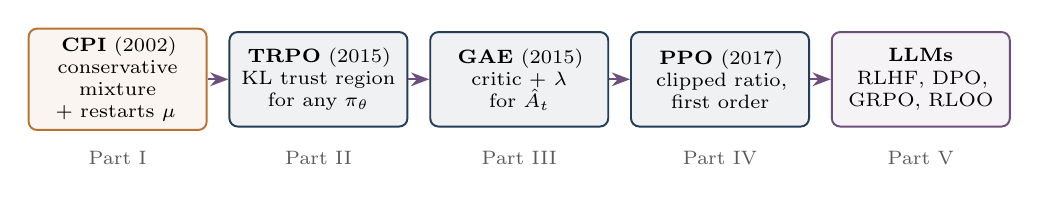
\begin{tikzpicture}[font=\scriptsize, >=Stealth,
    p/.style={rectangle, rounded corners=3pt, line width=0.7pt, text width=2.05cm,
      align=center, minimum height=1.2cm, inner sep=3pt}]
  \node[p, cbox=AtlasWarm] (cpi) at (0,0) {\textbf{CPI} (2002)\\ conservative mixture\\ + restarts $\mu$};
  \node[p, cbox=AtlasCool] (trpo) at (2.55,0) {\textbf{TRPO} (2015)\\ KL trust region\\ for any $\pi_\theta$};
  \node[p, cbox=AtlasCool] (gae) at (5.1,0) {\textbf{GAE} (2015)\\ critic + $\lambda$\\ for $\hat A_t$};
  \node[p, cbox=AtlasCool] (ppo) at (7.65,0) {\textbf{PPO} (2017)\\ clipped ratio,\\ first order};
  \node[p, cbox=AtlasSlate] (llm) at (10.2,0) {\textbf{LLMs}\\ RLHF, DPO,\\ GRPO, RLOO};
  \foreach \a/\b in {cpi/trpo, trpo/gae, gae/ppo, ppo/llm} \draw[->, thick, AtlasSlate] (\a) -- (\b);
  \node[font=\scriptsize, NoteGray] at (2.55,-1.0) {Part II};
  \node[font=\scriptsize, NoteGray] at (0,-1.0) {Part I};
  \node[font=\scriptsize, NoteGray] at (5.1,-1.0) {Part III};
  \node[font=\scriptsize, NoteGray] at (7.65,-1.0) {Part IV};
  \node[font=\scriptsize, NoteGray] at (10.2,-1.0) {Part V};
\end{tikzpicture}
\end{center}

\begin{notebox}
\textbf{Two normalizations.} CPI (Part I) uses \textbf{normalized} values: $V_\pi=(1-\gamma)\E[\sum_t\gamma^t r_t]\in[0,R]$, and $d_{\pi,\mu}$ sums to 1.
TRPO, GAE and PPO use \textbf{unnormalized} returns $\eta=\E[\sum_t\gamma^t r_t]$ and visitations $\rho_\pi$. Constants in the bounds differ by factors of $(1-\gamma)$.
\end{notebox}

\textbf{Sources} (local copies in \texttt{seminar/RL\_algos/papers/})

\begin{center}
\small
\begin{tabularx}{\linewidth}{@{}l L l@{}}
\toprule
\textbf{Key} & \textbf{Paper} & \textbf{Part} \\
\midrule
K\&L 2002 & Kakade \& Langford, \emph{Approximately Optimal Approximate Reinforcement Learning} (ICML) & I \\
TRPO & Schulman et al., \emph{Trust Region Policy Optimization} (ICML 2015) & II \\
GAE & Schulman et al., \emph{High-Dimensional Continuous Control Using Generalized Advantage Estimation} (ICLR 2016) & III \\
PPO & Schulman et al., \emph{Proximal Policy Optimization Algorithms} (arXiv 2017) & IV \\
Human prefs & Christiano et al., \emph{Deep RL from Human Preferences} (NeurIPS 2017) & V \\
InstructGPT & Ouyang et al., \emph{Training Language Models to Follow Instructions with Human Feedback} (NeurIPS 2022) & V \\
DPO & Rafailov et al., \emph{Direct Preference Optimization} (NeurIPS 2023) & V \\
DeepSeekMath & Shao et al., \emph{DeepSeekMath} --- introduces GRPO (arXiv 2024) & V \\
RLOO & Ahmadian et al., \emph{Back to Basics: REINFORCE-Style Optimization \ldots} (ACL 2024) & V \\
\bottomrule
\end{tabularx}
\end{center}


\tableofcontents
\clearpage

% ===========================================================================
%  PART I --- CONSERVATIVE POLICY ITERATION (Kakade & Langford, 2002)
% ===========================================================================
\clearpage
\part{Conservative Policy Iteration}

\partintro{\textbf{The question of Part I:} approximate methods give no guarantee that an update helps.
CPI adds two fixes --- a \textbf{conservative (mixture) step} and a \textbf{restart distribution} $\mu$ --- and gets answers to three questions: what improves, how to verify it, and how good the result is.}

% ---------------------------------------------------------------------------
\section{Setting and notation}
% ---------------------------------------------------------------------------

\paper{Approximately Optimal Approximate Reinforcement Learning}
  {Kakade \& Langford}{ICML 2002}
  {Conservative Policy Iteration (CPI)}
  {approximately\_optimal\_approximate\_RL.md}

\subsection{Assumptions}

A finite MDP $(S, D, A, \mathcal{R}, P)$:

\begin{enumerate}
  \item \textbf{Finite} state and action spaces: $|S|, |A| < \infty$. \hfill {\footnotesize\color{NoteGray}TRPO later allows continuous spaces}
  \item \textbf{Bounded rewards}: $\mathcal{R}: S \times A \to [0, R]$.
  \item \textbf{Discounted}: $\gamma \in [0,1)$.
  \item \textbf{Unknown dynamics}: $P(s';s,a)$ is not given; we can only \textbf{sample} transitions (model-free).
  \item \textbf{Start-state distribution} $D$. The goal is
  \begin{gather*}
    \eta_D(\pi) = \E_{s_0\sim D}\big[V_\pi(s_0)\big].
  \end{gather*}
\end{enumerate}

\begin{notebox}
Finiteness does not help by itself: $P$ is unknown, so $V_\pi$ can only be \emph{estimated} from rollouts, never computed by dynamic programming. The paper also assumes an approximate greedy policy chooser (a black box); it enters with the algorithm (\S\ref{sec:cpi-alg}).
\end{notebox}

\subsection{Why the start distribution $D$ matters}

\begin{center}
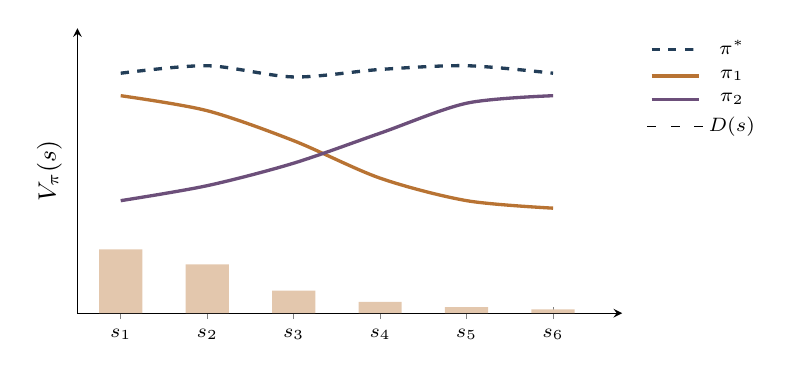
\begin{tikzpicture}
\begin{axis}[notes, width=8.5cm, height=5.2cm, ymin=0, ymax=3.8, xmin=0, xmax=6.3,
    xtick={0.5,1.5,...,5.5}, xticklabels={$s_1$,$s_2$,$s_3$,$s_4$,$s_5$,$s_6$},
    ytick=\empty, ylabel={$V_\pi(s)$}, legend pos=outer north east, legend style={font=\scriptsize}]
  \addplot[AtlasAccent, very thick, dashed, smooth] coordinates {(0.5,3.2)(1.5,3.3)(2.5,3.15)(3.5,3.25)(4.5,3.3)(5.5,3.2)};
  \addlegendentry{$\pi^*$}
  \addplot[AtlasWarm, very thick, smooth] coordinates {(0.5,2.9)(1.5,2.7)(2.5,2.3)(3.5,1.8)(4.5,1.5)(5.5,1.4)};
  \addlegendentry{$\pi_1$}
  \addplot[AtlasSlate, very thick, smooth] coordinates {(0.5,1.5)(1.5,1.7)(2.5,2.0)(3.5,2.4)(4.5,2.8)(5.5,2.9)};
  \addlegendentry{$\pi_2$}
  \addplot[ybar, bar width=0.5, fill=AtlasWarm!40, draw=none, line width=0pt]
    coordinates {(0.5,0.85)(1.5,0.65)(2.5,0.3)(3.5,0.15)(4.5,0.08)(5.5,0.05)};
  \addlegendentry{$D(s)$}
\end{axis}
\end{tikzpicture}
\end{center}

\begin{pair}[3]
\begin{slatebox}[title={Exact}]
\small $\pi^*$ is on top at \textbf{every} state $\Rightarrow$ $D$ is irrelevant.
\end{slatebox}
\begin{warmbox}[title={Approximate}]
\small Curves \textbf{cross}: a restricted class $\{\pi_\theta\}$ and limited data.
\end{warmbox}
\begin{coolbox}[title={Rank by $D$}]
\small $\eta_D(\pi)=\sum_s D(s)V_\pi(s)$. Here $\pi_1$ wins.
\end{coolbox}
\end{pair}

\begin{keybox}
$D$ comes from the \textbf{application} (robot start poses, game openings, user prompts). It is fixed by the problem, like $\mathcal R$ and $P$, and it \textbf{defines the goal}. The restart distribution $\mu$ (later) is different: we choose it, and it only shapes the \emph{learning signal}.
\end{keybox}

Two reasons why the curves cross:
\begin{enumerate}
  \item \textbf{Representation} --- $\pi^*$ may not be in the class. Persists with unlimited data.
  \item \textbf{Estimation} --- even in the tabular case CPI stops with $\OPT(\PA_{\pi,\mu})<2\varepsilon$ (Thm.~4.4); the leftover error is uneven across states (larger where samples are rare). A finite-data effect.
\end{enumerate}

\src{K\&L Sec.~2--3. ``We only consider the case where the goal of the agent is to maximize the $\gamma$ discounted average reward from the starting state distribution $D$.''}

\subsection{Notation: $V$, $Q$, $A$, $d$, $\eta$}

Five quantities, each built on the previous one.

\begin{defbox}{value, action value, advantage (normalized)}
\begin{gather*}
  V_\pi(s) = (1-\gamma)\,\E\Big[\textstyle\sum_{t} \gamma^t \mathcal{R}(s_t,a_t) \,\Big|\, \pi, s_0{=}s\Big] \\
  Q_\pi(s,a) = (1-\gamma)\mathcal{R}(s,a) + \gamma\,\E_{s'}\big[V_\pi(s')\big], \qquad V_\pi(s) = \E_{a\sim\pi(\cdot|s)}\big[Q_\pi(s,a)\big] \\
  A_\pi(s,a) = Q_\pi(s,a) - V_\pi(s)
\end{gather*}
\end{defbox}

\begin{center}
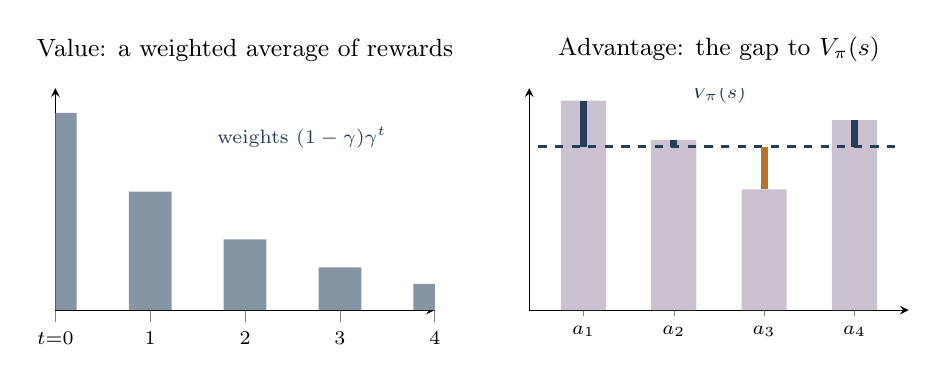
\begin{tikzpicture}
\begin{axis}[notes, name=v, width=6.4cm, height=4.4cm, ybar, bar width=0.45, ymin=0, ymax=1.35,
    xtick={0,...,4}, xticklabels={$t{=}0$,1,2,3,4}, ytick=\empty,
    title={\small Value: a weighted average of rewards}]
  \addplot[fill=AtlasAccent!55, draw=none] coordinates {(0,1.2)(1,0.72)(2,0.43)(3,0.26)(4,0.16)};
  \node[font=\scriptsize, AtlasAccent] at (axis cs:2.6,1.05) {weights $(1-\gamma)\gamma^t$};
\end{axis}
\begin{axis}[notes, at={(v.east)}, anchor=west, xshift=1.2cm, width=6.4cm, height=4.4cm,
    ymin=0, ymax=3.6, xmin=0.4, xmax=4.6, xtick={1,...,4}, xticklabels={$a_1$,$a_2$,$a_3$,$a_4$},
    ytick=\empty, title={\small Advantage: the gap to $V_\pi(s)$}]
  \addplot[ybar, bar width=0.5, fill=AtlasSlate!35, draw=none] coordinates {(1,3.4)(2,2.76)(3,1.96)(4,3.08)};
  \addplot[AtlasAccent, very thick, dashed, domain=0.5:4.5] {2.65};
  \node[font=\scriptsize, AtlasAccent, anchor=south] at (axis cs:2.5,3.2) {$V_\pi(s)$};
  \draw[AtlasCool, line width=2.5pt] (axis cs:1,2.65) -- (axis cs:1,3.4);
  \draw[AtlasCool, line width=2.5pt] (axis cs:2,2.65) -- (axis cs:2,2.76);
  \draw[AtlasCool, line width=2.5pt] (axis cs:4,2.65) -- (axis cs:4,3.08);
  \draw[AtlasWarm, line width=2.5pt] (axis cs:3,2.65) -- (axis cs:3,1.96);
\end{axis}
\end{tikzpicture}
\end{center}

\begin{itemize}
  \item \textbf{Value.} The weights $(1-\gamma)\gamma^t$ sum to 1, so $V_\pi$ is an \emph{average} of rewards: $V\in[0,R]$.
  \item \textbf{Action value.} Take $a$ first, then follow $\pi$. $V_\pi$ is the $\pi$-weighted average of the bars.
  \item \textbf{Advantage.} Gaps to the $V$ line. Weighted by $\pi$ they cancel: $\E_{a\sim\pi}[A_\pi(s,a)]=0$.
        A different $\pi'$ that favors the {\color{AtlasCool}\textbf{positive}} gaps gets $\E_{a\sim\pi'}[A_\pi(s,a)]>0$ --- the seed of the \emph{policy advantage} (\S\ref{sec:pa}).
\end{itemize}

\begin{defbox}{discounted visitation and objective}
\begin{gather*}
  d_{\pi,D}(s) = (1-\gamma)\textstyle\sum_{t} \gamma^t \Pr(s_t = s;\, \pi, D), \qquad
  \eta_D(\pi) = \E_{s\sim D}\big[V_\pi(s)\big] = \E_{s\sim d_{\pi,D},\,a\sim\pi}\big[\mathcal R(s,a)\big]
\end{gather*}
\end{defbox}

\begin{pair}
\begin{coolbox}[title={$d_{\pi,D}$: the whole trajectory}]
\small Where $\pi$ spends its time when started from $s_0\sim D$; early steps weigh more.
\end{coolbox}
\begin{warmbox}[title={$D$: only $s_0$}]
\small The distribution of the first state. Easy to confuse with $d_{\pi,D}$.
\end{warmbox}
\end{pair}

\begin{notebox}
\begin{itemize}[leftmargin=*]
  \item Unnormalized visitation: $\rho_\pi=(I-\gamma P_\pi^\top)^{-1}D$ --- linear in $D$, nonlinear in $\pi$.
  \item Training is on-policy: $\pi$ shapes the visitation used for the next update --- a \textbf{feedback loop}, not a fixed reweighting.
  \item TRPO drops the $(1-\gamma)$ factor; this changes the constants in its bounds.
\end{itemize}
\end{notebox}

% ---------------------------------------------------------------------------
\section{Three questions for any approximate method}
% ---------------------------------------------------------------------------

\begin{tcolorbox}[notes, colback=GoodGreen!5, colframe=GoodGreen, colbacktitle=GoodGreen, title={The three questions (K\&L Sec.~3)}]
\begin{enumerate}[label=\textbf{Q\arabic*}]
  \item Is there a \textbf{performance measure} that is guaranteed to \textbf{improve at every step}?
  \item How hard is it to \textbf{verify} that a given update improves this measure?
  \item What \textbf{performance level} is reached after a \textbf{reasonable number} of updates?
\end{enumerate}
\end{tcolorbox}

{\small Not ``what is the asymptotic policy?'' --- only policies reachable in reasonable time.}

\begin{center}
\small
\begin{tabular}{l c c c}
\toprule
 & \textbf{Q1} improve & \textbf{Q2} verify & \textbf{Q3} performance \\
\midrule
{\color{AtlasWarm}\textbf{Approximate value functions}} & weak & weak & weak \\
{\color{AtlasCool}\textbf{Policy gradients}} & \textbf{good} & poor & poor \\
{\color{GoodGreen}\textbf{CPI}} & \cmark & \cmark & \cmark{} (up to a mismatch factor) \\
\bottomrule
\end{tabular}
\end{center}

The next two sections show why the first two rows look like this (\textbf{Gap 1} and \textbf{Gap 2}).

% ---------------------------------------------------------------------------
\section{Gap 1: approximate value functions}
% ---------------------------------------------------------------------------

\subsection{Reminder: approximate policy iteration}

\begin{center}
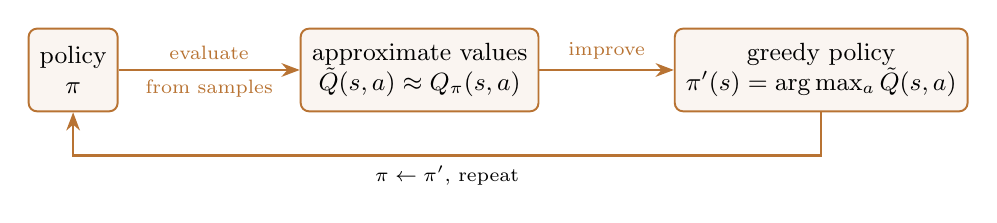
\begin{tikzpicture}[>=Stealth, b/.style={fl, cbox=AtlasWarm, minimum height=1.05cm}]
  \node[b] (pi) at (0,0) {policy\\ $\pi$};
  \node[b] (q) at (4.4,0) {approximate values\\ $\tilde Q(s,a)\approx Q_\pi(s,a)$};
  \node[b] (g) at (9.5,0) {greedy policy\\ $\pi'(s)=\arg\max_a \tilde Q(s,a)$};
  \draw[->, thick, AtlasWarm] (pi) -- node[above, font=\scriptsize]{evaluate} node[below, font=\scriptsize]{from samples} (q);
  \draw[->, thick, AtlasWarm] (q) -- node[above, font=\scriptsize]{improve} (g);
  \draw[->, thick, AtlasWarm] (g.south) -- ++(0,-0.55) -| (pi.south) node[pos=0.25, below, font=\scriptsize, text=black]{$\pi\leftarrow\pi'$, repeat};
\end{tikzpicture}
\end{center}

Exact policy iteration, with $Q_\pi$ replaced by an \textbf{estimate} $\tilde Q$.

\begin{warmbox}[title={Example: Q-learning with a function approximator $\tilde Q_w$}]
\begin{gather*}
  w \leftarrow w + \alpha\,\big(y_t - \tilde Q_w(s_t,a_t)\big)\,\nabla_w \tilde Q_w(s_t,a_t), \qquad
  y_t = (1-\gamma)\,r_t + \gamma \max_{a'} \tilde Q_w(s_{t+1},a')
\end{gather*}
\begin{itemize}
  \item The $\max$ is the greedy step: evaluate and improve happen \textbf{together}.
  \item Strictly, this is approximate \emph{value} iteration; with a neural network it is DQN.
  \item The target $y_t$ is one choice of many (next subsection).
\end{itemize}
\end{warmbox}

\subsection{How is $\tilde Q$ estimated? From TD(0) to Monte Carlo}

\begin{center}
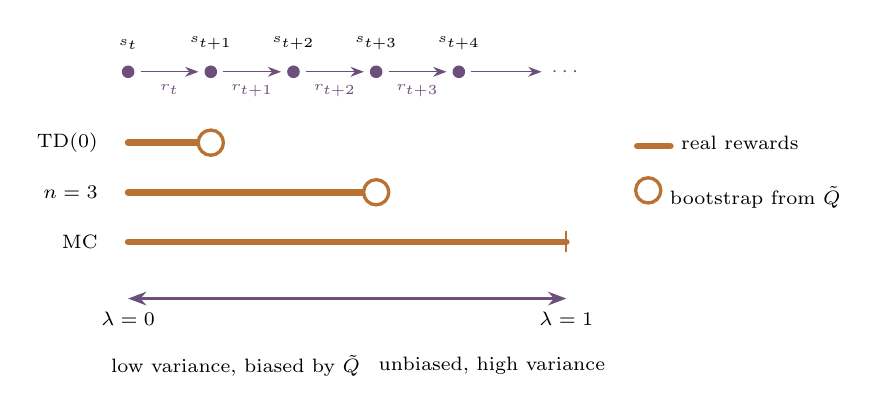
\begin{tikzpicture}[x=1.05cm, y=0.9cm, >=Stealth,
    st/.style={circle, fill=AtlasSlate, minimum size=0.16cm, inner sep=0pt},
    real/.style={AtlasWarm, line width=2.4pt, line cap=round},
    boot/.style={circle, draw=AtlasWarm, very thick, fill=white, minimum size=0.32cm, inner sep=0pt},
    lab/.style={font=\scriptsize, anchor=east}]
  \foreach \i/\n in {0/t, 1/t{+}1, 2/t{+}2, 3/t{+}3, 4/t{+}4} {
    \node[st] (s\i) at (\i,0) {};
    \node[font=\tiny, above=2pt of s\i] {$s_{\n}$};}
  \foreach \i/\j/\r in {0/1/t, 1/2/t{+}1, 2/3/t{+}2, 3/4/t{+}3}
    \draw[->, AtlasSlate, shorten <=2pt, shorten >=2pt] (s\i) -- node[below=1pt, font=\tiny]{$r_{\r}$} (s\j);
  \draw[->, AtlasSlate, shorten <=2pt] (s4) -- (5.0,0) node[right, font=\scriptsize]{$\cdots$};
  \node[lab] at (-0.25,-1.0) {TD(0)};
  \draw[real] (0,-1.0) -- (1,-1.0); \node[boot] at (1,-1.0) {};
  \node[lab] at (-0.25,-1.7) {$n=3$};
  \draw[real] (0,-1.7) -- (3,-1.7); \node[boot] at (3,-1.7) {};
  \node[lab] at (-0.25,-2.4) {MC};
  \draw[real] (0,-2.4) -- (5.3,-2.4); \draw[AtlasWarm, thick] (5.3,-2.55) -- (5.3,-2.25);
  \node[font=\scriptsize, anchor=west] at (6.0,-1.0) {\tikz\draw[real] (0,0) -- (0.4,0); real rewards};
  \node[font=\scriptsize, anchor=west] at (6.0,-1.7) {\tikz\node[boot] {}; bootstrap from $\tilde Q$};
  \draw[<->, thick, AtlasSlate] (0,-3.2) -- (5.3,-3.2);
  \node[font=\scriptsize, below] at (0,-3.25) {$\lambda=0$};
  \node[font=\scriptsize, below] at (5.3,-3.25) {$\lambda=1$};
  \node[font=\scriptsize, align=center] at (1.3,-4.15) {low variance, biased by $\tilde Q$};
  \node[font=\scriptsize, align=center] at (4.4,-4.15) {unbiased, high variance};
\end{tikzpicture}
\end{center}

\begin{center}
\small
\begin{tabular}{l l l}
\toprule
\textbf{Target} & \textbf{Formula} & \textbf{Trade-off} \\
\midrule
TD(0) & $y_t^{(1)} = (1-\gamma)\,r_t + \gamma\,\tilde Q(s_{t+1},a_{t+1})$ & one reward, then trust $\tilde Q$ \\
$n$-step & $y_t^{(n)} = (1-\gamma)\sum_{k=0}^{n-1}\gamma^k r_{t+k} + \gamma^n\,\tilde Q(s_{t+n},a_{t+n})$ & in between \\
Monte Carlo & $y_t^{(\infty)} = (1-\gamma)\sum_{k\ge0}\gamma^k r_{t+k}$ & only real rewards; wait for the end \\
TD($\lambda$) & $y_t^{\lambda} = (1-\lambda)\sum_{n\ge1}\lambda^{n-1}\,y_t^{(n)}$ & average over all $n$ \\
\bottomrule
\end{tabular}
\end{center}

\begin{notebox}
The weights $(1-\lambda)\lambda^{n-1}$ sum to 1: $\lambda=0$ gives TD(0), $\lambda\to1$ gives Monte Carlo. The \textbf{same $\lambda$ trade-off returns for advantages} in GAE (Part III). Background from Sutton \& Barto, Ch.~6, 7, 12; not in K\&L.
\end{notebox}

\subsection{The bound: no improvement guarantee}

Measure the approximation error \textbf{everywhere} ($\ell_\infty$):
\begin{gather*}
  \varepsilon = \max_s \big|\tilde V(s) - V_\pi(s)\big|.
\end{gather*}

\begin{thmbox}{Approximate greedy step (Bertsekas \& Tsitsiklis; K\&L Eq.~3.1)}
If $\pi'$ is greedy with respect to $\tilde V$, then
\begin{gather*}
  V_{\pi'}(s) \;\ge\; V_\pi(s) - \frac{2\gamma\varepsilon}{1-\gamma} \qquad \forall s.
\end{gather*}
\end{thmbox}

\begin{minipage}[c]{0.5\linewidth}
\centering
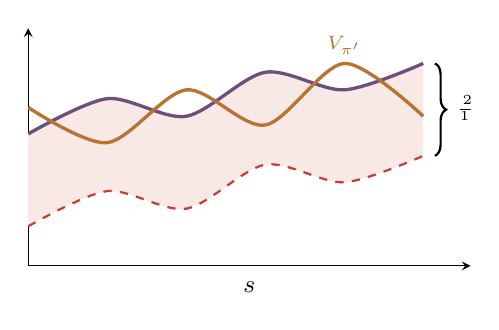
\begin{tikzpicture}
\begin{axis}[notes, width=7.2cm, height=4.6cm, xmin=0, xmax=5.6, ymin=0.5, ymax=3.2,
    xtick=\empty, ytick=\empty, xlabel={$s$}]
  \addplot[name path=top, AtlasSlate, very thick, smooth] coordinates {(0,2.0)(1,2.4)(2,2.2)(3,2.7)(4,2.5)(5,2.8)};
  \addplot[name path=bot, BadRed, thick, dashed, smooth] coordinates {(0,0.95)(1,1.35)(2,1.15)(3,1.65)(4,1.45)(5,1.75)};
  \addplot[BadRed!12] fill between[of=top and bot];
  \addplot[AtlasWarm, very thick, smooth] coordinates {(0,2.3)(1,1.9)(2,2.5)(3,2.1)(4,2.8)(5,2.2)};
  \node[font=\scriptsize, AtlasSlate, anchor=east] at (axis cs:0,2.0) {$V_\pi$};
  \node[font=\scriptsize, AtlasWarm] at (axis cs:4.0,3.0) {$V_{\pi'}$};
  \draw[decorate, decoration={brace, amplitude=4pt, mirror}, thick] (axis cs:5.15,1.75) -- (axis cs:5.15,2.8)
    node[midway, right=4pt, font=\scriptsize]{$\frac{2\gamma\varepsilon}{1-\gamma}$};
\end{axis}
\end{tikzpicture}
\end{minipage}\hfill
\begin{minipage}[c]{0.46\linewidth}
\begin{itemize}
  \item $V_{\pi'}$ may sit anywhere above the dashed line --- \textbf{also below} $V_\pi$.
  \item Only ``won't get \textbf{much worse}''; never ``gets better''.
  \item The $\ell_\infty$ requirement is strong: one badly estimated state is enough to make the bound loose.
\end{itemize}
\end{minipage}

\begin{warnbox}
Weak answers to all three questions: no measure is guaranteed to improve (Q1), so verifying an update (Q2) has nothing to check against, and nothing bounds the performance after a number of updates (Q3).
\end{warnbox}

\subsection{The bound is tight: a two-state example}

\begin{minipage}[c]{0.44\linewidth}
\centering
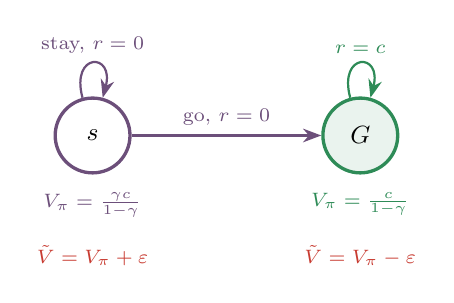
\begin{tikzpicture}[>=Stealth, st/.style={circle, draw=AtlasSlate, very thick, minimum size=0.95cm, font=\small}]
  \node[st] (s) at (0,0) {$s$};
  \node[st, draw=GoodGreen, fill=GoodGreen!10] (g) at (3.4,0) {$G$};
  \draw[->, thick, AtlasSlate] (s) -- node[above, font=\scriptsize]{go, $r=0$} (g);
  \draw[->, thick, AtlasSlate] (s) edge[loop above, looseness=6] node[above, font=\scriptsize]{stay, $r=0$} (s);
  \draw[->, thick, GoodGreen] (g) edge[loop above, looseness=6] node[above, font=\scriptsize]{$r=c$} (g);
  \node[font=\scriptsize, AtlasSlate, below=3pt of s] {$V_\pi = \tfrac{\gamma c}{1-\gamma}$};
  \node[font=\scriptsize, GoodGreen, below=3pt of g] {$V_\pi = \tfrac{c}{1-\gamma}$};
  \node[font=\scriptsize, BadRed, below=22pt of s] {$\tilde V = V_\pi + \varepsilon$};
  \node[font=\scriptsize, BadRed, below=22pt of g] {$\tilde V = V_\pi - \varepsilon$};
\end{tikzpicture}\\[2pt]
{\scriptsize $\pi$ = go. Set $c=2\varepsilon$. Unnormalized values.}
\end{minipage}\hfill
\begin{minipage}[c]{0.53\linewidth}
\begin{enumerate}
  \item $\pi$ goes to $G$ and collects $c$ forever.
  \item $\tilde V$ is off by $\varepsilon$: too \textbf{high} at $s$, too \textbf{low} at $G$.
  \item Greedy w.r.t.\ $\tilde V$ at $s$ compares
  \begin{gather*}
    \underbrace{\gamma\big(V_\pi(s)+\varepsilon\big)}_{\text{stay}} \;=\; \underbrace{\gamma\big(V_\pi(G)-\varepsilon\big)}_{\text{go}}
  \end{gather*}
  a tie, since $V_\pi(G)-V_\pi(s)=c=2\varepsilon$. So $\pi'$ may stay forever: $V_{\pi'}(s)=0$.
\end{enumerate}
\end{minipage}

\begin{warnbox}[title={The loss equals the bound}]
At $s$: $V_\pi(s)-V_{\pi'}(s) = \frac{\gamma c}{1-\gamma} = \frac{2\gamma\varepsilon}{1-\gamma}$. \quad At $G$: one action only, so the loss is $0$.\\
Two errors of size $\varepsilon$, in opposite directions, make the greedy policy stop moving; the $\frac{1}{1-\gamma}$ sums the lost reward over the horizon.
\end{warnbox}

\begin{notebox}
Our own minimal example. With $c$ slightly below $2\varepsilon$ staying is strictly preferred and the loss gets arbitrarily close to the bound. B\&T (\emph{Neuro-Dynamic Programming}, Ex.~6.4) show tightness of the related API bound $\limsup_k\|V_{\pi_k}-V^*\|_\infty\le\frac{2\gamma\varepsilon}{(1-\gamma)^2}$; the one-step form is due to Singh \& Yee (1994).
\end{notebox}

% ---------------------------------------------------------------------------
\section{Gap 2: policy gradients}
% ---------------------------------------------------------------------------

\subsection{Reminder: policy gradient methods}

\begin{center}
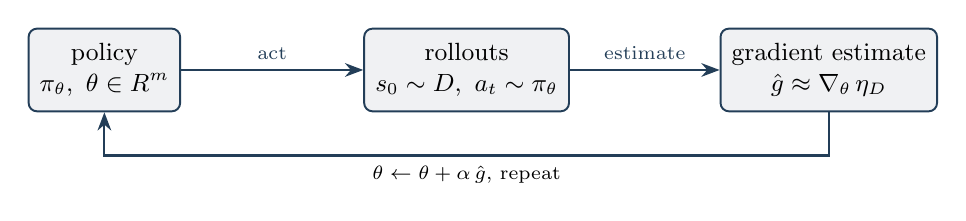
\begin{tikzpicture}[>=Stealth, b/.style={fl, cbox=AtlasCool, minimum height=1.05cm}]
  \node[b] (pi) at (0,0) {policy\\ $\pi_\theta,\ \theta\in\mathbb{R}^m$};
  \node[b] (r) at (4.6,0) {rollouts\\ $s_0\sim D,\ a_t\sim\pi_\theta$};
  \node[b] (g) at (9.2,0) {gradient estimate\\ $\hat g\approx\nabla_\theta\,\eta_D$};
  \draw[->, thick, AtlasCool] (pi) -- node[above, font=\scriptsize]{act} (r);
  \draw[->, thick, AtlasCool] (r) -- node[above, font=\scriptsize]{estimate} (g);
  \draw[->, thick, AtlasCool] (g.south) -- ++(0,-0.55) -| (pi.south) node[pos=0.25, below, font=\scriptsize, text=black]{$\theta\leftarrow\theta+\alpha\,\hat g$, repeat};
\end{tikzpicture}
\end{center}

\begin{thmbox}{Policy gradient theorem (Sutton et al.; normalized)}
\begin{gather*}
  \nabla_\theta\, \eta_D = \frac{1}{1-\gamma}\sum_{s,a} d_{\pi,D}(s)\, \nabla_\theta \pi(a;s)\, Q_\pi(s,a)
\end{gather*}
\end{thmbox}

Small steps uphill on $\eta_D$ \emph{itself} $\Rightarrow$ a \textbf{good answer to Q1}.

\begin{coolbox}[title={Example: REINFORCE with a Gibbs (softmax) policy}]
\begin{gather*}
  \pi_\theta(a;s) = \frac{e^{\theta_{sa}}}{\sum_b e^{\theta_{sb}}}, \qquad
  \hat g \;\propto\; \sum_t \nabla_\theta \log \pi_\theta(a_t;s_t)\, \hat Q_t
\end{gather*}
$\hat Q_t$: the return observed after step $t$. The Gibbs class is the one of Example~2 below. Details: App.~\ref{app:gibbs}.
\end{coolbox}

\subsection{Policy gradient is stochastic gradient ascent}

\begin{center}
\small
\begin{tabular}{r l l}
\toprule
 & {\color{AtlasSlate}\textbf{Stochastic gradient descent}} & {\color{AtlasCool}\textbf{Policy gradient}} \\
\midrule
{\color{NoteGray}objective} & $\min_w J(w)=\E_X[f(w,X)]$ & $\max_\theta \eta_D(\theta)=\E_{\tau\sim\pi_\theta}[R(\tau)]$ \\
{\color{NoteGray}looking for} & $\nabla J(w)=0$ & $\nabla_\theta\eta_D(\theta)=0$ \\
{\color{NoteGray}one sample} & $x_k\sim X$ & rollout $\tau_k$: $s_0\sim D$, $a_t\sim\pi_{\theta_k}$ \\
{\color{NoteGray}update} & $w_{k+1}=w_k-a_k\nabla_w f(w_k,x_k)$ & $\theta_{k+1}=\theta_k+a_k\hat g_k$ \\
{\color{NoteGray}noise} & $\eta_k=\nabla_w f(w_k,x_k)-\nabla J(w_k)$ & $\eta_k=\hat g_k-\nabla_\theta\eta_D(\theta_k)$ \\
\bottomrule
\end{tabular}
\end{center}

\begin{notebox}
\textbf{The twist.} In SGD the distribution of $X$ does not depend on $w$. Here the trajectories come from $\pi_\theta$ itself, so $\nabla\eta_D\neq\E[\nabla R]$. The log-derivative trick (REINFORCE) still gives an \textbf{unbiased} $\hat g_k$ --- App.~\ref{app:logderiv}. Notation clash: $\eta_k$ (noise) is not $\eta_D$ (performance).
\end{notebox}

\subsection{What SGD theory guarantees}

\textbf{Convergence conditions} (Robbins \& Monro, 1951) --- each has a role:

\begin{center}
\small
\begin{tabularx}{\linewidth}{@{}l l L@{}}
\toprule
\textbf{Condition} & \textbf{Formula} & \textbf{Role} \\
\midrule
1.~Curvature & $0<c_1\le\nabla_w^2 f(w,X)\le c_2$ & one minimizer; bounds on the rate \\
2.~Unbiased noise & $\E[\eta_k\mid\mathcal H_k]=0$ & steps point the right way on average \\
3.~Finite variance & $\E[\eta_k^2\mid\mathcal H_k]<\infty$ & with 4, the summed noise stays finite \\
4.~Step sizes & $\sum_k a_k=\infty$, \ $\sum_k a_k^2<\infty$ & reach any distance; e.g.\ $a_k=c/k$ \\
\bottomrule
\end{tabularx}
\end{center}
{\footnotesize\color{NoteGray}$\mathcal H_k$: the history so far, $w_0,x_0,\dots,x_{k-1}$. Under 1--4: $w_k\to w^*$ almost surely.}

\textbf{Sample complexity} --- samples needed to be $\epsilon$-close with probability $\ge1-\delta$:
\begin{gather*}
  N(\epsilon,\delta) = \min\Big\{ N \in \mathbb{N} \;\Big|\; \mathbb{P}\big(\|w_k - w^*\| \le \epsilon\big) \ge 1-\delta \ \text{ for all } k \ge N \Big\}
\end{gather*}

\begin{center}
\small
\begin{tabularx}{\linewidth}{@{}l L@{}}
\toprule
\textbf{Setting} & \textbf{Guarantee} \\
\midrule
Convex, smooth & global optimum: $N(\epsilon,\delta)=O\big(\sigma^2/(c_1^2\epsilon^2\delta)\big)$ \hfill {\scriptsize\color{NoteGray}Nemirovski et al.\ 2009 + Markov} \\
Non-convex, smooth & stationary point only: $\E\|\nabla J(w_R)\|\le\epsilon$ after $K=O(\sigma^2/\epsilon^4)$, $w_R$ a random iterate \hfill {\scriptsize\color{NoteGray}Ghadimi \& Lan 2013} \\
{\color{AtlasCool}Non-convex, non-smooth} & {\color{AtlasCool}weaker still: near-stationary points, special classes --- \textbf{policy gradients with neural nets live here}} \\
\bottomrule
\end{tabularx}
\end{center}

\begin{keybox}[title={What carries over}]
The convex case shows \textbf{what drives} $N$: the noise $\sigma^2$ and the curvature $c_1$. More noise means more samples; flat regions are slow.
\end{keybox}

\subsection{The signal-to-noise reality}

\begin{enumerate}
  \item Finite variance is enough for convergence \emph{in the limit}.
  \item In practice $N$ depends on the \textbf{signal-to-noise ratio}. Averaging $n$ samples leaves noise $\sigma/\sqrt n$; just to get the \emph{direction} right:
  \begin{gather*}
    n \gtrsim \sigma^2/\|\nabla J\|^2.
  \end{gather*}
  \item \textbf{Link to curvature.} Strong convexity gives $\|\nabla J(w)\|\ge c_1\|w-w^*\|$, so at distance $\epsilon$:
  \begin{gather*}
    n \gtrsim \sigma^2/(c_1\epsilon)^2 \qquad \text{(the convex-row $N$, without the $1/\delta$)}.
  \end{gather*}
  \item \textbf{Flat} ($c_1$ small) or $\|\nabla J\|\to0$: the noise dominates and $n$ becomes intractable.
\end{enumerate}

\begin{notebox}
The theory's $1/c_1^2$ \emph{is} the signal-to-noise cost. The next two MDPs have an (almost) zero gradient: this picture, in RL.
\end{notebox}

\subsection{Example 1: exploration}
\label{sec:gap2-ex1}

\begin{center}
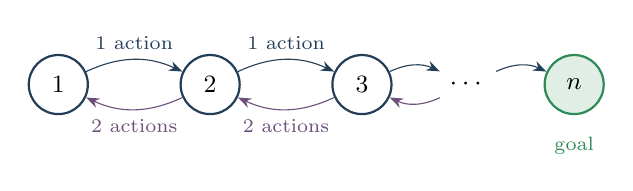
\begin{tikzpicture}[st/.style={circle, draw=AtlasCool, thick, minimum size=0.75cm, font=\small},
                    >=Stealth, node distance=1.15cm]
  \node[st] (s1) {$1$};
  \node[st, right=of s1] (s2) {$2$};
  \node[st, right=of s2] (s3) {$3$};
  \node[right=0.6cm of s3] (dots) {$\cdots$};
  \node[st, right=0.6cm of dots, fill=GoodGreen!15, draw=GoodGreen] (sn) {$n$};
  \foreach \a/\b in {s1/s2, s2/s3} {
    \draw[->, AtlasCool] (\a) to[bend left=25] node[above, font=\scriptsize]{1 action} (\b);
    \draw[->, AtlasSlate] (\b) to[bend left=25] node[below, font=\scriptsize]{2 actions} (\a);}
  \draw[->, AtlasCool] (s3) to[bend left=25] (dots);
  \draw[->, AtlasSlate] (dots) to[bend left=25] (s3);
  \draw[->, AtlasCool] (dots) to[bend left=25] (sn);
  \node[below=0.15cm of sn, font=\scriptsize, GoodGreen] {goal};
\end{tikzpicture}
\end{center}

\begin{itemize}
  \item Two actions move left, one moves right. Uniform random policy: expected time to the goal $= 3(2^n-n-1)\approx10^{15}$ for $n=50$.
  \item Before reaching the goal every sensible gradient estimate is $\mathbf 0$: the right \emph{magnitude}, but \textbf{no direction}.
  \item Importance sampling does not help: the weights would be exponentially large.
\end{itemize}

\subsection{Example 2: plateaus}

\begin{minipage}[c]{0.36\linewidth}
\centering
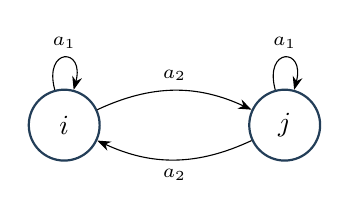
\begin{tikzpicture}[st/.style={circle, draw=AtlasCool, thick, minimum size=0.9cm}, >=Stealth]
  \node[st] (i) at (0,0) {$i$};
  \node[st] (j) at (2.8,0) {$j$};
  \draw[->] (i) to[bend left=25] node[above, font=\scriptsize]{$a_2$} (j);
  \draw[->] (j) to[bend left=25] node[below, font=\scriptsize]{$a_2$} (i);
  \draw[->] (i) to[loop above, looseness=6] node[above, font=\scriptsize]{$a_1$} (i);
  \draw[->] (j) to[loop above, looseness=6] node[above, font=\scriptsize]{$a_1$} (j);
\end{tikzpicture}\\
{\scriptsize Gibbs policy: $\pi(a;s)\propto\exp(\theta_{sa})$}
\end{minipage}\hfill
\begin{minipage}[c]{0.6\linewidth}
\begin{enumerate}
  \item Start: $\rho(i)=0.8$, $\rho(j)=0.2$ \ ($\pi(a_1;i)=0.8$, $\pi(a_1;j)=0.9$).
  \item Raising the self-loop at $i$ \textbf{starves} state $j$.
  \item $\rho(j)$ drops to $\approx10^{-7}$ $\Rightarrow$ nothing is learned at $j$.
  \item Result: an extremely \textbf{flat plateau} (on a $10^7$ time scale).
\end{enumerate}
\end{minipage}

\begin{warnbox}[title={Root cause}]
$\eta_D$ weighs improvements by $d_{\pi,D}$: it is \textbf{insensitive to improvement at unlikely states} --- unlikely under the \emph{current} policy --- even when those states are needed for near-optimal performance.
\end{warnbox}
\src{K\&L Sec.~3.2, Figs.~3.1--3.3.}

\subsection{Gap 2 as covariate shift}

\begin{center}
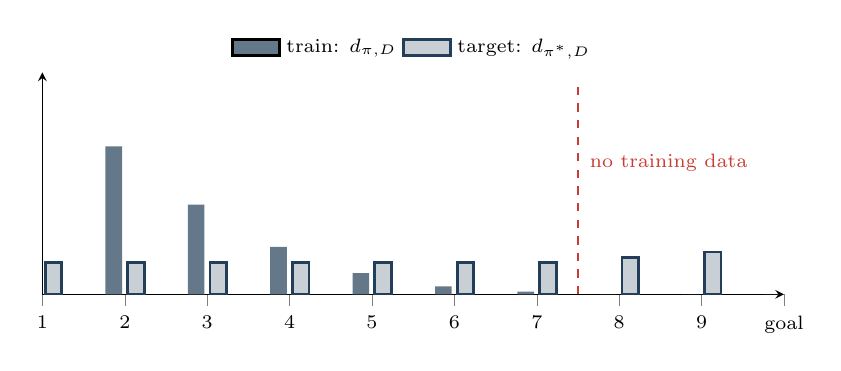
\begin{tikzpicture}
\begin{axis}[notes, width=11cm, height=4.4cm, ybar, bar width=6pt, ymin=0, ymax=0.42,
    xtick={1,...,10}, xticklabels={1,2,3,4,5,6,7,8,9,goal}, ytick=\empty,
    legend style={at={(0.5,1.02)}, anchor=south, legend columns=2}, area legend]
  \addplot[fill=AtlasCool!70, draw=none] coordinates {(1,0.4)(2,0.28)(3,0.17)(4,0.09)(5,0.04)(6,0.015)(7,0.005)(8,0)(9,0)(10,0)};
  \addlegendentry{train: $d_{\pi,D}$}
  \addplot[fill=AtlasAccent!25, draw=AtlasAccent] coordinates {(1,0.06)(2,0.06)(3,0.06)(4,0.06)(5,0.06)(6,0.06)(7,0.06)(8,0.07)(9,0.08)(10,0.37)};
  \addlegendentry{target: $d_{\pi^*,D}$}
  \draw[BadRed, thick, dashed] (axis cs:7.5,0) -- (axis cs:7.5,0.4);
  \node[font=\scriptsize, BadRed] at (axis cs:8.6,0.25) {no training data};
\end{axis}
\end{tikzpicture}
\end{center}

\begin{pair}[3]
\begin{coolbox}[title={Train}]
\small Samples come from where the \textbf{current} $\pi$ goes.
\end{coolbox}
\begin{slatebox}[title={Target}]
\small Near-optimal play needs good actions where $\pi^*$ goes.
\end{slatebox}
\begin{warnbox}[title={No overlap}]
\small Zero gradient (Ex.~1), starved state $j$ (Ex.~2).
\end{warnbox}
\end{pair}

\textbf{Unlike standard covariate shift:}
\begin{enumerate}
  \item the target $d_{\pi^*,D}$ needs $\pi^*$ --- \textbf{unknown};
  \item the data come from $\pi$ itself --- the gap can \textbf{grow} as $\pi$ learns (Ex.~2);
  \item the ``labels'' $A_\pi$ change with every update;
  \item the off-policy fix is a \textbf{product} of per-step ratios $\prod_t\pi/q$ --- exponential in the horizon, not a single ratio $p_{\text{test}}/p_{\text{train}}$.
\end{enumerate}

\begin{keybox}[title={Instead}]
Change \emph{where the data come from}: train from a restart distribution $\mu$, still judged by $\eta_D$. The precise version (a density ratio) is Thm.~6.2.
\end{keybox}

\begin{notebox}
Related: imitation learning (DAgger) --- the learner's own mistakes change which states it visits. Augmentation view: $\mu$-restarts show the learner states it would not reach; unlike classic augmentation, the states are real and the ``labels'' $\hat Q_\pi$ come from real rollouts. The price is reset access.
\end{notebox}

% ---------------------------------------------------------------------------
\section{The two fixes}
% ---------------------------------------------------------------------------

\begin{pair}
\begin{warmbox}[title={1. Conservative update $\to$ Gap 1}]
Don't jump to the greedy policy --- \textbf{mix}:
\begin{gather*}
  \pinew(a;s) = (1-\alpha)\,\pi(a;s) + \alpha\,\pi'(a;s)
\end{gather*}
\begin{itemize}
  \item $\alpha\in[0,1]$ acts as a \textbf{step size}.
  \item $\alpha=1$ is greedy policy iteration.
\end{itemize}
\end{warmbox}
\begin{coolbox}[title={2. Restart distribution $\mu$ $\to$ Gap 2}]
Optimize a measure that weighs states more uniformly:
\begin{gather*}
  \eta_\mu(\pi) = \E_{s\sim\mu}\big[V_\pi(s)\big]
\end{gather*}
\begin{itemize}
  \item $\mu$ is ``exploratory''; the agent can restart from $s\sim\mu$.
  \item $D$: deployment (given). $\mu$: training resets (chosen).
\end{itemize}
\end{coolbox}
\end{pair}

\begin{itemize}
  \item Any \textbf{optimal} policy maximizes both $\eta_\mu$ and $\eta_D$ --- but within a restricted class they can differ.
  \item Sec.~7.2 of the paper: train under $\tilde\mu=(1-\beta)\mu+\beta D$ to keep some weight on $D$.
\end{itemize}

\textbf{How strong is a $\mu$-restart?} Access to the environment, from strongest to weakest:

\begin{center}
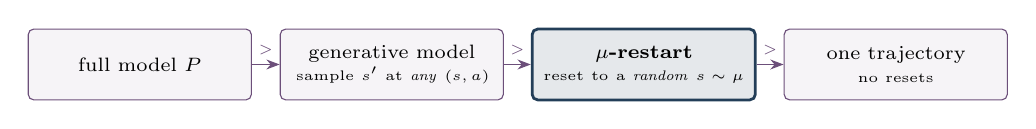
\begin{tikzpicture}[font=\scriptsize, >=Stealth,
    a/.style={rectangle, rounded corners=2pt, draw=AtlasSlate, fill=AtlasSlate!6, text width=2.6cm, align=center, minimum height=0.9cm}]
  \node[a] (p) at (0,0) {full model $P$};
  \node[a] (g) at (3.2,0) {generative model\\ {\tiny sample $s'$ at \emph{any} $(s,a)$}};
  \node[a, draw=AtlasCool, fill=AtlasCool!12, line width=1pt] (m) at (6.4,0) {\textbf{$\mu$-restart}\\ {\tiny reset to a \emph{random} $s\sim\mu$}};
  \node[a] (o) at (9.6,0) {one trajectory\\ {\tiny no resets}};
  \foreach \x/\y in {p/g, g/m, m/o} \draw[->, AtlasSlate] (\x) -- node[above, font=\tiny]{$>$} (\y);
\end{tikzpicture}
\end{center}
{\footnotesize\color{NoteGray}Generative model: Kearns, Mansour \& Ng (1999). $\mu$-restarts need training-time reset access, e.g.\ a simulator, or a lab where the start state can be set.}

\subsection{Roadmap: from the two fixes to the three answers}

\begin{center}
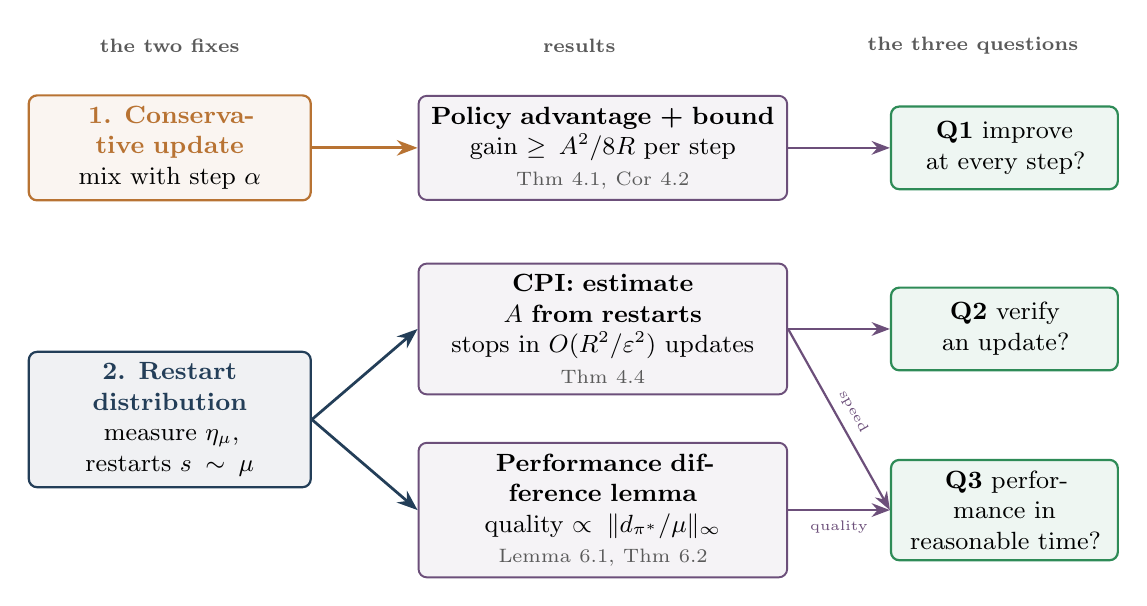
\begin{tikzpicture}[font=\footnotesize, >=Stealth,
    fix/.style={fl, line width=0.8pt, text width=3.3cm, minimum height=1.1cm},
    res/.style={fl, cbox=AtlasSlate, text width=4.4cm, minimum height=1.05cm},
    q/.style={fl, draw=GoodGreen, fill=GoodGreen!8, line width=0.8pt, text width=2.6cm, minimum height=1.05cm}]
  \node[font=\scriptsize\bfseries, NoteGray] at (0,3.6) {the two fixes};
  \node[font=\scriptsize\bfseries, NoteGray] at (5.2,3.6) {results};
  \node[font=\scriptsize\bfseries, NoteGray] at (10.2,3.6) {the three questions};
  \node[fix, cbox=AtlasWarm] (cons) at (0,2.3) {\textbf{\color{AtlasWarm}1. Conservative update}\\ mix with step $\alpha$};
  \node[fix, cbox=AtlasCool] (mu) at (0,-1.15) {\textbf{\color{AtlasCool}2. Restart distribution}\\ measure $\eta_\mu$, restarts $s\sim\mu$};
  \node[res] (a) at (5.5,2.3) {\textbf{Policy advantage + bound}\\ gain $\ge\PA^2/8R$ per step\\ {\scriptsize\color{NoteGray}Thm 4.1, Cor 4.2}};
  \node[res] (b) at (5.5,0) {\textbf{CPI: estimate $\PA$ from restarts}\\ stops in $O(R^2/\varepsilon^2)$ updates\\ {\scriptsize\color{NoteGray}Thm 4.4}};
  \node[res] (c) at (5.5,-2.3) {\textbf{Performance difference lemma}\\ quality $\propto\|d_{\pi^*}/\mu\|_\infty$\\ {\scriptsize\color{NoteGray}Lemma 6.1, Thm 6.2}};
  \node[q] (q1) at (10.6,2.3) {\textbf{Q1} improve at every step?};
  \node[q] (q2) at (10.6,0) {\textbf{Q2} verify an update?};
  \node[q] (q3) at (10.6,-2.3) {\textbf{Q3} performance in reasonable time?};
  \draw[->, line width=1pt, AtlasWarm] (cons) -- (a);
  \draw[->, line width=1pt, AtlasCool] (mu.east) -- (b.west);
  \draw[->, line width=1pt, AtlasCool] (mu.east) -- (c.west);
  \draw[->, AtlasSlate, thick] (a) -- (q1);
  \draw[->, AtlasSlate, thick] (b) -- (q2);
  \draw[->, AtlasSlate, thick] (b.east) -- node[above, sloped, font=\tiny]{speed} (q3.west);
  \draw[->, AtlasSlate, thick] (c) -- node[below, font=\tiny]{quality} (q3);
\end{tikzpicture}
\end{center}

\begin{keybox}
$\mu$ sets the \textbf{quality} of the result, not the \textbf{speed}: the number of updates does not depend on $\mu$.
\end{keybox}

% ---------------------------------------------------------------------------
\section{The performance difference lemma}
\label{sec:pdl}
% ---------------------------------------------------------------------------

\begin{defbox}{per-state advantage of $\pi'$ over $\pi$}
One step of $\pi'$ at $s$, then back to $\pi$:
\begin{gather*}
  \bar A(s) = \E_{a\sim\pi'(\cdot;s)}\big[A_\pi(s,a)\big]
\end{gather*}
\end{defbox}

\begin{thmbox}{Lemma 6.1 (performance difference)}
For any $\pi,\pi'$ and start distribution $\mu$:
\begin{gather*}
  \eta_\mu(\pi') - \eta_\mu(\pi) \;=\; \frac{1}{1-\gamma}\,\E_{s\sim d_{\pi',\mu}}\big[\bar A(s)\big]
  \;=\; \E\Big[\textstyle\sum_t \gamma^t\,\bar A(s_t) \;\Big|\; s_0\sim\mu,\ \pi'\Big]
\end{gather*}
{\footnotesize The second equality: App.~\ref{app:sumswap}.}
\end{thmbox}

\begin{center}
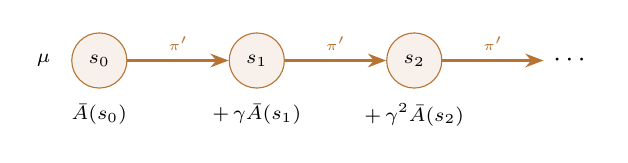
\begin{tikzpicture}[x=2.0cm, >=Stealth,
    st/.style={circle, draw=AtlasWarm, fill=AtlasWarm!10, minimum size=7mm, inner sep=0pt, font=\scriptsize}]
  \node[st] (s0) at (0,0) {$s_0$};
  \node[st] (s1) at (1,0) {$s_1$};
  \node[st] (s2) at (2,0) {$s_2$};
  \node (s3) at (3,0) {$\cdots$};
  \foreach \a/\b in {s0/s1, s1/s2, s2/s3} \draw[->, AtlasWarm, thick] (\a) -- node[above, font=\tiny]{$\pi'$} (\b);
  \node[font=\scriptsize, left=4pt of s0] {$\mu$};
  \node[font=\scriptsize, below=2pt of s0] {$\bar A(s_0)$};
  \node[font=\scriptsize, below=2pt of s1] {$+\,\gamma\bar A(s_1)$};
  \node[font=\scriptsize, below=2pt of s2] {$+\,\gamma^2\bar A(s_2)$};
\end{tikzpicture}
\end{center}

\begin{pair}
\begin{keybox}[title={Exact}]
The gain is the one-step advantages, collected along the \textbf{new} policy's path.
\end{keybox}
\begin{warnbox}[title={Not measurable}]
It needs $d_{\pi',\mu}$: the states of a policy we have not run yet.
\end{warnbox}
\end{pair}

\textbf{Proof sketch.}
\begin{enumerate}
  \item Along a trajectory of $\pi'$, add and subtract $V_\pi(s_t)$ at each step.
  \item The terms $\gamma V_\pi(s_{t+1})-V_\pi(s_t)$ telescope to $-V_\pi(s_0)$.
  \item What remains is $\sum_t\gamma^t A_\pi(s_t,a_t)$; average over $a_t\sim\pi'$.
\end{enumerate}
In operator form, $\bar A(s)=(T_{\pi'}V_\pi)(s)-V_\pi(s)$: what we gain by deviating to $\pi'$ for one step at $s$. This is also the starting point of TRPO (its Eq.~1).

% ---------------------------------------------------------------------------
\section{The policy advantage}
\label{sec:pa}
% ---------------------------------------------------------------------------

\begin{defbox}{policy advantage (K\&L Sec.~4.1)}
\begin{gather*}
  \PA_{\pi,\mu}(\pi') = \E_{s\sim d_{\pi,\mu}}\Big[\E_{a\sim\pi'(\cdot;s)}\big[A_\pi(s,a)\big]\Big] = \E_{s\sim d_{\pi,\mu}}\big[\bar A(s)\big]
\end{gather*}
\end{defbox}

\begin{enumerate}
  \item Lemma 6.1's average, but on the states the \textbf{old} $\pi$ visits (from $\mu$) $\Rightarrow$ \textbf{measurable}.
  \item One step of policy improvement maximizes it.
  \item It is exactly the \textbf{first-order} change of $\eta_\mu$ in $\alpha$ (proof: App.~\ref{app:proof-pa}):
  \begin{gather*}
    \left.\frac{\partial \eta_\mu}{\partial \alpha}\right|_{\alpha=0} = \frac{1}{1-\gamma}\PA_{\pi,\mu}(\pi')
    \qquad\Longrightarrow\qquad
    \Delta\eta_\mu = \frac{\alpha}{1-\gamma}\PA_{\pi,\mu}(\pi') + O(\alpha^2)
  \end{gather*}
\end{enumerate}

\begin{keybox}
Small $\alpha$ + positive policy advantage $\Rightarrow$ improvement. Large $\alpha$ $\Rightarrow$ possible degradation. \textbf{How large can $\alpha$ be?}\\
For TRPO: a surrogate built on the \emph{old} state distribution matches the true objective to first order.
\end{keybox}

\subsection{The exact change vs.\ the policy advantage}

Apply Lemma 6.1 to the mixture $\pinew=(1-\alpha)\pi+\alpha\pi'$. Per state,
$\E_{a\sim\pinew}A_\pi(s,a)=(1-\alpha)\cdot0+\alpha\bar A(s)=\alpha\bar A(s)$. Then add and subtract the old distribution:
\begin{gather*}
  (1-\gamma)\big(\eta_\mu(\pinew)-\eta_\mu(\pi)\big) = \alpha\textstyle\sum_s d_{\pinew,\mu}(s)\,\bar A(s) \\
  = \underbrace{\alpha\textstyle\sum_s d_{\pi,\mu}(s)\,\bar A(s)}_{=\,\alpha\PA:\ \text{old states, measurable}}
    + \underbrace{\alpha\textstyle\sum_s \big(d_{\pinew,\mu}-d_{\pi,\mu}\big)(s)\,\bar A(s)}_{\text{gap: state shift, not measurable}}
\end{gather*}

\begin{minipage}[c]{0.45\linewidth}
\centering
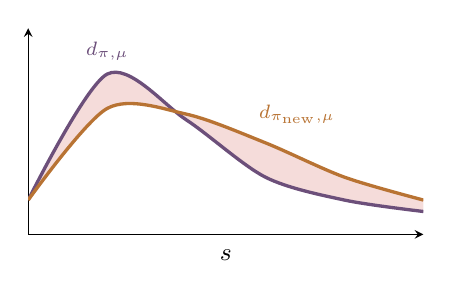
\begin{tikzpicture}
\begin{axis}[notes, width=6.6cm, height=4.2cm, xmin=0, xmax=5, ymin=0, ymax=1.8, xtick=\empty, ytick=\empty, xlabel={$s$}]
  \addplot[name path=old, AtlasSlate, very thick, smooth] coordinates {(0,0.3)(1,1.4)(2,1.0)(3,0.5)(4,0.3)(5,0.2)};
  \addplot[name path=new, AtlasWarm, very thick, smooth] coordinates {(0,0.3)(1,1.1)(2,1.05)(3,0.8)(4,0.5)(5,0.3)};
  \addplot[BadRed!18] fill between[of=old and new];
  \node[AtlasSlate, font=\scriptsize] at (axis cs:1.0,1.6) {$d_{\pi,\mu}$};
  \node[AtlasWarm, font=\scriptsize] at (axis cs:3.4,1.05) {$d_{\pinew,\mu}$};
\end{axis}
\end{tikzpicture}\\
{\scriptsize \textcolor{BadRed}{shaded}: the shift --- $\bar A$ unknown there.}
\end{minipage}\hfill
\begin{minipage}[c]{0.52\linewidth}
\begin{itemize}
  \item $\alpha\PA$: the first-order term above.
  \item Gap: \textbf{two factors of $\alpha$} --- a smaller $\bar A$ \emph{and} less shift ($\pinew$ deviates from $\pi$ only w.p.\ $\alpha$ per step) $\Rightarrow$ $O(\alpha^2)$.
  \item Thm.~4.1 is a \textbf{lower bound on the gap}: a worst case on the shaded mass.
\end{itemize}
\end{minipage}

\begin{keybox}
Exact but unmeasurable (Lemma 6.1) \ $=$ \ measurable ($\alpha\PA$) \ $+$ \ gap. We only need to \textbf{bound the gap}.
\end{keybox}

% ---------------------------------------------------------------------------
\section{How big a step? The improvement bound}
% ---------------------------------------------------------------------------

\begin{thmbox}{Theorem 4.1 (K\&L)}
With $\varepsilon = \max_s \big|\E_{a\sim\pi'}[A_\pi(s,a)]\big|$, for all $\alpha\in[0,1]$:
\begin{gather*}
  \eta_\mu(\pinew) - \eta_\mu(\pi) \;\ge\; \frac{\alpha}{1-\gamma}\Big(\PA - \frac{2\alpha\gamma\varepsilon}{1-\gamma(1-\alpha)}\Big)
\end{gather*}
\end{thmbox}

\begin{minipage}[c]{0.5\linewidth}
\centering
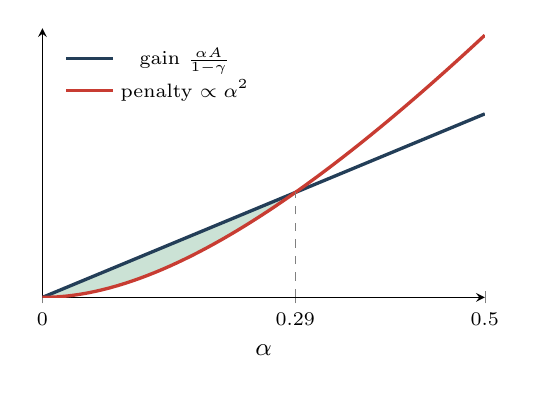
\begin{tikzpicture}
\begin{axis}[notes, width=7.2cm, height=5cm, xmin=0, xmax=0.5, ymin=0, ymax=1.1,
    xlabel={$\alpha$}, xtick={0,0.2857,0.5}, xticklabels={0,0.29,0.5}, ytick=\empty,
    legend pos=north west]
  \addplot[name path=gain, AtlasCool, very thick, domain=0:0.5, samples=60] {1.5*x};
  \addlegendentry{gain $\frac{\alpha\PA}{1-\gamma}$}
  \addplot[name path=pen, BadRed, very thick, domain=0:0.5, samples=60] {3*x^2/(0.4+0.6*x)};
  \addlegendentry{penalty $\propto\alpha^2$}
  \addplot[GoodGreen!25] fill between[of=gain and pen, soft clip={domain=0:0.2857}];
  \draw[dashed, gray] (axis cs:0.2857,0) -- (axis cs:0.2857,0.43);
\end{axis}
\end{tikzpicture}\\
{\scriptsize Illustrative: $\gamma=0.6$, $\varepsilon=1$, $\PA=0.6$. Green: improvement guaranteed.}
\end{minipage}\hfill
\begin{minipage}[c]{0.47\linewidth}
\begin{itemize}
  \item \textbf{Gain} $\alpha\PA$: linear, measured on old states.
  \item \textbf{Penalty}: worst case of the state shift, $\propto\alpha^2$ near 0.
  \item \textbf{Small $\alpha$}: the gain wins $\Rightarrow$ guaranteed progress whenever $\PA>0$.
  \item \textbf{$\alpha=1$}: the B\&T penalty plus a gain; usually loses (needs $\gamma<\frac12$). Comparison: App.~\ref{app:bt}.
\end{itemize}
\end{minipage}

\subsection{Choosing the step: Corollary 4.2}

Three steps.

\textbf{Step 1 --- simplify.} Lower the bound further so that only the measurable $\PA$ is left. Use $\varepsilon\le R$, \ $1-\gamma(1-\alpha)\ge1-\gamma$, \ $\gamma\le1$:
\begin{gather*}
  \eta_\mu(\pinew)-\eta_\mu(\pi) \;\ge\; \frac{\alpha}{1-\gamma}\Big(\PA - \frac{2\alpha R}{1-\gamma}\Big) \;=:\; f(\alpha)
\end{gather*}

\textbf{Step 2 --- maximize.} $f(\alpha)=\frac{\PA}{1-\gamma}\alpha-\frac{2R}{(1-\gamma)^2}\alpha^2$ is a downward parabola:
\begin{gather*}
  f'(\alpha) = \frac{\PA}{1-\gamma} - \frac{4R\,\alpha}{(1-\gamma)^2} = 0
  \quad\Longrightarrow\quad
  \alpha^* = \frac{(1-\gamma)\PA}{4R}
\end{gather*}

\textbf{Step 3 --- plug in.}
\begin{gather*}
  f(\alpha^*) = \frac{\PA}{1-\gamma}\cdot\frac{(1-\gamma)\PA}{4R} - \frac{2R}{(1-\gamma)^2}\cdot\frac{(1-\gamma)^2\PA^2}{16R^2}
  = \frac{\PA^2}{4R}-\frac{\PA^2}{8R} = \frac{\PA^2}{8R}
\end{gather*}

\begin{minipage}[c]{0.48\linewidth}
\begin{thmbox}{Corollary 4.2}
If $\PA\ge0$, then $\alpha=\frac{(1-\gamma)\PA}{4R}$ guarantees
\begin{gather*}
  \eta_\mu(\pinew)-\eta_\mu(\pi)\ge\frac{\PA^2}{8R}.
\end{gather*}
\end{thmbox}
\end{minipage}\hfill
\begin{minipage}[c]{0.48\linewidth}
\centering
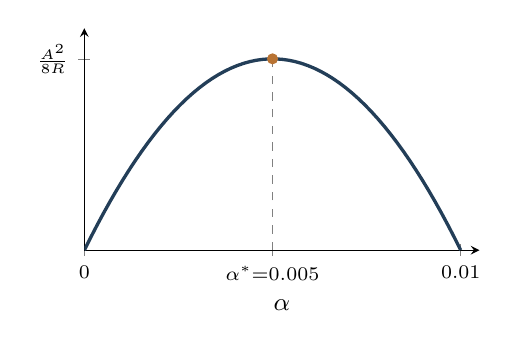
\begin{tikzpicture}
\begin{axis}[notes, width=6.6cm, height=4.4cm, xmin=0, xmax=0.0105, ymin=0, ymax=0.0058,
    xlabel={$\alpha$}, xtick={0,0.005,0.01}, xticklabels={0,$\alpha^*{=}0.005$,0.01},
    ytick={0.005}, yticklabels={$\frac{\PA^2}{8R}$}, scaled ticks=false]
  \addplot[AtlasCool, very thick, domain=0:0.01, samples=60] {2*x-200*x^2};
  \draw[dashed, gray] (axis cs:0.005,0) -- (axis cs:0.005,0.005);
  \fill[AtlasWarm] (axis cs:0.005,0.005) circle (2pt);
\end{axis}
\end{tikzpicture}\\
{\scriptsize $f(\alpha)$ for $\gamma=0.9$, $R=1$, $\PA=0.2$.}
\end{minipage}

\begin{pair}
\begin{keybox}[title={Computable}]
$\PA$ averages over the \emph{old} policy's states ($\mu$-restarts); $R$ is known. The unknown $\varepsilon$ (a max over all states) is gone.
\end{keybox}
\begin{warnbox}[title={Tiny steps}]
$\PA\le R$ gives $\alpha\le(1-\gamma)/4$ \ (${}\le0.0025$ at $\gamma=0.99$), and $\alpha\to0$ as $\PA\to0$. This worst-case conservatism is what TRPO relaxes.
\end{warnbox}
\end{pair}

% ---------------------------------------------------------------------------
\section{The CPI algorithm}
\label{sec:cpi-alg}
% ---------------------------------------------------------------------------

\begin{algbox}{Conservative Policy Iteration}
\begin{enumerate}
  \item $\pi' \leftarrow G_\varepsilon(\pi,\mu)$ \hfill {\small(greedy policy chooser)}
  \item Estimate $\hat\PA \approx \PA_{\pi,\mu}(\pi')$ to $\pm\frac\varepsilon3$ with $O\big(\frac{R^2}{\varepsilon^2}\log\frac{R^2}{\delta\varepsilon^2}\big)$ $\mu$-restarts.
  \item If $\hat\PA < \frac{2\varepsilon}{3}$: \textbf{stop}, return $\pi$.
  \item Else: mix with $\alpha = \frac{(1-\gamma)(\hat\PA - \varepsilon/3)}{4R}$, and go to 1.
\end{enumerate}
\end{algbox}

\begin{defbox}{greedy policy chooser $G_\varepsilon$ and $\OPT$}
$G_\varepsilon(\pi,\mu)$ returns $\pi'$ with $\PA_{\pi,\mu}(\pi') \ge \OPT(\PA_{\pi,\mu}) - \varepsilon$, where
\begin{gather*}
  \OPT(\PA_{\pi,\mu}) \equiv \max_{\pi'}\PA_{\pi,\mu}(\pi') = \E_{s\sim d_{\pi,\mu}}\big[\max_a A_\pi(s,a)\big]
\end{gather*}
is the largest policy advantage any $\pi'$ can achieve (Def.~4.3). Small $\OPT$ $\Rightarrow$ no policy improves much on $\pi$ under $d_{\pi,\mu}$. One way to build $G_\varepsilon$: a regression on advantages with \textbf{average} error $\le\varepsilon/2$ (App.~\ref{app:greedy}).
\end{defbox}

\begin{thmbox}{Theorem 4.4 (K\&L)}
With probability $\ge1-\delta$, CPI:
\begin{enumerate}[label=\roman*)]
  \item improves $\eta_\mu$ at \textbf{every} update;
  \item stops within $72\,R^2/\varepsilon^2$ calls to $G_\varepsilon$;
  \item returns $\pi$ with $\OPT(\PA_{\pi,\mu}) < 2\varepsilon$.
\end{enumerate}
\end{thmbox}

\begin{notebox}
Why at most $72R^2/\varepsilon^2$ updates: each update gains $\ge\PA^2/8R\ge\varepsilon^2/(72R)$ (since $\PA\ge\varepsilon/3$ when CPI steps), and $\eta_\mu\le R$. The count does \textbf{not} depend on $\mu$ or on the size of the state space.
\end{notebox}

\subsection{Verifying an update: estimating $\PA$ from $\mu$-restarts}

Since $V_\pi(s)=\sum_a\pi(a;s)\,Q_\pi(s,a)$, the policy advantage needs only $Q_\pi$:
\begin{gather*}
  \PA_{\pi,\mu}(\pi') = \E_{s\sim d_{\pi,\mu}}\Big[\textstyle\sum_a\big(\pi'(a;s)-\pi(a;s)\big)\,Q_\pi(s,a)\Big]
\end{gather*}

\begin{center}
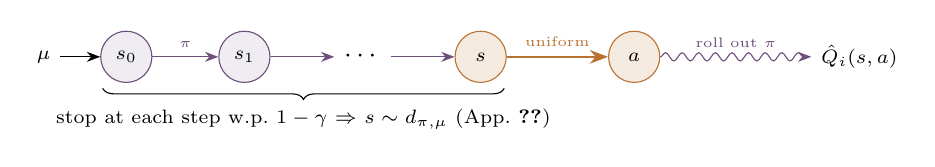
\begin{tikzpicture}[x=1.5cm, >=Stealth,
    st/.style={circle, draw=AtlasSlate, fill=AtlasSlate!10, minimum size=6.5mm, inner sep=0pt, font=\scriptsize}]
  \node[font=\scriptsize] (mu) at (-0.7,0) {$\mu$};
  \node[st] (s0) at (0,0) {$s_0$};
  \node[st] (s1) at (1,0) {$s_1$};
  \node (dd) at (2,0) {$\cdots$};
  \node[st, draw=AtlasWarm, fill=AtlasWarm!15] (s) at (3,0) {$s$};
  \draw[->] (mu) -- (s0);
  \draw[->, AtlasSlate] (s0) -- node[above, font=\tiny]{$\pi$} (s1);
  \draw[->, AtlasSlate] (s1) -- (dd);
  \draw[->, AtlasSlate] (dd) -- (s);
  \draw[decorate, decoration={brace, amplitude=4pt, mirror}] (-0.2,-0.4) -- node[below=4pt, font=\scriptsize]{stop at each step w.p.\ $1-\gamma$ $\Rightarrow$ $s\sim d_{\pi,\mu}$ (App.~\ref{app:geom})} (3.2,-0.4);
  \node[st, draw=AtlasWarm, fill=AtlasWarm!15] (a) at (4.3,0) {$a$};
  \draw[->, AtlasWarm, thick] (s) -- node[above, font=\tiny]{uniform} (a);
  \node[font=\scriptsize, right] (q) at (5.8,0) {$\hat Q_i(s,a)$};
  \draw[->, AtlasSlate, decorate, decoration={snake, amplitude=1.5pt, segment length=6pt}] (a) -- node[above, font=\tiny]{roll out $\pi$} (q);
\end{tikzpicture}
\end{center}

\begin{eqbox}
\begin{gather*}
  x_i = n_a\,\hat Q_i(s,a)\big(\pi'(a;s)-\pi(a;s)\big)\in[-n_aR,\,n_aR], \qquad \hat\PA=\tfrac1k\textstyle\sum_{i=1}^k x_i\\
  \text{Hoeffding:}\quad \Pr\big(|\hat\PA-\PA|>\Delta\big) \;\le\; 2\,e^{-k\Delta^2/(2n_a^2R^2)}
\end{gather*}
\end{eqbox}

\begin{enumerate}
  \item \textbf{Unbiased:} $a$ uniform $\Rightarrow$ $\E_a[n_af(a)]=\sum_af(a)$. An importance weight $n_a$ (the number of actions) --- App.~\ref{app:is-cpi}, App.~\ref{app:hoeffding}.
  \item \textbf{Only rollouts of the current $\pi$} --- no need to run $\pinew$. \textbf{This is the answer to Q2.}
  \item CPI uses $\Delta=\varepsilon/3$, so $\hat\PA-\frac\varepsilon3\le\PA$ is safe for the stop test and for $\alpha$.
\end{enumerate}

\begin{center}
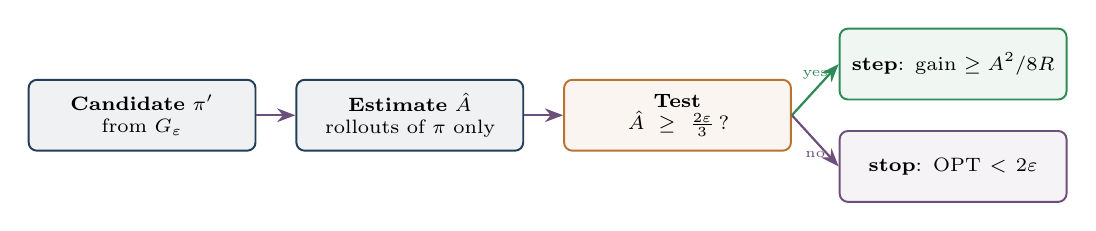
\begin{tikzpicture}[>=Stealth, box/.style={fl, font=\scriptsize, minimum height=0.9cm, text width=2.6cm}]
  \node[box, cbox=AtlasCool] (prop) at (0,0) {\textbf{Candidate} $\pi'$\\from $G_\varepsilon$};
  \node[box, cbox=AtlasCool] (est) at (3.4,0) {\textbf{Estimate} $\hat\PA$\\rollouts of $\pi$ only};
  \node[box, cbox=AtlasWarm] (test) at (6.8,0) {\textbf{Test}\\$\hat\PA\ge\frac{2\varepsilon}{3}$\,?};
  \node[box, cbox=GoodGreen] (yes) at (10.3,0.65) {\textbf{step}: gain $\ge\PA^2/8R$};
  \node[box, cbox=AtlasSlate] (no) at (10.3,-0.65) {\textbf{stop}: $\OPT<2\varepsilon$};
  \draw[->, thick, AtlasSlate] (prop) -- (est);
  \draw[->, thick, AtlasSlate] (est) -- (test);
  \draw[->, thick, GoodGreen] (test.east) -- node[above, font=\tiny]{yes} (yes.west);
  \draw[->, thick, AtlasSlate] (test.east) -- node[below, font=\tiny]{no} (no.west);
\end{tikzpicture}
\end{center}

\begin{notebox}
\textbf{The naive check} --- run $\pi'$ and compare returns --- is noisy and needs rollouts of the \textbf{new} policy ($d_{\pi',\mu}$, Lemma~6.1). CPI tests \emph{before} stepping, with data from the current policy only.
\end{notebox}

% ---------------------------------------------------------------------------
\section{How good is the policy found?}
% ---------------------------------------------------------------------------

\begin{thmbox}{Theorem 6.2 (K\&L)}
If $\OPT(\PA_{\pi,\mu}) < \varepsilon$, then for any $\tilde\mu$:
\begin{gather*}
  \eta_{\tilde\mu}(\pi^*) - \eta_{\tilde\mu}(\pi)
  \;\le\; \frac{\varepsilon}{1-\gamma}\left\|\frac{d_{\pi^*,\tilde\mu}}{d_{\pi,\mu}}\right\|_\infty
  \;\le\; \frac{\varepsilon}{(1-\gamma)^2}\left\|\frac{d_{\pi^*,\tilde\mu}}{\mu}\right\|_\infty
\end{gather*}
With $\tilde\mu=D$ this bounds the real goal $\eta_D$ (Cor.~4.5).
\end{thmbox}

\textbf{Proof in three steps.}
\begin{enumerate}
  \item Lemma 6.1 for $\pi^*$ vs.\ $\pi$: \ $\eta(\pi^*)-\eta(\pi)=\frac{1}{1-\gamma}\E_{d_{\pi^*,\tilde\mu}}\big[\E_{a\sim\pi^*}A_\pi\big]$.
  \item $\E_{a\sim\pi^*}[A_\pi]\le\max_aA_\pi$, which is $\ge0$ (since $\E_{a\sim\pi}A_\pi=0$).
  \item Change of measure: $\E_p[f]\le\|p/q\|_\infty\E_q[f]$ for $f\ge0$, with $\E_{d_{\pi,\mu}}[\max_aA_\pi]=\OPT(\PA_{\pi,\mu})<\varepsilon$.
\end{enumerate}

\begin{pair}
\begin{coolbox}[title={A covariate-shift bound}]
\small test risk $\le$ density ratio $\times$ train risk
\begin{itemize}
  \item train risk: $\OPT(\PA_{\pi,\mu})$, on CPI's data $d_{\pi,\mu}$
  \item test: the states $\pi^*$ visits, $d_{\pi^*,\tilde\mu}$
\end{itemize}
\end{coolbox}
\begin{keybox}[title={Uniform $\mu$ caps the ratio}]
\small $d_{\pi,\mu}\ge(1-\gamma)\mu$, so with uniform $\mu$ the ratio is $\le|S|/(1-\gamma)$ --- for \textbf{any} $\pi^*$. Later RL theory calls it the \emph{concentrability coefficient}.
\end{keybox}
\end{pair}

{\small Two factors of $\frac1{1-\gamma}$: one from the lemma, one from $d_{\pi,\mu}\ge(1-\gamma)\mu$. Sec.~7.3 of the paper: choose $\mu$ using prior knowledge of where an optimal policy goes.}

% ---------------------------------------------------------------------------
\section{Summary of Part I}
% ---------------------------------------------------------------------------

\begin{tcolorbox}[notes, colback=GoodGreen!5, colframe=GoodGreen, colbacktitle=GoodGreen, title={CPI's answers to the three questions}]
\begin{enumerate}[label=\textbf{Q\arabic*}]
  \item \textbf{Improving measure:} $\eta_\mu$ improves at every update (Thm.~4.4).
  \item \textbf{Verification:} estimate the policy advantage $\PA$ from samples of the current policy (Hoeffding).
  \item \textbf{Performance:} within $O(R^2/\varepsilon^2)$ updates, close to optimal up to the mismatch factor (Thm.~6.2).
\end{enumerate}
\end{tcolorbox}

\begin{pair}
\begin{keybox}[title={Kept going forward}]
\begin{itemize}
  \item Surrogate on the \textbf{old} state distribution
  \item Improvement lower bound $=$ gain $-$ penalty
  \item Small, controlled steps
\end{itemize}
\end{keybox}
\begin{warnbox}[title={Limitations}]
\begin{itemize}
  \item Only \textbf{mixture} policies
  \item Needs a restart distribution
  \item Theoretical step sizes are tiny
\end{itemize}
\end{warnbox}
\end{pair}

\begin{notebox}
Like non-convex SGD (a bounded objective and a sure gain per step $\Rightarrow$ few steps to a stationary point), but Thm.~6.2 turns ``stationary'' into ``near-optimal''. Details: App.~\ref{app:cpi-sgd}.
\end{notebox}

\subsection{The two lanes to follow}

\begin{center}
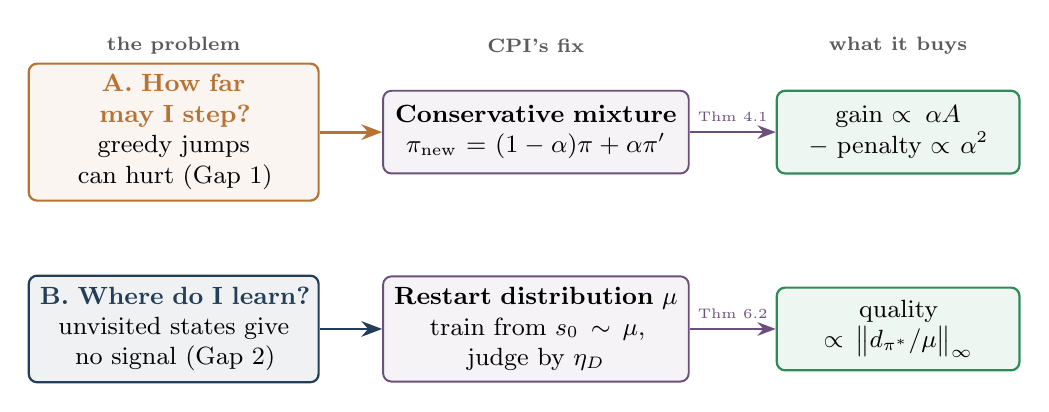
\begin{tikzpicture}[font=\footnotesize, >=Stealth,
    fix/.style={fl, line width=0.8pt, text width=3.4cm, minimum height=1.1cm},
    res/.style={fl, cbox=AtlasSlate, text width=3.6cm, minimum height=1.05cm},
    q/.style={fl, draw=GoodGreen, fill=GoodGreen!8, line width=0.8pt, text width=2.8cm, minimum height=1.05cm}]
  \node[font=\scriptsize\bfseries, NoteGray] at (0,2.6) {the problem};
  \node[font=\scriptsize\bfseries, NoteGray] at (4.6,2.6) {CPI's fix};
  \node[font=\scriptsize\bfseries, NoteGray] at (9.2,2.6) {what it buys};
  \node[fix, cbox=AtlasWarm] (pa) at (0,1.5) {\textbf{\color{AtlasWarm}A. How far may I step?}\\ greedy jumps can hurt (Gap 1)};
  \node[res] (fa) at (4.6,1.5) {\textbf{Conservative mixture}\\ $\pinew=(1-\alpha)\pi+\alpha\pi'$};
  \node[q] (ra) at (9.2,1.5) {gain $\propto\alpha\PA$\\ $-$ penalty $\propto\alpha^2$};
  \node[fix, cbox=AtlasCool] (pb) at (0,-1.0) {\textbf{\color{AtlasCool}B. Where do I learn?}\\ unvisited states give no signal (Gap 2)};
  \node[res] (fb) at (4.6,-1.0) {\textbf{Restart distribution $\mu$}\\ train from $s_0\sim\mu$, judge by $\eta_D$};
  \node[q] (rb) at (9.2,-1.0) {quality $\propto\big\|d_{\pi^*}/\mu\big\|_\infty$};
  \draw[->, line width=1pt, AtlasWarm] (pa) -- (fa);
  \draw[->, AtlasSlate, thick] (fa) -- node[above, font=\tiny]{Thm 4.1} (ra);
  \draw[->, line width=1pt, AtlasCool] (pb) -- (fb);
  \draw[->, AtlasSlate, thick] (fb) -- node[above, font=\tiny]{Thm 6.2} (rb);
\end{tikzpicture}
\end{center}

\begin{keybox}
Two \textbf{separate} axes: \textbf{update size} (A) and \textbf{state coverage} (B). TRPO keeps lane A and drops lane B; GAE and PPO never bring B back.
\end{keybox}

% ===========================================================================
%  PART II --- TRUST REGION POLICY OPTIMIZATION (Schulman et al., 2015)
% ===========================================================================
\clearpage
\part{Trust Region Policy Optimization}

\partintro{\textbf{The question of Part II:} CPI's guarantee only holds for \emph{mixture} policies. TRPO replaces the mixing weight $\alpha$ by a \textbf{distance between policies}, gets a monotone-improvement bound for \textbf{any} stochastic policy $\pi_\theta$, and then makes it practical in \textbf{five simplifications}. It keeps lane A of CPI and drops lane B.}

% ---------------------------------------------------------------------------
\section{Setting: what changes from CPI}
% ---------------------------------------------------------------------------

\paper{Trust Region Policy Optimization}
  {Schulman, Levine, Moritz, Jordan \& Abbeel}{ICML 2015}
  {TRPO --- CPI's guarantee for any stochastic policy $\pi_\theta$}
  {trust\_region\_policy\_optimization.md}

An MDP $(\mathcal{S}, \mathcal{A}, P, r, \rho_0, \gamma)$:

\begin{enumerate}
  \item \textbf{Finite} $\mathcal{S},\mathcal{A}$ in the proofs --- also holds for \textbf{continuous} spaces (conditions in App.~\ref{app:trpo-cont}).
  \item \textbf{Discounted}: $\gamma\in(0,1)$, reward $r(s)$.
  \item \textbf{Unknown dynamics}: sample trajectories only.
  \item \textbf{Start distribution} $\rho_0$ (CPI's $D$) --- {\color{BadRed}\textbf{no restart distribution $\mu$}}.
  \item \textbf{Unnormalized}: $\eta(\pi)=\E\big[\sum_t\gamma^t r(s_t)\big]$, $s_0\sim\rho_0$.
  \item \textbf{Any} differentiable stochastic policy $\pi_\theta$ (e.g.\ a neural net).
\end{enumerate}

\begin{minipage}[c]{0.56\linewidth}
\small
\begin{tabular}{@{}l l l@{}}
\toprule
 & \textbf{\color{AtlasWarm}CPI} & \textbf{\color{AtlasCool}TRPO} \\
\midrule
policies & mixtures $\pi_\alpha$ & any $\pi_\theta$ \\
new candidate & greedy chooser $G_\varepsilon$ & a step in $\theta$ \\
``how far'' & weight $\alpha$ & distance $D(\piold,\pinew)$ \\
start states & $D$, trained from $\mu$ & $\rho_0$ only \\
scale & normalized by $1-\gamma$ & unnormalized \\
\bottomrule
\end{tabular}
\end{minipage}\hfill
\begin{minipage}[c]{0.4\linewidth}
\centering
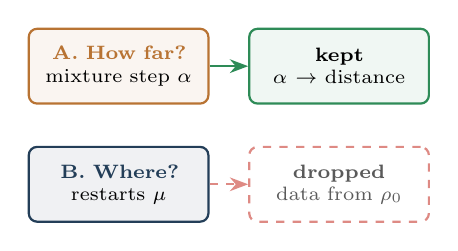
\begin{tikzpicture}[font=\scriptsize, >=Stealth,
    ln/.style={fl, line width=0.8pt, text width=2.0cm, minimum height=0.95cm, font=\scriptsize}]
  \node[ln, cbox=AtlasWarm] (a) at (0,1.3) {\textbf{\color{AtlasWarm}A. How far?}\\ mixture step $\alpha$};
  \node[ln, cbox=AtlasCool] (b) at (0,-0.2) {\textbf{\color{AtlasCool}B. Where?}\\ restarts $\mu$};
  \node[ln, cbox=GoodGreen] (a2) at (2.8,1.3) {\textbf{kept}\\ $\alpha\to$ distance};
  \node[ln, draw=BadRed!60, dashed, text=NoteGray] (b2) at (2.8,-0.2) {\textbf{dropped}\\ data from $\rho_0$};
  \draw[->, thick, GoodGreen] (a) -- (a2);
  \draw[->, thick, BadRed!60, dashed] (b) -- (b2);
\end{tikzpicture}
\end{minipage}

\begin{warnbox}[title={Lane B is dropped}]
The only resets in TRPO are in the ``vine'' scheme (\S\ref{sec:trpo-sampling}), and they go to states \emph{already reached} from $\rho_0$ --- not an exploratory $\mu$. We return to this in \S\ref{sec:trpo-noexplore}.
\end{warnbox}

\textbf{Roadmap of the part:} same identity $\to$ Theorem 1 (any policy) $\to$ KL and MM $\to$ five practical simplifications $\to$ the algorithm.

% ---------------------------------------------------------------------------
\section{The same identity, a local surrogate}
% ---------------------------------------------------------------------------

Unnormalized return and visitation:
\begin{gather*}
  \eta(\pi)=\E\Big[\textstyle\sum_t\gamma^t r(s_t)\Big], \qquad \rho_\pi(s)=\textstyle\sum_t\gamma^t P(s_t=s).
\end{gather*}

\begin{thmbox}{Performance difference (TRPO Eq.~2 = K\&L Lemma 6.1)}
\begin{gather*}
  \eta(\tilde\pi) = \eta(\pi) + \sum_s \rho_{\tilde\pi}(s) \sum_a \tilde\pi(a\mid s)\, A_\pi(s,a)
\end{gather*}
\end{thmbox}

$\rho_{\tilde\pi}$ depends on $\tilde\pi$ in a complicated way $\Rightarrow$ replace it by the \textbf{old} visitation:

\begin{defbox}{local surrogate $L_\pi$ (TRPO Eq.~3)}
\begin{gather*}
  L_\pi(\tilde\pi) = \eta(\pi) + \sum_s \rho_{\pi}(s) \sum_a \tilde\pi(a\mid s)\, A_\pi(s,a)
\end{gather*}
\end{defbox}

\begin{pair}
\begin{keybox}[title={Matches $\eta$ to first order}]
$L_{\pi_{\theta_0}}(\pi_{\theta_0}) = \eta(\pi_{\theta_0})$ and the gradients are equal at $\theta_0$. The same idea as CPI's policy advantage, now for any $\theta$.
\end{keybox}
\begin{warnbox}[title={Says nothing about step size}]
First-order agreement says a \emph{small enough} step helps --- not \textbf{how big} a step is safe.
\end{warnbox}
\end{pair}

\begin{notebox}
TRPO restates CPI's bound (slightly weakened): $\eta(\pinew)\ge L_{\piold}(\pinew)-\frac{2\epsilon\gamma}{(1-\gamma)^2}\alpha^2$ with $\epsilon=\max_s|\E_{a\sim\pi'}A_\pi(s,a)|$ --- valid only for mixtures. Why the first-order statement holds for any parameterization: App.~\ref{app:proof-pa} (the proof never uses that $\alpha$ is a mixing weight).
\end{notebox}

% ---------------------------------------------------------------------------
\section{From mixtures to any stochastic policy: Theorem 1}
% ---------------------------------------------------------------------------

Replace the mixing weight $\alpha$ by the \textbf{total variation distance}:

\begin{defbox}{total variation, max over states}
\begin{gather*}
  \DTV(p\,\|\,q)=\tfrac12\textstyle\sum_a\big|p(a)-q(a)\big|, \qquad
  \DTV^{\max}(\pi,\tilde\pi) = \max_s \DTV\big(\pi(\cdot\mid s)\,\|\,\tilde\pi(\cdot\mid s)\big)
\end{gather*}
\end{defbox}

\begin{minipage}[c]{0.48\linewidth}
\centering
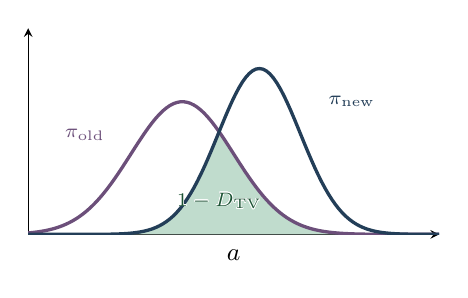
\begin{tikzpicture}
\begin{axis}[notes, width=6.8cm, height=4.2cm, xmin=-3, xmax=5, ymin=0, ymax=0.62, xtick=\empty, ytick=\empty, xlabel={$a$}]
  \addplot[fill=GoodGreen!30, draw=none, domain=-3:5, samples=120]
    {min(exp(-x^2/2)/sqrt(2*pi), exp(-(x-1.5)^2/(2*0.64))/(0.8*sqrt(2*pi)))} \closedcycle;
  \addplot[AtlasSlate, very thick, domain=-3:5, samples=120] {exp(-x^2/2)/sqrt(2*pi)};
  \addplot[AtlasCool, very thick, domain=-3:5, samples=120] {exp(-(x-1.5)^2/(2*0.64))/(0.8*sqrt(2*pi))};
  \node[font=\scriptsize, AtlasSlate] at (axis cs:-1.9,0.3) {$\piold$};
  \node[font=\scriptsize, AtlasCool] at (axis cs:3.3,0.4) {$\pinew$};
  \node[font=\scriptsize, GoodGreen!60!black] at (axis cs:0.72,0.1) {\contour{white}{$1-\DTV$}};
\end{axis}
\end{tikzpicture}
\end{minipage}\hfill
\begin{minipage}[c]{0.48\linewidth}
\begin{itemize}
  \item Green area: the \textbf{shared mass} $\sum_a\min(p,q)=1-\DTV$.
  \item \textbf{Coupling}: draw $a\sim\piold$, $\tilde a\sim\pinew$ so that they are \textbf{equal} with probability $1-\DTV$ (maximal coupling).
  \item So the new policy ``acts like the old one'' w.p.\ $1-\alpha$ at each state --- exactly the structure of a CPI mixture.
\end{itemize}
\end{minipage}

\begin{thmbox}{Theorem 1 (TRPO)}
Let $\alpha=\DTV^{\max}(\piold,\pinew)$. Then
\begin{gather*}
  \eta(\pinew) \;\ge\; L_{\piold}(\pinew) - \frac{4\epsilon\gamma}{(1-\gamma)^2}\,\alpha^2,
  \qquad \epsilon = \max_{s,a}|A_\pi(s,a)|
\end{gather*}
\end{thmbox}

\begin{enumerate}
  \item \textbf{Proof idea}: couple the two policies; they agree w.p.\ $1-\alpha$, which is all the CPI proof needs (TRPO App.~A, adapted from K\&L Thm.~4.1; App.~B gives a second proof by perturbation theory).
  \item \textbf{Different $\epsilon$}: a max over $(s,a)$ of $|A_\pi|$, not CPI's max over $s$ of an expectation. How the two relate: App.~\ref{app:bt}.
  \item \textbf{Why a max over states}: the coupling must hold at every state the new policy might reach.
\end{enumerate}

% ---------------------------------------------------------------------------
\section{From TV to KL: a minorize--maximize algorithm}
% ---------------------------------------------------------------------------

\begin{defbox}{KL divergence}
\begin{gather*}
  \DKL(p\|q)=\textstyle\sum_a p(a)\log\frac{p(a)}{q(a)}\ \ge 0 \qquad \text{--- smooth in $\theta$, unlike $\DTV$.}
\end{gather*}
\end{defbox}

Use $\DTV(p\|q)^2\le\DKL(p\|q)$ (Pinsker-type) in Theorem 1:

\begin{eqbox}
\begin{gather*}
  \eta(\tilde\pi) \;\ge\; \underbrace{L_\pi(\tilde\pi) - C\,\DKL^{\max}(\pi,\tilde\pi)}_{M_i(\tilde\pi)},
  \qquad C = \frac{4\epsilon\gamma}{(1-\gamma)^2}
\end{gather*}
\end{eqbox}

\begin{minipage}[c]{0.48\linewidth}
\centering
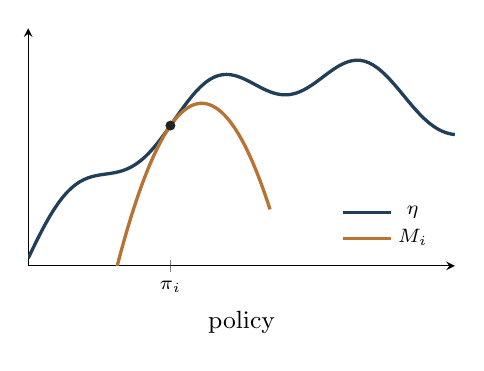
\begin{tikzpicture}
\begin{axis}[notes, width=7cm, height=4.6cm, xmin=0, xmax=6, ymin=0.5, ymax=3.6, xtick={2}, xticklabels={$\pi_i$},
    ytick=\empty, xlabel={policy}, legend pos=south east,
    declare function={eta(\x) = 3 - 0.15*(\x-4)^2 + 0.25*sin(deg(3*\x));
                       etap(\x) = -0.3*(\x-4) + 0.75*cos(deg(3*\x));
                       mm(\x) = eta(2) + etap(2)*(\x-2) - 1.5*(\x-2)^2;}]
  \addplot[AtlasCool, very thick, domain=0:6, samples=100] {eta(x)};
  \addlegendentry{$\eta$}
  \addplot[AtlasWarm, very thick, domain=0.6:3.4, samples=80] {mm(x)};
  \addlegendentry{$M_i$}
  \fill[AtlasInk] (axis cs:2,{eta(2)}) circle (1.8pt);
\end{axis}
\end{tikzpicture}\\
{\scriptsize Illustrative. $M_i$ touches $\eta$ at $\pi_i$ and lies below it.}
\end{minipage}\hfill
\begin{minipage}[c]{0.48\linewidth}
\begin{enumerate}
  \item $M_i\le\eta$ everywhere, with equality at $\pi_i$.
  \item Maximize $M_i$:
  \begin{gather*}
    \eta(\pi_{i+1})-\eta(\pi_i)\ \ge\ M_i(\pi_{i+1})-M_i(\pi_i)\ \ge\ 0.
  \end{gather*}
  \item $\Rightarrow$ \textbf{monotone improvement} (with exact advantages).
\end{enumerate}
{\small MM = minorization--maximization (Hunter \& Lange 2004), the same family as EM.}
\end{minipage}

\begin{keybox}
This penalized problem is what \textbf{the theory covers}. Everything after this point trades a guarantee for practicality.
\end{keybox}

% ---------------------------------------------------------------------------
\section{Five practical simplifications}
% ---------------------------------------------------------------------------

Each simplification is shown with the same three boxes: why it is needed, what changes, and what it costs.

\subsection{1. From penalty to constraint: the trust region}
\trpostep{1}

\begin{pair}
\begin{warmbox}[title={Theory (penalty)}]
\begin{gather*}
  \max_\theta\ L_{\told}(\theta) - C\,\DKL^{\max}(\told,\theta)
\end{gather*}
With the theoretical $C$ the steps are \textbf{tiny}, and a good $C$ is hard to choose robustly.
\end{warmbox}
\begin{coolbox}[title={Practice (constraint)}]
\begin{gather*}
  \max_\theta\ L_{\told}(\theta) \quad \text{s.t.}\ \ \DKL^{\max}(\told,\theta) \le \delta
\end{gather*}
$\delta$ lives in policy space, so it transfers across problems ($\delta=0.01$ in all experiments).
\end{coolbox}
\end{pair}

\simp{$C=\frac{4\epsilon\gamma}{(1-\gamma)^2}$: at $\gamma=0.99$, $C\approx4\cdot10^4\,\epsilon$ $\Rightarrow$ tiny steps.}
     {A hard limit $\delta$ on the KL replaces the penalty $C$: optimize $L$ only where we \emph{trust} it.}
     {The guarantee becomes a heuristic; $\delta$ is a hyperparameter.}

{\small The constraint is the Lagrangian-dual view of the penalty: each $\delta$ corresponds to some $C$.}

\subsection{2. From max KL to mean KL}
\trpostep{2}

Replace the max over states by an average under the old visitation:
\begin{gather*}
  \bar D_{\mathrm{KL}}^{\rho}(\theta_1,\theta_2) = \E_{s\sim\rho}\Big[\DKL\big(\pi_{\theta_1}(\cdot\mid s)\,\|\,\pi_{\theta_2}(\cdot\mid s)\big)\Big]
\end{gather*}
\begin{eqbox}
\begin{gather*}
  \max_\theta\ L_{\told}(\theta) \quad\text{s.t.}\quad \bar D_{\mathrm{KL}}^{\rho_{\told}}(\told,\theta) \le \delta
\end{gather*}
\end{eqbox}

\simp{$\DKL^{\max}$ is one constraint \textbf{per state}, also at states we never sample.}
     {An \textbf{expectation} over visited states $\Rightarrow$ estimated from the same rollouts.}
     {Rarely visited states may change a lot. Empirically close to max KL (cart-pole, \S\ref{sec:trpo-results}).}

\subsection{Tool: importance sampling}
\label{sec:is-trpo}

\begin{enumerate}
  \item \textbf{Monte Carlo:} an expectation $\approx$ an average of samples, $\E_{a\sim p}[f]\approx\frac1n\sum_i f(a_i)$, $a_i\sim p$.
  \item \textbf{Samples only from $q$?} Weight by $w=p/q$ (needs $q>0$ where $p>0$):
  \begin{gather*}
    \E_{a\sim p}[f] = \textstyle\sum_a q\,\frac{p}{q}\,f = \E_{a\sim q}\big[w\,f\big]
  \end{gather*}
  \item \textbf{Unbiased for any $q$; the variance depends on $q$:}
  \begin{gather*}
    \hat\mu = \tfrac1n\textstyle\sum_{i} w(a_i)\,f(a_i), \qquad \mathrm{Var}[\hat\mu] = \tfrac1n\mathrm{Var}_{q}\big[w f\big]
  \end{gather*}
  \item \textbf{In TRPO} (single path), at each state $s$: $p=\pi_\theta(\cdot\mid s)$, $q=\pi_{\told}(\cdot\mid s)$, \ $w=\frac{\pi_\theta(a\mid s)}{\pi_{\told}(a\mid s)}$.
\end{enumerate}

\begin{center}
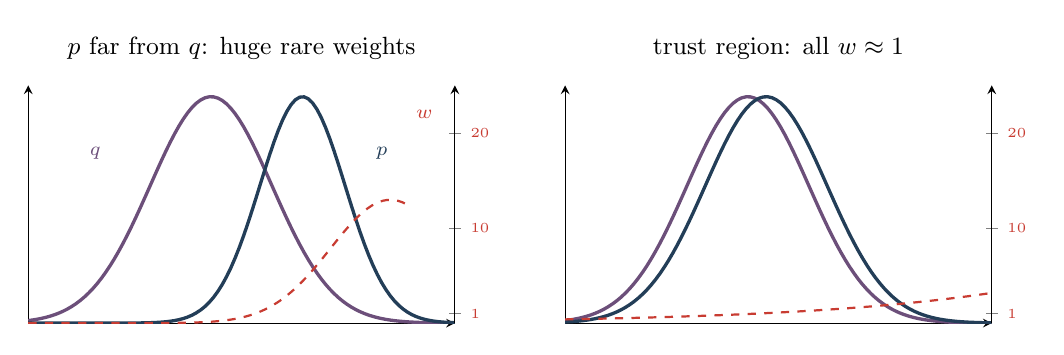
\begin{tikzpicture}
\begin{axis}[notes, name=far, width=7cm, height=4.6cm, xmin=-3, xmax=4, ymin=0, ymax=1.05, xtick=\empty, ytick=\empty,
    title={\small $p$ far from $q$: huge rare weights}, axis y line*=left]
  \addplot[AtlasSlate, very thick, domain=-3:4, samples=100] {exp(-x^2/2)};
  \addplot[AtlasCool, very thick, domain=-3:4, samples=100] {exp(-(x-1.5)^2/(2*0.49))};
  \node[font=\scriptsize, AtlasSlate] at (axis cs:-1.9,0.75) {$q$};
  \node[font=\scriptsize, AtlasCool] at (axis cs:2.8,0.75) {$p$};
\end{axis}
\begin{axis}[notes, at={(far.south west)}, anchor=south west, width=7cm, height=4.6cm, xmin=-3, xmax=4, ymin=0, ymax=25,
    axis x line=none, axis y line*=right, ytick={1,10,20}, yticklabel style={font=\tiny, BadRed}]
  \addplot[BadRed, thick, dashed, domain=-3:3.2, samples=100] {exp(-(x-1.5)^2/(2*0.49) + x^2/2)/0.7};
  \node[font=\scriptsize, BadRed] at (axis cs:3.5,22) {$w$};
\end{axis}
\begin{axis}[notes, name=near, at={(far.east)}, anchor=west, xshift=1.4cm, width=7cm, height=4.6cm, xmin=-3, xmax=4, ymin=0, ymax=1.05,
    xtick=\empty, ytick=\empty, title={\small trust region: all $w\approx1$}, axis y line*=left]
  \addplot[AtlasSlate, very thick, domain=-3:4, samples=100] {exp(-x^2/2)};
  \addplot[AtlasCool, very thick, domain=-3:4, samples=100] {exp(-(x-0.3)^2/2)};
\end{axis}
\begin{axis}[notes, at={(near.south west)}, anchor=south west, width=7cm, height=4.6cm, xmin=-3, xmax=4, ymin=0, ymax=25,
    axis x line=none, axis y line*=right, ytick={1,10,20}, yticklabel style={font=\tiny, BadRed}]
  \addplot[BadRed, thick, dashed, domain=-3:4, samples=100] {exp(0.3*x - 0.045)};
\end{axis}
\end{tikzpicture}
\end{center}

\begin{pair}
\begin{keybox}[title={The trust region does two jobs}]
It keeps $L$ accurate \textbf{and} it keeps the weights tame. PPO later clips exactly this ratio.
\end{keybox}
\begin{warnbox}[title={Only actions are reweighted}]
States stay $s\sim\rho_{\told}$. Reweighting states would need $\rho_\theta/\rho_{\told}$, which is unknown --- so TRPO cannot run offline on a fixed dataset.
\end{warnbox}
\end{pair}

\begin{notebox}
\textbf{Link to CPI:} CPI's estimate of $\PA$ already used IS with a uniform $q$ and weight $n_a$ (App.~\ref{app:is-cpi}).
\textbf{Callback to Gap 2:} reweighting whole trajectories gives $w(\tau)=\prod_t\pi(a_t\mid s_t)/\pi_b(a_t\mid s_t)$ --- the dynamics cancel, but the product is exponentially large or small; IS only moves the exponential cost into the variance.
\end{notebox}

\subsection{3. Turning sums into samples}
\trpostep{3}

Start from the trust-region problem written with sums:
\begin{gather*}
  \max_\theta \sum_s \rho_{\told}(s) \sum_a \pi_\theta(a\mid s)\, A_{\told}(s,a)
\end{gather*}

\begin{enumerate}
  \item $\sum_s\rho_{\told}(s)[\cdot]\ \to\ \frac{1}{1-\gamma}\E_{s\sim\rho_{\told}}[\cdot]$ \hfill {\small visited states}
  \item $A_{\told}\ \to\ Q_{\told}$ \hfill {\small shifts the objective by a constant: $\sum_a\pi_\theta V_{\told}=V_{\told}$}
  \item $\sum_a\ \to$ importance sampling with a sampling distribution $q$ \hfill {\small \S\ref{sec:is-trpo}}
\end{enumerate}

\begin{eqbox}
\begin{gather*}
  \max_\theta\ \E_{s\sim\rho_{\told},\,a\sim q}\!\left[\frac{\pi_\theta(a\mid s)}{q(a\mid s)}\,Q_{\told}(s,a)\right]
  \quad \text{s.t.}\ \ \E_{s\sim\rho_{\told}}\!\big[\DKL(\pi_{\told}(\cdot\mid s)\,\|\,\pi_\theta(\cdot\mid s))\big] \le \delta
\end{gather*}
\end{eqbox}

\simp{Sums over all $s$ and $a$ need the model; continuous $a$ has no sum at all.}
     {Averages over rollouts of $\piold$; the ratio $\pi_\theta/q$; $\hat Q$ from returns.}
     {Noise (variance) in $L$ and its gradient; states are still only $s\sim\rho_{\told}$.}

{\small The variance of $\hat Q$ is what GAE attacks (Part III).}

\subsection{Two sampling schemes}
\label{sec:trpo-sampling}

\begin{pair}
\begin{warmbox}[title={Single path}]
\centering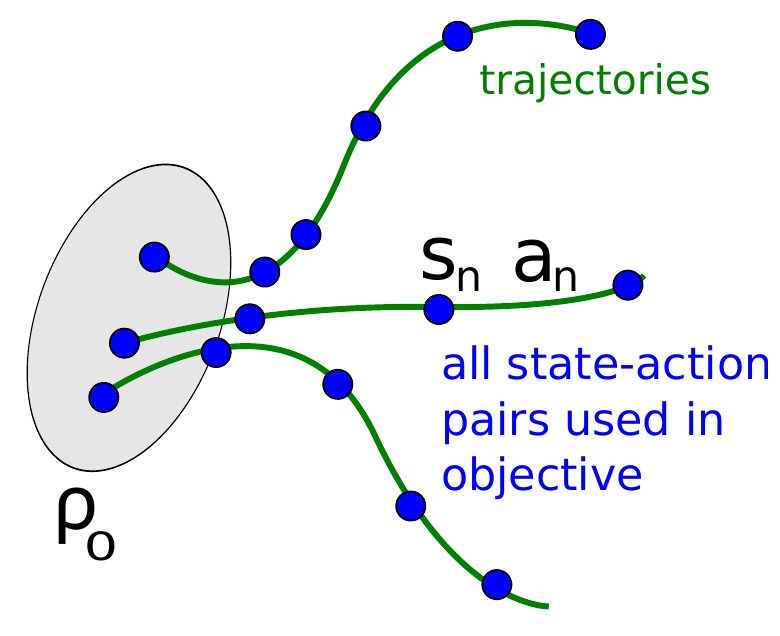
\includegraphics[height=3.2cm]{trpo_single_path.png}\par\raggedright
\begin{itemize}
  \item Roll out $\pi_{\told}$; use \textbf{every} $(s_n,a_n)$.
  \item $q=\pi_{\told}$; $\hat Q$ = discounted return-to-go.
  \item \textbf{No state resets} --- works on real systems.
\end{itemize}
\end{warmbox}
\begin{coolbox}[title={Vine}]
\centering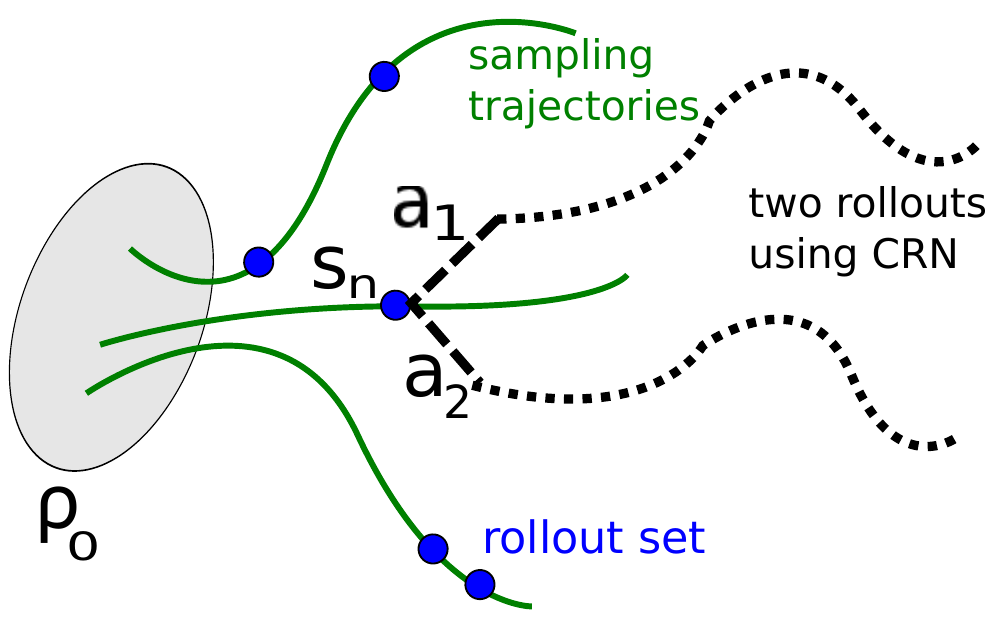
\includegraphics[height=3.2cm]{trpo_vine.png}\par\raggedright
\begin{itemize}
  \item From each $s_n$ in a \textbf{rollout set}: try $K$ actions $a_k\sim q$, a short rollout each, with common random numbers.
  \item \textbf{Lower-variance} $\hat Q$.
  \item Needs \textbf{resets} --- but only to states reached from $\rho_0$: \textbf{not} CPI's $\mu$.
\end{itemize}
\end{coolbox}
\end{pair}

{\small $q=\pi_{\theta_i}$ for continuous control, uniform for Atari (``can sometimes achieve better exploration'' --- over actions, at states already visited). Vine with continuous actions uses self-normalized IS, which removes the need for a baseline. Figures: TRPO Fig.~1.}

\subsection{4. Linear objective, quadratic constraint: the search direction}
\trpostep{4}

Approximate around $\told$:
\begin{gather*}
  L(\theta) \approx L(\told) + g^\top(\theta - \told), \qquad
  \bar D_{\mathrm{KL}}(\told,\theta) \approx \tfrac12(\theta-\told)^\top A\,(\theta-\told)
\end{gather*}

\begin{enumerate}
  \item $A_{ij}=\frac{\partial^2}{\partial\theta_i\partial\theta_j}\bar D_{\mathrm{KL}}(\told,\theta)$: the \textbf{curvature of the KL} --- the \textbf{Fisher information matrix}. Computed analytically, not from sampled score functions.
  \item The KL has \textbf{no linear term}: it is minimized (zero) at $\theta=\told$, so its gradient vanishes there.
  \item Solution direction $s\propto A^{-1}g$: the \textbf{natural gradient} --- steepest ascent when distance is measured in KL, not in $\|\theta\|$.
\end{enumerate}

\simp{$L$ and the KL are nonlinear in $\theta$; an exact constrained solve per batch is too expensive.}
     {First/second-order Taylor models $\Rightarrow$ a closed-form direction $A^{-1}g$.}
     {Valid only locally --- the step must be checked (next).}

{\small With $A^{-1}g$ and a \emph{fixed} step size we would get Kakade's (2002) natural policy gradient; TRPO enforces the constraint at each step instead (App.~\ref{app:trpo-conn}).}

\subsection{5. Computing the step: conjugate gradient + line search}
\trpostep{5}

\begin{minipage}[c]{0.54\linewidth}
\begin{enumerate}
  \item \textbf{Direction:} solve $A\,s=g$ by \textbf{conjugate gradient}. It needs only products $y\mapsto Ay$ (autodiff), $k=10$ iterations. $A$ has $|\theta|^2$ entries and is never formed.
  \item \textbf{Largest step to the KL boundary} of the quadratic model:
  \begin{gather*}
    \tfrac12(\beta s)^\top A(\beta s)=\delta \;\Rightarrow\; \beta=\sqrt{2\delta/s^\top A s}
  \end{gather*}
  \item \textbf{Backtrack} $\beta,\ \beta/2,\ \beta/4,\dots$ until
  \begin{gather*}
    L_{\told}(\theta)\ \text{improves} \ \ \text{and}\ \ \bar D_{\mathrm{KL}}(\told,\theta)\le\delta.
  \end{gather*}
\end{enumerate}
\end{minipage}\hfill
\begin{minipage}[c]{0.42\linewidth}
\centering
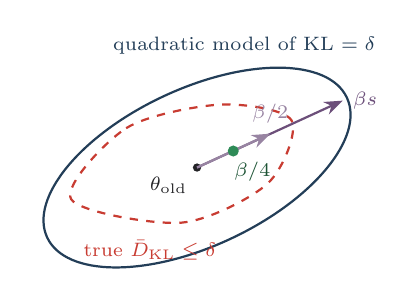
\begin{tikzpicture}[>=Stealth, font=\scriptsize]
  \draw[AtlasCool, thick, rotate=25] (0,0) ellipse (2.1 and 1.0);
  \draw[BadRed, thick, dashed] plot[smooth cycle] coordinates {(-1.6,-0.4)(-0.9,0.5)(0.3,0.8)(1.2,0.6)(0.9,-0.2)(-0.2,-0.7)};
  \fill[AtlasInk] (0,0) circle (1.5pt) node[below left] {$\told$};
  \draw[->, thick, AtlasSlate] (0,0) -- (1.85,0.85) node[right] {$\beta s$};
  \draw[->, thick, AtlasSlate!70] (0,0) -- (0.93,0.43) node[above] {$\beta/2$};
  \fill[GoodGreen] (0.46,0.21) circle (2pt);
  \node[GoodGreen!60!black] at (0.75,-0.05) {$\beta/4$ \cmark};
  \node[AtlasCool] at (0.6,1.55) {quadratic model of KL $=\delta$};
  \node[BadRed] at (-0.6,-1.05) {true $\bar D_{\mathrm{KL}}\le\delta$};
\end{tikzpicture}\\
{\scriptsize Illustrative: the full step and $\beta/2$ fail the true checks, $\beta/4$ passes.}
\end{minipage}

\simp{$A$ cannot even be stored for a neural net; the quadratic model is only local.}
     {CG with Fisher-vector products; a full step to $\delta$; a line search on the true $L$ and KL.}
     {Second order and \textbf{one step per batch} --- PPO's starting point.}

\begin{notebox}
\textbf{Fisher-vector products.} If the network outputs distribution parameters $\mu_\theta(x)$, then $A=J^\top MJ$ with $J=\partial\mu/\partial\theta$ and $M$ the analytic Fisher matrix of the distribution w.r.t.\ $\mu$. $Jy$ and $J^\top v$ are a forward-mode and a backprop pass. FVPs on $\sim$10\% of the data, so one update costs about one gradient. Without the line search, the paper reports occasional large steps with catastrophic drops.
\end{notebox}

% ---------------------------------------------------------------------------
\section{The TRPO algorithm}
% ---------------------------------------------------------------------------

\begin{algbox}{TRPO (one iteration)}
\begin{enumerate}
  \item Collect $(s,a)$ pairs with Monte Carlo $\hat Q$ estimates (single path or vine).
  \item Build the sample estimates of the surrogate $L$ and the mean-KL constraint.
  \item Compute $g=\nabla_\theta L$; solve $As=g$ with conjugate gradient (Fisher-vector products).
  \item Step size $\beta=\sqrt{2\delta/s^\top As}$; backtracking line search on $L$ and the KL.
  \item $\told\leftarrow\told+\beta s$.
\end{enumerate}
Cost per update: only slightly more than computing the gradient itself.
\end{algbox}

\subsection{Recap: from theory to practice}

\begin{center}
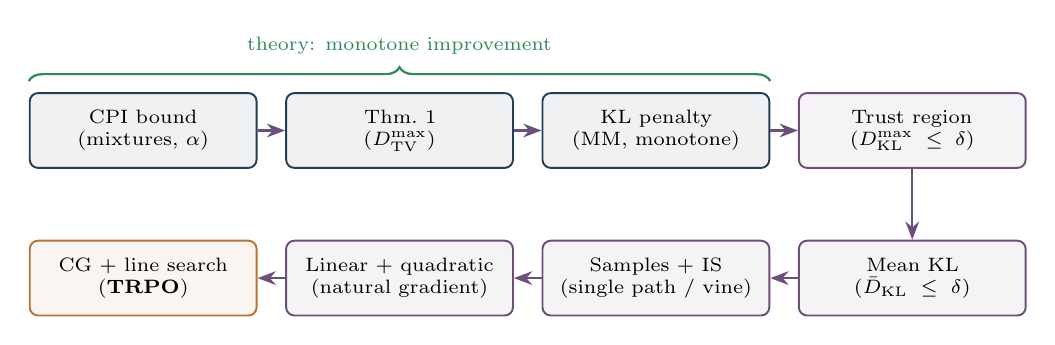
\begin{tikzpicture}[>=Stealth, node distance=0.35cm,
    box/.style={fl, cbox=AtlasCool, font=\scriptsize, minimum height=0.95cm, text width=2.6cm}]
  \node[box] (a) {CPI bound\\(mixtures, $\alpha$)};
  \node[box, right=of a] (b) {Thm.~1\\($\DTV^{\max}$)};
  \node[box, right=of b] (c) {KL penalty\\(MM, monotone)};
  \node[box, right=of c, cbox=AtlasSlate] (d) {Trust region\\($\DKL^{\max}\le\delta$)};
  \node[box, below=0.9cm of d, cbox=AtlasSlate] (e) {Mean KL\\($\bar D_{\mathrm{KL}}\le\delta$)};
  \node[box, left=of e, cbox=AtlasSlate] (f) {Samples + IS\\(single path / vine)};
  \node[box, left=of f, cbox=AtlasSlate] (g) {Linear + quadratic\\(natural gradient)};
  \node[box, left=of g, cbox=AtlasWarm] (h) {CG + line search\\(\textbf{TRPO})};
  \foreach \x/\y in {a/b, b/c, c/d, d/e, e/f, f/g, g/h} \draw[->, thick, AtlasSlate] (\x) -- (\y);
  \draw[decorate, decoration={brace, amplitude=5pt}, GoodGreen, thick] ([yshift=4pt]a.north west) -- node[above=6pt, font=\scriptsize]{theory: monotone improvement} ([yshift=4pt]c.north east);
\end{tikzpicture}
\end{center}

\begin{itemize}
  \item First three boxes: \textbf{theory}. From the trust region on: \textbf{practice} --- each arrow trades a guarantee for practicality.
  \item The theory ignores advantage-estimation error (K\&L handle it; TRPO omits it for simplicity).
  \item What is left: noisy $\hat Q$ (\textbf{GAE}) and a heavy second-order solver (\textbf{PPO}).
\end{itemize}

% ---------------------------------------------------------------------------
\section{What TRPO does not fix: where the data come from}
\label{sec:trpo-noexplore}
% ---------------------------------------------------------------------------

\begin{center}
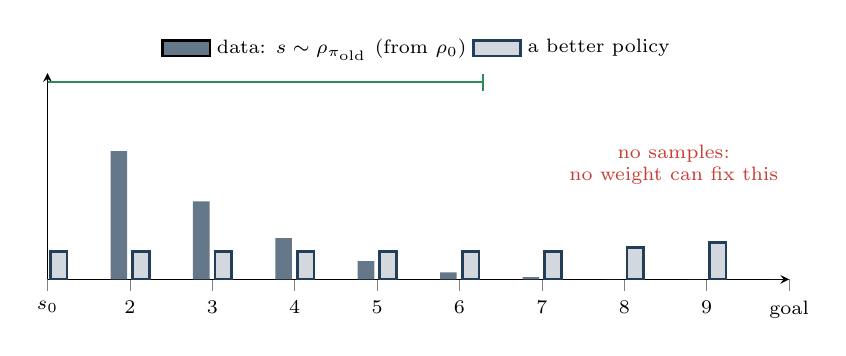
\begin{tikzpicture}
\begin{axis}[notes, width=11cm, height=4.2cm, ybar, bar width=6pt, ymin=0, ymax=0.45,
    xtick={1,...,10}, xticklabels={$s_0$,2,3,4,5,6,7,8,9,goal}, ytick=\empty,
    legend style={at={(0.5,1.02)}, anchor=south, legend columns=2}, area legend]
  \addplot[fill=AtlasCool!70, draw=none] coordinates {(1,0.4)(2,0.28)(3,0.17)(4,0.09)(5,0.04)(6,0.015)(7,0.005)(8,0)(9,0)(10,0)};
  \addlegendentry{data: $s\sim\rho_{\piold}$ (from $\rho_0$)}
  \addplot[fill=AtlasAccent!20, draw=AtlasAccent] coordinates {(1,0.06)(2,0.06)(3,0.06)(4,0.06)(5,0.06)(6,0.06)(7,0.06)(8,0.07)(9,0.08)(10,0.37)};
  \addlegendentry{a better policy}
  \draw[GoodGreen, thick, |-|] (axis cs:0.7,0.43) -- node[above, font=\scriptsize]{trust region acts here} (axis cs:6.3,0.43);
  \node[font=\scriptsize, BadRed, align=center] at (axis cs:8.6,0.25) {no samples:\\no weight can fix this};
\end{axis}
\end{tikzpicture}
\end{center}

\begin{enumerate}
  \item \textbf{Data:} $s_0\sim\rho_0$, then $\piold$ --- CPI's $\mu$ is gone.
  \item \textbf{Trust region:} limits how much $\pi$ changes \textbf{on the states we have}.
  \item \textbf{Importance sampling:} reweights \textbf{actions}, never states.
  \item \textbf{Vine:} resets only to states already reached from $\rho_0$.
\end{enumerate}

\begin{warnbox}[title={Trust region $\neq$ exploration}]
Lane B (CPI's Gap 2, \S\ref{sec:gap2-ex1}) stays open in TRPO, GAE and PPO. The only exploration left is in the actions: a stochastic policy, a uniform $q$ for the vine on Atari, and later PPO's entropy bonus.
\end{warnbox}

{\small Why TRPO still works in the experiments: $\rho_0$ and a stochastic policy already cover the relevant states (locomotion from a standing pose, Atari from the start screen).}

% ---------------------------------------------------------------------------
\section{Results}
\label{sec:trpo-results}
% ---------------------------------------------------------------------------

\subsection{Simulated robots (MuJoCo)}

\begin{minipage}[c]{0.52\linewidth}
\centering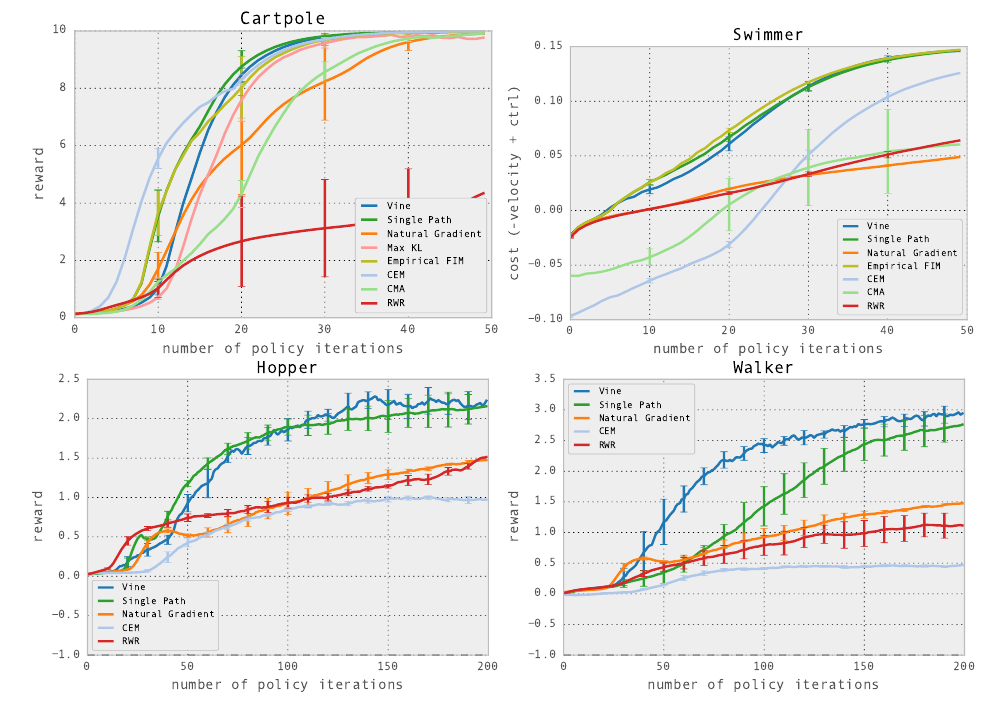
\includegraphics[width=\linewidth]{trpo_fig4_mujoco.png}\\
{\scriptsize TRPO Fig.~4: learning curves, five runs.}
\end{minipage}\hfill
\begin{minipage}[c]{0.45\linewidth}
\begin{itemize}
  \item Swimmer, hopper, walker: torques from joint states; neural-net policies.
  \item {\color{AtlasCool}\textbf{Vine, single path}}: solve all tasks, best scores.
  \item \textbf{Natural gradient} (fixed step): no hopping or walking gait.
  \item \textbf{CEM, CMA} (derivative-free): poor on the larger networks.
  \item \textbf{Max KL} (cart-pole only): a bit slower than mean KL --- simplification 2 costs little.
  \item Same $\delta=0.01$ in every experiment.
\end{itemize}
\end{minipage}

\subsection{Atari from raw pixels}

\begin{center}
\footnotesize
\setlength{\tabcolsep}{5pt}
\begin{tabular}{l r r r r r r r}
\toprule
 & B.\,Rider & Breakout & Enduro & Pong & Q*bert & Seaquest & S.\,Invaders \\
\midrule
{\color{NoteGray}Random} & {\color{NoteGray}354} & {\color{NoteGray}1.2} & {\color{NoteGray}0} & {\color{NoteGray}$-20.4$} & {\color{NoteGray}157} & {\color{NoteGray}110} & {\color{NoteGray}179} \\
{\color{NoteGray}Human} & {\color{NoteGray}7456} & {\color{NoteGray}31.0} & {\color{NoteGray}368} & {\color{NoteGray}$-3.0$} & {\color{NoteGray}18900} & {\color{NoteGray}28010} & {\color{NoteGray}3690} \\
Deep Q-learning & 4092 & 168.0 & 470 & 20.0 & 1952 & 1705 & 581 \\
UCC-I (MCTS) & 5702 & 380 & 741 & 21 & 20025 & 2995 & 692 \\
\midrule
{\color{AtlasCool}\textbf{TRPO single path}} & 1425.2 & 10.8 & \textbf{534.6} & \textbf{20.9} & \textbf{1973.5} & \textbf{1908.6} & 568.4 \\
{\color{AtlasCool}\textbf{TRPO vine}} & 859.5 & 34.2 & 430.8 & \textbf{20.9} & \textbf{7732.5} & 788.4 & 450.2 \\
\bottomrule
\end{tabular}\\[2pt]
{\scriptsize\color{NoteGray}TRPO Table~1. Bold: TRPO above Deep Q-learning. One run per game.}
\end{center}

\begin{keybox}
Not built for games --- yet the \textbf{same} algorithm and settings as for the robots give reasonable scores everywhere. (CNN policy with 33{,}500 parameters; 500 iterations $\approx$ 30 hours on 16 cores.)
\end{keybox}

% ===========================================================================
%  PART III --- GENERALIZED ADVANTAGE ESTIMATION (Schulman et al., 2015)
% ===========================================================================
\clearpage
\part{Generalized Advantage Estimation}

\partintro{\textbf{The question of Part III:} TRPO multiplies each ratio by an advantage estimate $\hat A_t$, and Monte Carlo returns make it very noisy. GAE uses a learned \textbf{value function} (the critic) and one knob $\lambda$ to trade \textbf{bias for variance} --- TD($\lambda$), applied to advantages.}

% ---------------------------------------------------------------------------
\section{Where TRPO leaves us}
% ---------------------------------------------------------------------------

\begin{center}
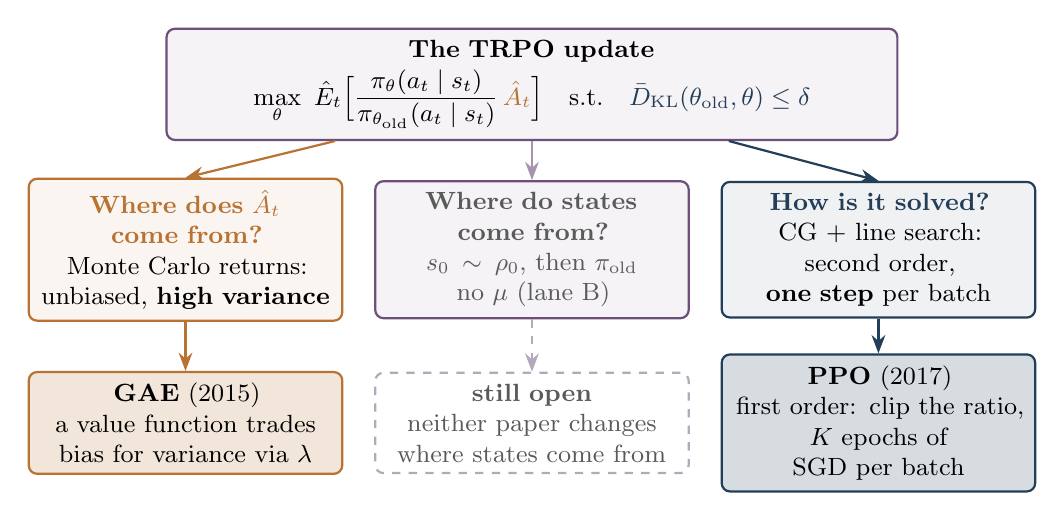
\begin{tikzpicture}[font=\small, >=Stealth,
    q/.style={fl, line width=0.8pt, text width=3.7cm, minimum height=1.05cm}]
  \node[q, cbox=AtlasSlate, text width=9cm] (trpo) at (0,0)
    {\textbf{The TRPO update}\\[2pt]
     $\displaystyle\max_\theta\ \hat\E_t\Big[\frac{\pi_\theta(a_t\mid s_t)}{\pi_{\told}(a_t\mid s_t)}\,{\color{AtlasWarm}\hat A_t}\Big]
       \quad\text{s.t.}\quad {\color{AtlasCool}\bar D_{\mathrm{KL}}(\told,\theta)\le\delta}$};
  \node[q, cbox=AtlasWarm] (adv) at (-4.4,-2.1) {\textbf{\color{AtlasWarm}Where does $\hat A_t$ come from?}\\ Monte Carlo returns:\\ unbiased, \textbf{high variance}};
  \node[q, cbox=AtlasSlate, text=NoteGray] (st) at (0,-2.1) {\textbf{Where do states come from?}\\ $s_0\sim\rho_0$, then $\piold$\\ no $\mu$ (lane B)};
  \node[q, cbox=AtlasCool] (sol) at (4.4,-2.1) {\textbf{\color{AtlasCool}How is it solved?}\\ CG + line search: second order,\\ \textbf{one step} per batch};
  \node[q, cbox=AtlasWarm, fill=AtlasWarm!18] (gae) at (-4.4,-4.3) {\textbf{GAE} (2015)\\ a value function trades\\ bias for variance via $\lambda$};
  \node[q, draw=AtlasSlate!50, dashed, text=NoteGray] (open) at (0,-4.3) {\textbf{still open}\\ neither paper changes\\ where states come from};
  \node[q, cbox=AtlasCool, fill=AtlasCool!18] (ppo) at (4.4,-4.3) {\textbf{PPO} (2017)\\ first order: clip the ratio,\\ $K$ epochs of SGD per batch};
  \draw[->, thick, AtlasWarm] (trpo.south) ++(-2.5,0) -- (adv.north);
  \draw[->, thick, AtlasSlate!60] (trpo.south) -- (st.north);
  \draw[->, thick, AtlasCool] (trpo.south) ++(2.5,0) -- (sol.north);
  \draw[->, thick, AtlasWarm] (adv) -- (gae);
  \draw[->, thick, AtlasSlate!50, dashed] (st) -- (open);
  \draw[->, thick, AtlasCool] (sol) -- (ppo);
\end{tikzpicture}
\end{center}

{\small The update is written as in the GAE paper (Sec.~6.1, Eq.~31). TRPO itself used Monte Carlo $\hat Q$, which differs from an advantage only by a baseline. PPO's intro lists TRPO's other drawbacks: complicated, and incompatible with noise (dropout) or parameter sharing between policy and value.}

% ---------------------------------------------------------------------------
\section{Setting}
% ---------------------------------------------------------------------------

\paper{High-Dimensional Continuous Control Using Generalized Advantage Estimation}
  {Schulman, Moritz, Levine, Jordan \& Abbeel}{ICLR 2016 (arXiv 2015)}
  {GAE$(\gamma,\lambda)$ --- TD($\lambda$) for advantages, plus a trust-region value fit}
  {gae.md}

\begin{enumerate}
  \item Same MDP as TRPO: start distribution $\rho_0$, unknown dynamics, reward $r_t=r(s_t,a_t,s_{t+1})$.
  \item \textbf{Undiscounted} goal: maximize $\E\big[\sum_t r_t\big]$ (assumed finite).
  \item $\gamma$ is \textbf{not part of the problem}: it is an algorithm knob that trades bias for variance.
  \item Any policy-gradient method --- here TRPO for the policy, and a trust region for $V_\phi$ too.
  \item 3D robots, neural nets with $>10^4$ parameters, torques from raw kinematics.
\end{enumerate}

\begin{notebox}
All quantities are unnormalized, like TRPO and unlike CPI. The formula itself appeared earlier (Kimura \& Kobayashi 1998; Wawrzy\'nski 2009); the paper's contribution is the analysis that makes it usable with batch trust-region methods, plus the trust-region value fit.
\end{notebox}

\subsection{What GAE fixes --- and what it does not}

\begin{minipage}[c]{0.5\linewidth}
\centering
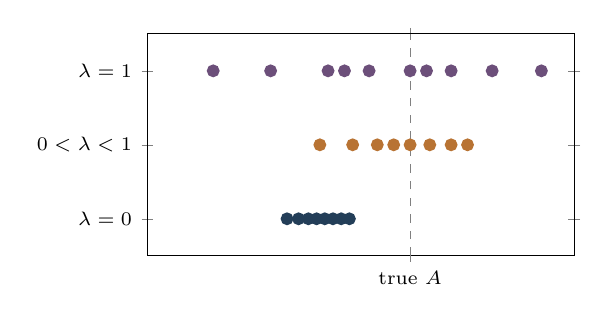
\begin{tikzpicture}
\begin{axis}[notes, width=7cm, height=4.4cm, xmin=-1.3, xmax=1.3, ymin=-0.5, ymax=2.5,
    ytick={0,1,2}, yticklabels={$\lambda=0$, $0<\lambda<1$, $\lambda=1$}, xtick={0.3}, xticklabels={true $A$},
    axis lines=box, only marks, mark size=1.8pt]
  \addplot[AtlasSlate, mark=*] coordinates {(-0.9,2)(-0.55,2)(-0.2,2)(0.05,2)(0.3,2)(0.55,2)(0.8,2)(1.1,2)(0.4,2)(-0.1,2)};
  \addplot[AtlasWarm, mark=*] coordinates {(-0.25,1)(-0.05,1)(0.1,1)(0.2,1)(0.3,1)(0.42,1)(0.55,1)(0.65,1)};
  \addplot[AtlasCool, mark=*] coordinates {(-0.45,0)(-0.38,0)(-0.32,0)(-0.27,0)(-0.22,0)(-0.17,0)(-0.12,0)(-0.07,0)};
  \draw[dashed, gray] (axis cs:0.3,-0.5) -- (axis cs:0.3,2.5);
\end{axis}
\end{tikzpicture}\\
{\scriptsize Each dot: one estimate $\hat A_t$ of the same $(s_t,a_t)$ (schematic).}
\end{minipage}\hfill
\begin{minipage}[c]{0.47\linewidth}
\begin{enumerate}
  \item TRPO multiplies each ratio by $\hat A_t$. From one rollout: \textbf{unbiased}, but \textbf{very noisy} (top row).
  \item A learned \textbf{value function} $V$ --- the \emph{critic}: low noise, but \textbf{biased} if $V$ is wrong (bottom row).
  \item $\lambda$ slides between the two: a \textbf{bias--variance knob} (middle row).
\end{enumerate}
\end{minipage}

\begin{pair}
\begin{keybox}[title={Fixes}]
Noisy update directions $\Rightarrow$ fewer samples per step.
\end{keybox}
\begin{warnbox}[title={Not an exploration knob}]
$\lambda$ changes how we \emph{score} sampled actions, not \emph{which states} we visit.
\end{warnbox}
\end{pair}

\begin{notebox}
GAE abstract: two challenges --- ``the large number of samples typically required, and the difficulty of obtaining stable and steady improvement''. Value functions attack the first, a trust region for both policy and value attacks the second. Sec.~1: ``bias is more pernicious --- even with an unlimited number of samples, bias can cause the algorithm to fail to converge.''
\end{notebox}

% ---------------------------------------------------------------------------
\section{Which weight multiplies the score function?}
% ---------------------------------------------------------------------------

All policy-gradient estimators have the same form:
\begin{gather*}
  g = \E\Big[\sum_{t\ge0} \Psi_t\,\nabla_\theta\log\pi_\theta(a_t\mid s_t)\Big]
\end{gather*}

\begin{minipage}[c]{0.5\linewidth}
Same expectation for each choice of $\Psi_t$ --- \textbf{different variance}:\par\vspace{2pt}
\small
\begin{tabular}{r l l}
\toprule
 & $\Psi_t$ & \\
\midrule
1 & $\sum_{t'\ge0} r_{t'}$ & total return \\
2 & $\sum_{t'\ge t} r_{t'}$ & reward after $a_t$ \\
3 & $\sum_{t'\ge t} r_{t'} - b(s_t)$ & with a baseline \\
4 & $Q^\pi(s_t,a_t)$ & action value \\
5 & {\color{AtlasCool}$\boldsymbol{A^\pi(s_t,a_t)}$} & {\color{AtlasCool}\textbf{advantage}} \\
6 & $r_t + V^\pi(s_{t+1}) - V^\pi(s_t)$ & TD residual \\
\bottomrule
\end{tabular}
\end{minipage}\hfill
\begin{minipage}[c]{0.46\linewidth}
\begin{keybox}[title={Why the advantage}]
\begin{itemize}
  \item ``Almost the lowest possible variance'' (Greensmith et al., 2004).
  \item A step along $A\,\nabla\log\pi$ raises $\pi(a\mid s)$ \textbf{iff} $a$ beats the average $V^\pi$ --- the gaps of the Notation figure in Part~I.
\end{itemize}
\end{keybox}
\end{minipage}

\begin{slatebox}[title={The discount as a knob}]
The discounted gradient $g^\gamma$ uses $A^{\pi,\gamma}$, which ignores effects $\gg\frac{1}{1-\gamma}$ steps later $\Rightarrow$ less variance, \textbf{some bias}. An estimator $\hat A_t$ is \emph{$\gamma$-just} if it gives an unbiased estimate of $g^\gamma$ (Def.~1, Prop.~1). From here on, bias means bias \emph{relative to} $g^\gamma$.
\end{slatebox}

% ---------------------------------------------------------------------------
\section{GAE: TD($\lambda$) for advantages}
% ---------------------------------------------------------------------------

Four steps, from one TD residual to all of them.

\begin{enumerate}
  \item \textbf{TD residual} --- one reward, then $V$:
  \begin{gather*}
    \delta_t^V = r_t + \gamma V(s_{t+1}) - V(s_t)
  \end{gather*}
  \item \textbf{$k$ residuals} --- $\hat A_t^{(k)}=\sum_{l<k}\gamma^l\delta_{t+l}^V$ telescopes to
  \begin{gather*}
    \hat A_t^{(k)} = -V(s_t) + \textstyle\sum_{l=0}^{k-1}\gamma^l r_{t+l} + \gamma^k V(s_{t+k})
  \end{gather*}
  \item \textbf{All of them} --- the return minus a baseline:
  \begin{gather*}
    \hat A_t^{(\infty)} = \textstyle\sum_{l\ge0}\gamma^l r_{t+l} - V(s_t)
  \end{gather*}
  \item \textbf{GAE} --- average all $k$ with weights $(1-\lambda)\lambda^{k-1}$:
\end{enumerate}

\begin{eqbox}
\begin{gather*}
  \hat A_t^{\mathrm{GAE}(\gamma,\lambda)} = (1-\lambda)\textstyle\sum_{k\ge1}\lambda^{k-1}\hat A_t^{(k)} = \textstyle\sum_{l\ge0}(\gamma\lambda)^l\,\delta_{t+l}^V
\end{gather*}
\end{eqbox}

\begin{minipage}[c]{0.5\linewidth}
\centering
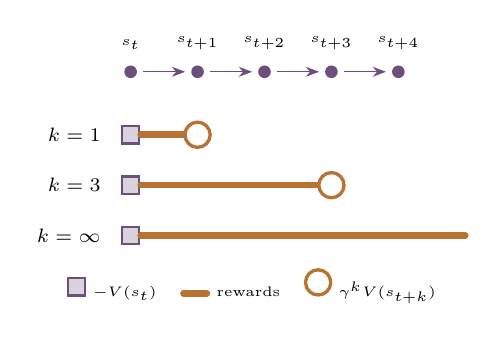
\begin{tikzpicture}[x=0.85cm, y=0.8cm, >=Stealth,
    st/.style={circle, fill=AtlasSlate, minimum size=0.16cm, inner sep=0pt},
    real/.style={AtlasWarm, line width=2.4pt, line cap=round},
    boot/.style={circle, draw=AtlasWarm, very thick, fill=white, minimum size=0.32cm, inner sep=0pt},
    base/.style={rectangle, draw=AtlasSlate, thick, fill=AtlasSlate!25, minimum size=0.22cm, inner sep=0pt},
    lab/.style={font=\scriptsize, anchor=east}]
  \foreach \i/\n in {0/t, 1/t{+}1, 2/t{+}2, 3/t{+}3, 4/t{+}4} {
    \node[st] (s\i) at (\i,0) {};
    \node[font=\tiny, above=2pt of s\i] {$s_{\n}$};}
  \foreach \i/\j in {0/1, 1/2, 2/3, 3/4} \draw[->, AtlasSlate, shorten <=2pt, shorten >=2pt] (s\i) -- (s\j);
  \node[lab] at (-0.3,-1.0) {$k=1$};
  \node[base] at (0,-1.0) {}; \draw[real] (0.15,-1.0) -- (1,-1.0); \node[boot] at (1,-1.0) {};
  \node[lab] at (-0.3,-1.8) {$k=3$};
  \node[base] at (0,-1.8) {}; \draw[real] (0.15,-1.8) -- (3,-1.8); \node[boot] at (3,-1.8) {};
  \node[lab] at (-0.3,-2.6) {$k=\infty$};
  \node[base] at (0,-2.6) {}; \draw[real] (0.15,-2.6) -- (5.0,-2.6);
  \node[font=\tiny, anchor=west] at (-1.1,-3.4)
    {\tikz\node[base]{}; $-V(s_t)$ \;\; \tikz\draw[real] (0,0) -- (0.35,0); rewards \;\; \tikz\node[boot] {}; $\gamma^kV(s_{t+k})$};
\end{tikzpicture}
\end{minipage}\hfill
\begin{minipage}[c]{0.47\linewidth}
\centering
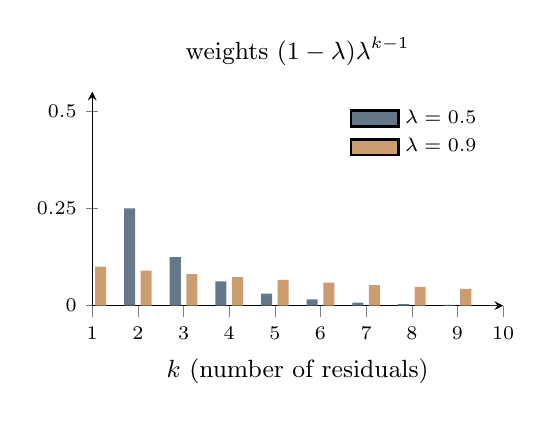
\begin{tikzpicture}
\begin{axis}[notes, width=6.8cm, height=4.3cm, ybar, bar width=4pt, ymin=0, ymax=0.55,
    xlabel={$k$ (number of residuals)}, xtick={1,...,10}, ytick={0,0.25,0.5},
    legend pos=north east, area legend, title={\small weights $(1-\lambda)\lambda^{k-1}$}]
  \addplot[fill=AtlasCool!70, draw=none] coordinates {(1,0.5)(2,0.25)(3,0.125)(4,0.0625)(5,0.031)(6,0.016)(7,0.008)(8,0.004)(9,0.002)(10,0.001)};
  \addlegendentry{$\lambda=0.5$}
  \addplot[fill=AtlasWarm!70, draw=none] coordinates {(1,0.1)(2,0.09)(3,0.081)(4,0.073)(5,0.066)(6,0.059)(7,0.053)(8,0.048)(9,0.043)(10,0.039)};
  \addlegendentry{$\lambda=0.9$}
\end{axis}
\end{tikzpicture}
\end{minipage}

\begin{center}
\small
\begin{tabular}{l l l}
\toprule
 & $\lambda=0$: \ $\hat A_t=\delta_t^V$ & $\lambda=1$: \ $\hat A_t=\sum_l\gamma^lr_{t+l}-V(s_t)$ \\
\midrule
bias & biased unless $V=V^{\pi,\gamma}$ & unbiased for $g^\gamma$, \textbf{any} $V$ \\
variance & low & high \\
\bottomrule
\end{tabular}
\end{center}

\begin{notebox}
The same picture as TD(0)$\to$Monte Carlo in Part~I: TD($\lambda$) estimates a value, GAE an advantage; the only change is the baseline $-V(s_t)$ at the start of every row. The bias shrinks with $k$ because the bootstrapped term $\gamma^kV(s_{t+k})$ is discounted more, while $-V(s_t)$ never adds bias (it is a baseline).
\end{notebox}

% ---------------------------------------------------------------------------
\section{Two knobs, two kinds of bias}
% ---------------------------------------------------------------------------

\begin{minipage}[c]{0.5\linewidth}
\centering
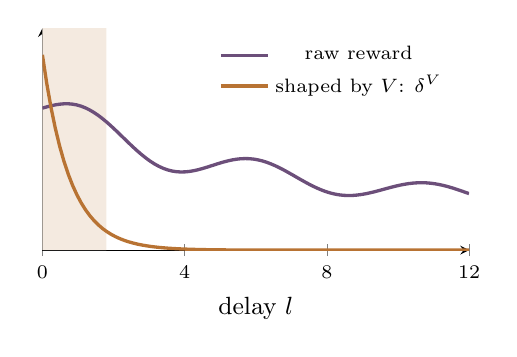
\begin{tikzpicture}
\begin{axis}[notes, width=7cm, height=4.4cm, xmin=0, xmax=12, ymin=0, ymax=1.25,
    xlabel={delay $l$}, ytick=\empty, xtick={0,4,8,12}, legend pos=north east,
    declare function={raw(\x) = 0.25 + 0.55*exp(-0.18*\x) + 0.12*sin(deg(1.3*\x))*exp(-0.08*\x);
                       shaped(\x) = 1.1*exp(-1.3*\x);}]
  \addplot[draw=none, fill=AtlasWarm!15, forget plot] coordinates {(0,0)(0,1.25)(1.8,1.25)(1.8,0)} \closedcycle;
  \addplot[AtlasSlate, very thick, domain=0:12, samples=100] {raw(x)};
  \addlegendentry{raw reward}
  \addplot[AtlasWarm, very thick, domain=0:12, samples=100] {shaped(x)};
  \addlegendentry{shaped by $V$: $\delta^V$}
\end{axis}
\end{tikzpicture}\\
{\scriptsize $\chi(l;s,a)=\E[r_{t+l}\mid s,a]-\E[r_{t+l}\mid s]$: how long $a_t$ keeps mattering.}
\end{minipage}\hfill
\begin{minipage}[c]{0.47\linewidth}
\begin{pair}[1]
\begin{slatebox}[title={$\gamma$: cut the horizon}]
\small Drops effects after $\approx\frac{1}{1-\gamma}$ steps. Biased \textbf{even with the exact} $V$.
\end{slatebox}
\begin{warmbox}[title={$\lambda$: shape, then cut again}]
\small $\delta^V$ is the reward \emph{shaped} by $\Phi=V$: a good $V$ pulls the effect of $a_t$ to $l\approx0$. Biased \textbf{only if $V$ is wrong}.
\end{warmbox}
\end{pair}
\end{minipage}

\begin{keybox}
So the best $\lambda$ is \textbf{lower} than the best $\gamma$ (numbers in \S\ref{sec:gae-results}).
\end{keybox}

\begin{notebox}
\textbf{Reward shaping} (Ng et al., 1999): $\tilde r=r+\gamma\Phi(s')-\Phi(s)$ leaves $A^{\pi,\gamma}$ unchanged. With $\Phi=V$ it is exactly $\delta^V$, and GAE is the $(\gamma\lambda)$-discounted sum of shaped rewards (Eq.~20). With $\Phi=V^{\pi,\gamma}$ the shaped response is nonzero only at $l=0$. Response function: $A^{\pi,\gamma}(s,a)=\sum_l\gamma^l\chi(l;s,a)$ (Eq.~22). The curves are illustrative.
\end{notebox}

% ---------------------------------------------------------------------------
\section{Actor--critic: policy and value networks}
% ---------------------------------------------------------------------------

\begin{minipage}[c]{0.5\linewidth}
\centering
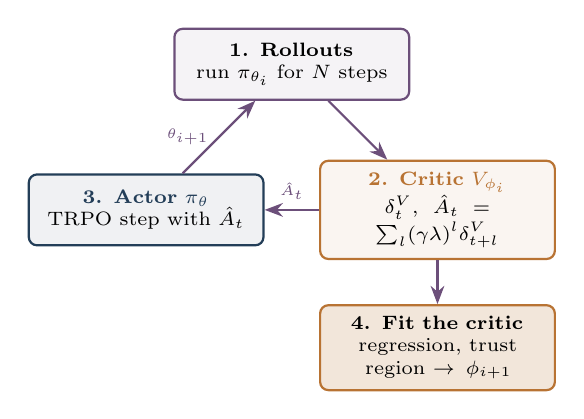
\begin{tikzpicture}[font=\scriptsize, >=Stealth,
    ac/.style={fl, line width=0.8pt, text width=2.7cm, minimum height=0.9cm, font=\scriptsize}]
  \node[ac, cbox=AtlasSlate] (env) at (0,0) {\textbf{1. Rollouts}\\ run $\pi_{\theta_i}$ for $N$ steps};
  \node[ac, cbox=AtlasWarm] (crit) at (1.85,-1.85) {\textbf{\color{AtlasWarm}2. Critic $V_{\phi_i}$}\\ $\delta_t^V$, \ $\hat A_t=\sum_l(\gamma\lambda)^l\delta_{t+l}^V$};
  \node[ac, cbox=AtlasCool] (act) at (-1.85,-1.85) {\textbf{\color{AtlasCool}3. Actor $\pi_\theta$}\\ TRPO step with $\hat A_t$};
  \node[ac, cbox=AtlasWarm, fill=AtlasWarm!18] (fit) at (1.85,-3.6) {\textbf{4. Fit the critic}\\ regression, trust region $\to\phi_{i+1}$};
  \draw[->, thick, AtlasSlate] (env) -- (crit);
  \draw[->, thick, AtlasSlate] (crit) -- node[above, font=\tiny]{$\hat A_t$} (act);
  \draw[->, thick, AtlasSlate] (crit) -- (fit);
  \draw[->, thick, AtlasSlate] (act) -- node[left, font=\tiny]{$\theta_{i+1}$} (env);
\end{tikzpicture}
\end{minipage}\hfill
\begin{minipage}[c]{0.47\linewidth}
\begin{itemize}
  \item \textbf{Actor}: the policy network, updated by TRPO.
  \item \textbf{Critic}: a second network $V_\phi(s)\approx V^{\pi,\gamma}(s)$, fitted by regression to Monte Carlo returns $\hat V_n=\sum_l\gamma^lr_{n+l}$.
  \item \textbf{Order matters}: fit $V$ \emph{after} computing $\hat A_t$ --- an overfit $V$ makes every $\delta_t^V=0$.
\end{itemize}
\end{minipage}

\begin{warmbox}[title={Value fit with a trust region}]
\begin{gather*}
  \min_\phi\ \sum_n \big\|V_\phi(s_n) - \hat V_n\big\|^2
  \quad \text{s.t.}\ \ \frac1N\sum_n \frac{\|V_\phi(s_n) - V_{\phi_{\mathrm{old}}}(s_n)\|^2}{2\sigma^2} \le \epsilon
\end{gather*}
\begin{itemize}
  \item $=$ a KL trust region for a Gaussian with mean $V_\phi(s)$; $\sigma^2$ is the current mean squared error.
  \item Solved with conjugate gradient, like TRPO.
  \item Keeps $V$ from overfitting the latest batch --- the ``stable improvement'' challenge of the abstract.
\end{itemize}
\end{warmbox}

\begin{notebox}
Unlike Q-learning-style critics (e.g.\ SAC, which learns $Q(s,a)$ off-policy), GAE's critic is a state value $V(s)$ fitted \textbf{on-policy}. Networks: three hidden layers (100, 50, 25 tanh units) for both policy and value. TD($\lambda$) targets for the critic made no difference.
\end{notebox}

% ---------------------------------------------------------------------------
\section{Results: choosing $\gamma$ and $\lambda$}
\label{sec:gae-results}
% ---------------------------------------------------------------------------

\begin{minipage}[c]{0.56\linewidth}
\centering
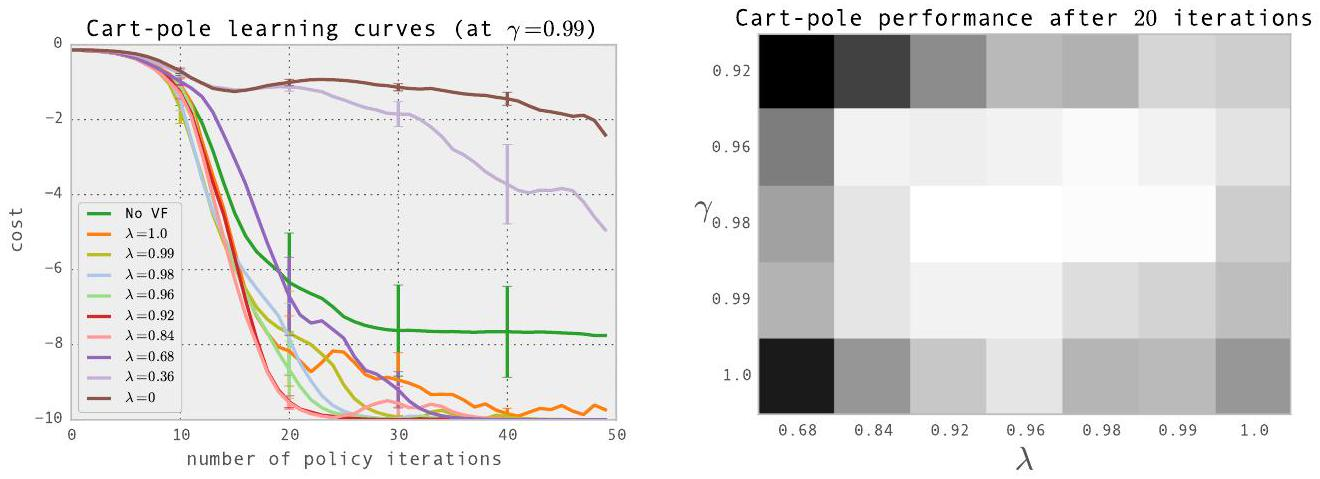
\includegraphics[width=\linewidth]{gae_fig2_sweep.jpg}\\[2pt]
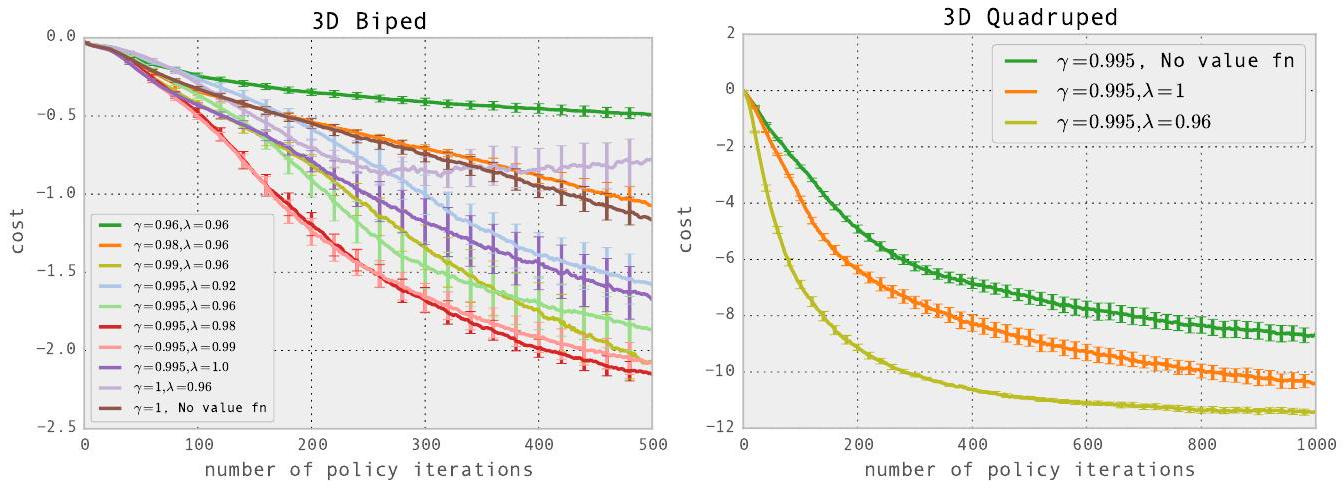
\includegraphics[width=\linewidth]{gae_fig3_3d.jpg}\\
{\scriptsize GAE Figs.~2--3. Cost $=$ negative reward (lower is better).}
\end{minipage}\hfill
\begin{minipage}[c]{0.41\linewidth}
\textbf{Cart-pole} (top)
\begin{itemize}
  \item best at intermediate $\lambda\in[0.92,0.99]$, $\gamma\in[0.96,0.99]$
  \item $\lambda=0$ and ``No VF'' (time-dependent baseline only) much worse
\end{itemize}
\textbf{3D biped, quadruped} (bottom)
\begin{itemize}
  \item best $\gamma\in[0.99,0.995]$, $\lambda\in[0.96,0.99]$
  \item the biped runs after 1000 iterations $\approx$ 5.8 days of simulated time
\end{itemize}
\end{minipage}

\begin{keybox}
Best $\lambda$ $<$ best $\gamma$: $\lambda$ adds bias only if $V$ is wrong. Discussion: $\lambda\in[0.9,0.99]$ usually best; App.~A.2: the $\lambda=0$ estimator was ``prohibitively'' biased.
\end{keybox}

% ===========================================================================
%  PART IV --- PROXIMAL POLICY OPTIMIZATION (Schulman et al., 2017)
% ===========================================================================
\clearpage
\part{Proximal Policy Optimization}

\partintro{\textbf{The question of Part IV:} TRPO's second-order step uses each batch \textbf{once}. PPO wants \textbf{many first-order SGD steps} per batch without leaving the trust region. It \textbf{clips} the importance ratio, so the objective itself stops rewarding large moves.}

% ---------------------------------------------------------------------------
\section{Setting and motivation}
% ---------------------------------------------------------------------------

\paper{Proximal Policy Optimization Algorithms}
  {Schulman, Wolski, Dhariwal, Radford \& Klimov}{arXiv 2017 (OpenAI)}
  {PPO --- TRPO's reliability with only first-order SGD}
  {proximal\_policy\_optimization\_algorithms.md}

\begin{itemize}
  \item Same setting as TRPO; advantages $\hat A_t$ from (truncated) \textbf{GAE}.
  \item \textbf{TRPO}: complicated; no dropout, no parameter sharing between policy and value.
  \item \textbf{Vanilla PG}: several steps on the same batch $\Rightarrow$ destructively large updates.
  \item \textbf{Goal}: reuse each batch for many SGD steps, without leaving the trust region.
  \item Tested on MuJoCo and 49 Atari games.
\end{itemize}

\begin{notebox}
``Vanilla'' PG estimator: $\hat g=\hat\E_t[\nabla_\theta\log\pi_\theta(a_t\mid s_t)\hat A_t]$, from the loss $L^{PG}=\hat\E_t[\log\pi_\theta\,\hat A_t]$; $\hat\E_t$ is the empirical average over a batch. Q-learning with function approximation is also dismissed: it fails on many simple problems and had no strong continuous-control results at the time.
\end{notebox}

\subsection{The goal: many SGD steps per batch}

\begin{center}
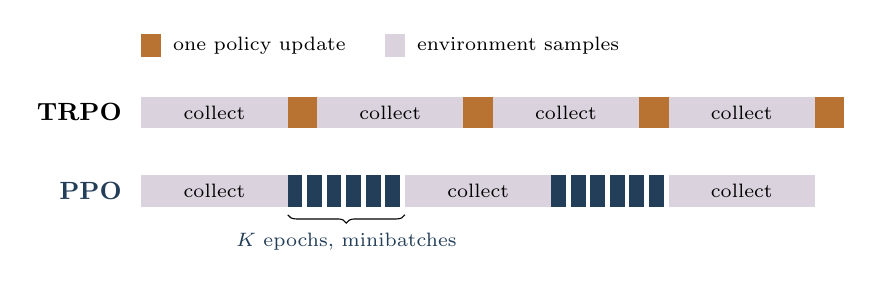
\begin{tikzpicture}[x=0.62cm, y=1cm, font=\scriptsize]
  \node[font=\small\bfseries, anchor=east] at (-0.2,1.3) {TRPO};
  \foreach \a/\b in {0/3, 3.6/6.6, 7.2/10.2, 10.8/13.8} {
    \fill[AtlasSlate!25] (\a,1.1) rectangle (\b,1.5); \node at ({(\a+\b)/2},1.3) {collect};
    \fill[AtlasWarm] (\b,1.1) rectangle (\b+0.6,1.5);}
  \node[font=\small\bfseries, anchor=east, text=AtlasCool] at (-0.2,0.3) {PPO};
  \foreach \a/\b in {0/3, 5.4/8.4, 10.8/13.8} {
    \fill[AtlasSlate!25] (\a,0.1) rectangle (\b,0.5); \node at ({(\a+\b)/2},0.3) {collect};}
  \foreach \b in {3, 8.4} {
    \foreach \k in {0,...,5} \fill[AtlasCool] (\b+\k*0.4,0.1) rectangle (\b+\k*0.4+0.3,0.5);}
  \draw[decorate, decoration={brace, amplitude=3pt, mirror}] (3,0.0) -- node[below=3pt, text=AtlasCool]{$K$ epochs, minibatches} (5.4,0.0);
  \fill[AtlasWarm] (0,2.0) rectangle (0.4,2.3); \node[anchor=west] at (0.45,2.15) {one policy update};
  \fill[AtlasSlate!25] (5,2.0) rectangle (5.4,2.3); \node[anchor=west] at (5.45,2.15) {environment samples};
\end{tikzpicture}
\end{center}

\begin{pair}
\begin{slatebox}[title={TRPO}]
\small One (expensive, carefully constrained) step, then the batch is thrown away.
\end{slatebox}
\begin{coolbox}[title={PPO}]
\small Squeeze the same batch with cheap first-order steps: $K$ epochs of minibatch SGD.
\end{coolbox}
\end{pair}

\begin{warnbox}[title={Why naive reuse fails}]
The data came from $\piold$: the surrogate is trustworthy only near $r_t=1$. For one sample with $\hat A_t>0$ the term $r_t\hat A_t$ is linear in $r_t$ --- \textbf{nothing says stop}. Unchecked, repeated steps give \textbf{destructively large} updates. Only TRPO's KL constraint stopped it; PPO asks how to stop it with an ordinary first-order optimizer.
\end{warnbox}

% ---------------------------------------------------------------------------
\section{Back to the CPI surrogate}
% ---------------------------------------------------------------------------

The ratio is TRPO's importance weight:
\begin{gather*}
  r_t(\theta) = \frac{\pi_\theta(a_t\mid s_t)}{\pi_{\told}(a_t\mid s_t)}, \qquad r_t(\told)=1.
\end{gather*}

\begin{eqbox}
\begin{gather*}
  L^{CPI}(\theta) = \hat\E_t\big[r_t(\theta)\,\hat A_t\big] \qquad \text{(``CPI'': Kakade \& Langford, where this objective was proposed)}
\end{gather*}
\end{eqbox}

{\small It is TRPO's $L_{\told}$ written with sample averages; its gradient at $\told$ is the vanilla policy gradient. Many SGD steps on $L^{CPI}$ alone: $r_t$ runs far from 1 $\Rightarrow$ huge updates. Normalized score $-0.39$: worse than random (\S\ref{sec:ppo-ablation}).}

\textbf{Three ways to stay close:}

\begin{pair}[3]
\begin{slatebox}[title={Constraint (TRPO)}]
\small s.t.\ $\hat\E_t[\DKL]\le\delta$\\[2pt]
{\scriptsize second-order solver}
\end{slatebox}
\begin{warmbox}[title={Penalty (baseline)}]
\small $-\beta\,\hat\E_t[\DKL]$\\[2pt]
{\scriptsize no single $\beta$ works $\to$ adapt it}
\end{warmbox}
\begin{coolbox}[title={Clip (``PPO'')}]
\small no gain once $|r_t-1|>\epsilon$\\[2pt]
{\scriptsize first order}
\end{coolbox}
\end{pair}

{\small The penalty form is what TRPO's theory suggests; TRPO used a constraint because ``it is hard to choose a single value of $\beta$ that performs well across different problems --- or even within a single problem''.}

% ---------------------------------------------------------------------------
\section{The clipped surrogate objective}
% ---------------------------------------------------------------------------

\begin{eqbox}
\begin{gather*}
  L^{CLIP}(\theta) = \hat\E_t\Big[\min\big(r_t(\theta)\hat A_t,\ \mathrm{clip}(r_t(\theta),1-\epsilon,1+\epsilon)\,\hat A_t\big)\Big],
  \qquad \epsilon = 0.2
\end{gather*}
\end{eqbox}

One term of the sum, as a function of the ratio $r$:

\begin{center}
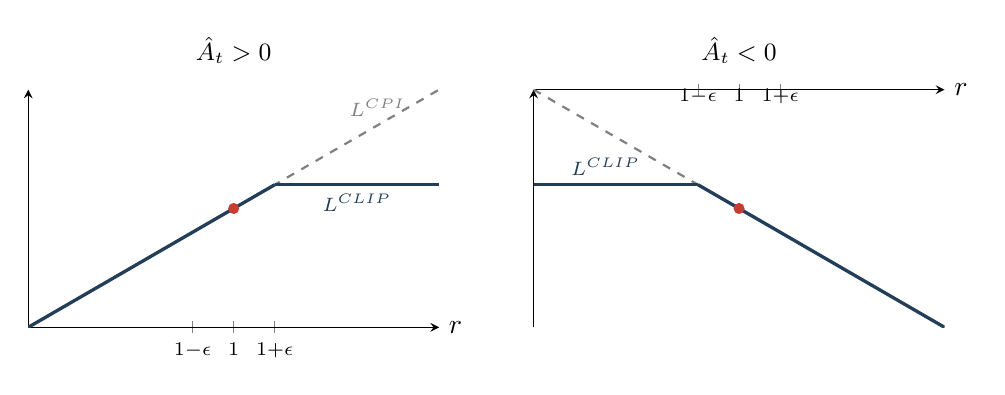
\begin{tikzpicture}
\begin{axis}[notes, name=pos, width=6.8cm, height=4.6cm, xmin=0, xmax=2, ymin=0, ymax=2,
    xlabel={$r$}, xtick={0.8,1,1.2}, xticklabels={$1{-}\epsilon$,1,$1{+}\epsilon$}, ytick=\empty,
    title={\small $\hat A_t>0$}, axis lines=middle, x label style={at={(axis description cs:1,0)}, anchor=west}]
  \addplot[gray, thick, dashed, domain=0:2] {x};
  \addplot[AtlasCool, very thick, domain=0:1.2] {x};
  \addplot[AtlasCool, very thick, domain=1.2:2] {1.2};
  \fill[BadRed] (axis cs:1,1) circle (2pt);
  \node[font=\scriptsize, gray] at (axis cs:1.7,1.85) {$L^{CPI}$};
  \node[font=\scriptsize, AtlasCool] at (axis cs:1.6,1.05) {$L^{CLIP}$};
\end{axis}
\begin{axis}[notes, at={(pos.east)}, anchor=west, xshift=1.2cm, width=6.8cm, height=4.6cm, xmin=0, xmax=2, ymin=-2, ymax=0,
    xlabel={$r$}, xtick={0.8,1,1.2}, xticklabels={$1{-}\epsilon$,1,$1{+}\epsilon$}, ytick=\empty,
    title={\small $\hat A_t<0$}, axis lines=middle, x label style={at={(axis description cs:1,1)}, anchor=west},
    xticklabel style={yshift=6pt}]
  \addplot[gray, thick, dashed, domain=0:2] {-x};
  \addplot[AtlasCool, very thick, domain=0:0.8] {-0.8};
  \addplot[AtlasCool, very thick, domain=0.8:2] {-x};
  \fill[BadRed] (axis cs:1,-1) circle (2pt);
  \node[font=\scriptsize, AtlasCool] at (axis cs:0.35,-0.65) {$L^{CLIP}$};
\end{axis}
\end{tikzpicture}\\
{\scriptsize Redrawn from PPO Fig.~1. Red dot: the start of the optimization, $r=1$. Dashed: $L^{CPI}$.}
\end{center}

\begin{pair}
\begin{coolbox}[title={$\hat A_t>0$: raise $\pi(a_t\mid s_t)$}]
\small
\begin{itemize}
  \item No extra gain past $1+\epsilon$ (flat).
  \item Wrong way ($r<1-\epsilon$): \textbf{not} clipped, still costs.
\end{itemize}
\end{coolbox}
\begin{coolbox}[title={$\hat A_t<0$: lower $\pi(a_t\mid s_t)$}]
\small
\begin{itemize}
  \item No extra gain below $1-\epsilon$ (flat).
  \item Wrong way ($r>1+\epsilon$): \textbf{not} clipped, the loss keeps growing.
\end{itemize}
\end{coolbox}
\end{pair}

\begin{keybox}[title={A pessimistic bound}]
\begin{enumerate}
  \item The $\min$ gives $L^{CLIP}\le L^{CPI}$: clipping removes \textbf{gains}, never hides \textbf{losses}.
  \item Moving the wrong way keeps its gradient: the update can always pull $r_t$ \textbf{back} toward 1.
  \item $L^{CLIP}=L^{CPI}$ to first order at $\told$.
\end{enumerate}
\end{keybox}

{\small PPO Fig.~2: along the update direction, $L^{CLIP}$ peaks at a KL of about 0.02 (Hopper).}

\subsection{What clipping replaces}

\begin{center}
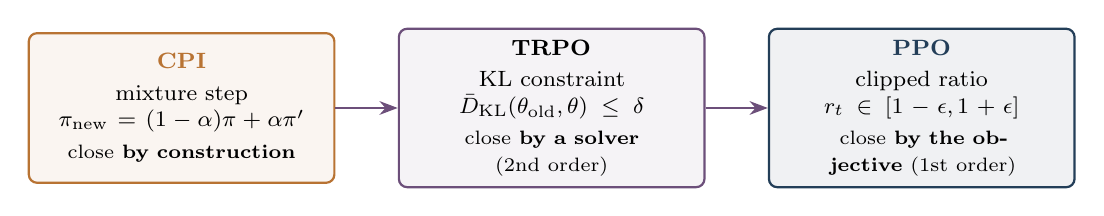
\begin{tikzpicture}[font=\footnotesize, >=Stealth,
    cr/.style={fl, line width=0.8pt, text width=3.6cm, minimum height=1.9cm, font=\footnotesize}]
  \node[cr, cbox=AtlasWarm] (c) at (0,0) {\textbf{\color{AtlasWarm}CPI}\\[2pt] mixture step\\ $\pinew=(1-\alpha)\pi+\alpha\pi'$\\[2pt] {\scriptsize close \textbf{by construction}}};
  \node[cr, cbox=AtlasSlate] (t) at (4.7,0) {\textbf{TRPO}\\[2pt] KL constraint\\ $\bar D_{\mathrm{KL}}(\told,\theta)\le\delta$\\[2pt] {\scriptsize close \textbf{by a solver} (2nd order)}};
  \node[cr, cbox=AtlasCool] (p) at (9.4,0) {\textbf{\color{AtlasCool}PPO}\\[2pt] clipped ratio\\ $r_t\in[1-\epsilon,1+\epsilon]$\\[2pt] {\scriptsize close \textbf{by the objective} (1st order)}};
  \draw[->, thick, AtlasSlate] (c) -- (t);
  \draw[->, thick, AtlasSlate] (t) -- (p);
\end{tikzpicture}
\end{center}

\textbf{Proximal} $=$ keep $\pi_\theta$ near $\piold$ --- with plain minibatch SGD/Adam, several epochs per batch.

\begin{warnbox}[title={Clipping is an incentive, not a limit}]
Clipping removes the \textbf{incentive} to move a ratio further --- it does not \textbf{enforce} a limit. Clipped samples can still drift through shared parameters, moved by the gradients of unclipped samples, so \textbf{no KL bound is guaranteed}. In practice the KL stays small; some implementations add early stopping on the KL (cf.\ Engstrom et al., 2020, ``Implementation Matters in Deep Policy Gradients'').
\end{warnbox}

% ---------------------------------------------------------------------------
\section{PPO in practice}
% ---------------------------------------------------------------------------

\begin{eqbox}
\begin{gather*}
  L_t^{CLIP+VF+S}(\theta) = \hat\E_t\Big[\underbrace{L_t^{CLIP}(\theta)}_{\text{policy}}
    - c_1\underbrace{\big(V_\theta(s_t)-V_t^{\mathrm{targ}}\big)^2}_{\text{\color{AtlasWarm}value}}
    + c_2\underbrace{S[\pi_\theta](s_t)}_{\text{entropy}}\Big]
\end{gather*}
\end{eqbox}

\begin{enumerate}
  \item $c_1$ matters only when policy and value \textbf{share parameters} (one network, one loss).
  \item The entropy bonus $S$ is PPO's only explicit exploration term (``to ensure sufficient exploration'') --- it acts on the \textbf{action} distribution, not on where episodes start.
\end{enumerate}

\begin{minipage}[t]{0.56\linewidth}
\begin{algbox}{PPO, actor--critic style (Alg.~1)}
\begin{enumerate}
  \item $N$ actors run $\pi_{\told}$ for $T$ steps each.
  \item Truncated GAE: $\hat A_t = \sum_{l=0}^{T-t-1}(\gamma\lambda)^l\delta_{t+l}$.
  \item $K$ epochs of minibatch Adam on $L$.
  \item $\told\leftarrow\theta$.
\end{enumerate}
\end{algbox}
\end{minipage}\hfill
\begin{minipage}[t]{0.4\linewidth}
\small
\begin{tabular}{l r r}
\toprule
 & \textbf{MuJoCo} & \textbf{Atari} \\
\midrule
horizon $T$ & 2048 & 128 \\
epochs $K$ & 10 & 3 \\
minibatch & 64 & $32\times8$ \\
actors $N$ & --- & 8 \\
Adam step & $3\cdot10^{-4}$ & $2.5\cdot10^{-4}\alpha$ \\
$\gamma$, $\lambda$ & 0.99, 0.95 & 0.99, 0.95 \\
clip $\epsilon$ & 0.2 & $0.1\alpha$ \\
\bottomrule
\end{tabular}\\[2pt]
{\scriptsize\color{NoteGray}PPO Tables 3, 5. Atari: $\alpha$ annealed $1\to0$, $c_1=1$, $c_2=0.01$.}
\end{minipage}

{\small $K$ epochs on the same batch is the point: TRPO took \textbf{one} step per batch. Truncated GAE does not look beyond the segment end $T$, which suits fixed-length segments and recurrent nets.}

% ---------------------------------------------------------------------------
\section{TRPO vs.\ PPO}
% ---------------------------------------------------------------------------

\begin{center}
\small
\begin{tabular}{l l l}
\toprule
 & \textbf{TRPO} & \textbf{\color{AtlasCool}PPO} \\
\midrule
stay close by & KL constraint $\bar D_{\mathrm{KL}}\le\delta$ & clipped ratio $[1-\epsilon,1+\epsilon]$ \\
solver & CG + line search (2nd order) & minibatch Adam (1st order) \\
steps per batch & one & $K$ epochs \\
policy + value & separate networks & may share (one loss) \\
advantages & Monte Carlo $\hat Q$ & truncated GAE \\
states from & $s_0\sim\rho_0$, then $\piold$ & same --- still no $\mu$ \\
\bottomrule
\end{tabular}
\end{center}

\begin{pair}
\begin{keybox}[title={Kept from CPI and TRPO}]
\begin{itemize}
  \item Surrogate on the \textbf{old} samples
  \item The ratio $\pi_\theta/\pi_{\told}$
  \item Small, controlled steps
\end{itemize}
\end{keybox}
\begin{warnbox}[title={Given up}]
\begin{itemize}
  \item Any improvement \textbf{bound}
  \item An exact limit on the KL
  \item (Monotone improvement: never had it in practice)
\end{itemize}
\end{warnbox}
\end{pair}

{\small TRPO's practical algorithm already dropped the guarantee (mean KL, fixed $\delta$, estimated advantages); PPO drops the remaining machinery and keeps the heuristic.}

% ---------------------------------------------------------------------------
\section{Results}
% ---------------------------------------------------------------------------

\subsection{Clipping vs.\ KL penalty: the ablation}
\label{sec:ppo-ablation}

\begin{minipage}[c]{0.55\linewidth}
\centering
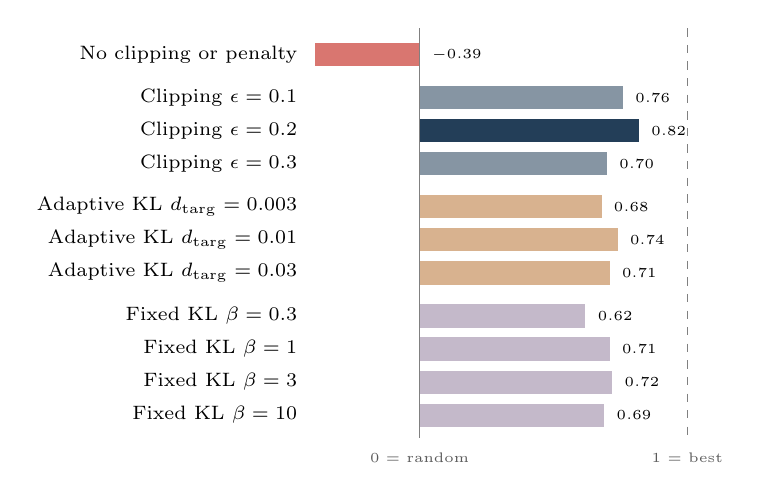
\begin{tikzpicture}[x=3.4cm, y=0.42cm, font=\scriptsize]
  \foreach \y/\lab/\v/\c in {
      0/No clipping or penalty/-0.39/BadRed!70,
      1.3/Clipping $\epsilon=0.1$/0.76/AtlasCool!55,
      2.3/Clipping $\epsilon=0.2$/0.82/AtlasCool,
      3.3/Clipping $\epsilon=0.3$/0.70/AtlasCool!55,
      4.6/Adaptive KL $d_{\mathrm{targ}}=0.003$/0.68/AtlasWarm!55,
      5.6/Adaptive KL $d_{\mathrm{targ}}=0.01$/0.74/AtlasWarm!55,
      6.6/Adaptive KL $d_{\mathrm{targ}}=0.03$/0.71/AtlasWarm!55,
      7.9/Fixed KL $\beta=0.3$/0.62/AtlasSlate!40,
      8.9/Fixed KL $\beta=1$/0.71/AtlasSlate!40,
      9.9/Fixed KL $\beta=3$/0.72/AtlasSlate!40,
      10.9/Fixed KL $\beta=10$/0.69/AtlasSlate!40} {
    \fill[\c] (0,-\y-0.35) rectangle (\v,-\y+0.35);
    \node[anchor=east] at (-0.42,-\y) {\lab};
    \node[anchor=west, font=\tiny] at ({max(\v,0)+0.01},-\y) {$\v$};}
  \draw[gray] (0,0.8) -- (0,-11.6);
  \draw[gray, dashed] (1,0.8) -- (1,-11.6);
  \node[font=\tiny, NoteGray] at (0,-12.2) {0 = random};
  \node[font=\tiny, NoteGray] at (1,-12.2) {1 = best};
\end{tikzpicture}\\
{\scriptsize PPO Table 1: 7 MuJoCo tasks $\times$ 3 seeds, 1M steps.}
\end{minipage}\hfill
\begin{minipage}[c]{0.42\linewidth}
\begin{warmbox}[title={Adaptive KL penalty}]
\begin{gather*}
  L^{KLPEN} = \hat\E_t\big[r_t\hat A_t - \beta\,\DKL[\pi_{\told},\pi_\theta]\big]
\end{gather*}
After each update, with $d=\hat\E_t[\DKL]$:
\begin{itemize}
  \item $d < d_{\mathrm{targ}}/1.5$: \ $\beta\leftarrow\beta/2$
  \item $d > 1.5\,d_{\mathrm{targ}}$: \ $\beta\leftarrow 2\beta$
\end{itemize}
{\scriptsize Constants 1.5 and 2 are heuristic; not sensitive to them.}
\end{warmbox}
\begin{keybox}
Clipping with $\epsilon=0.2$ wins; the KL penalty stays a useful baseline.
\end{keybox}
\end{minipage}

\subsection{PPO vs.\ other algorithms}

\begin{center}
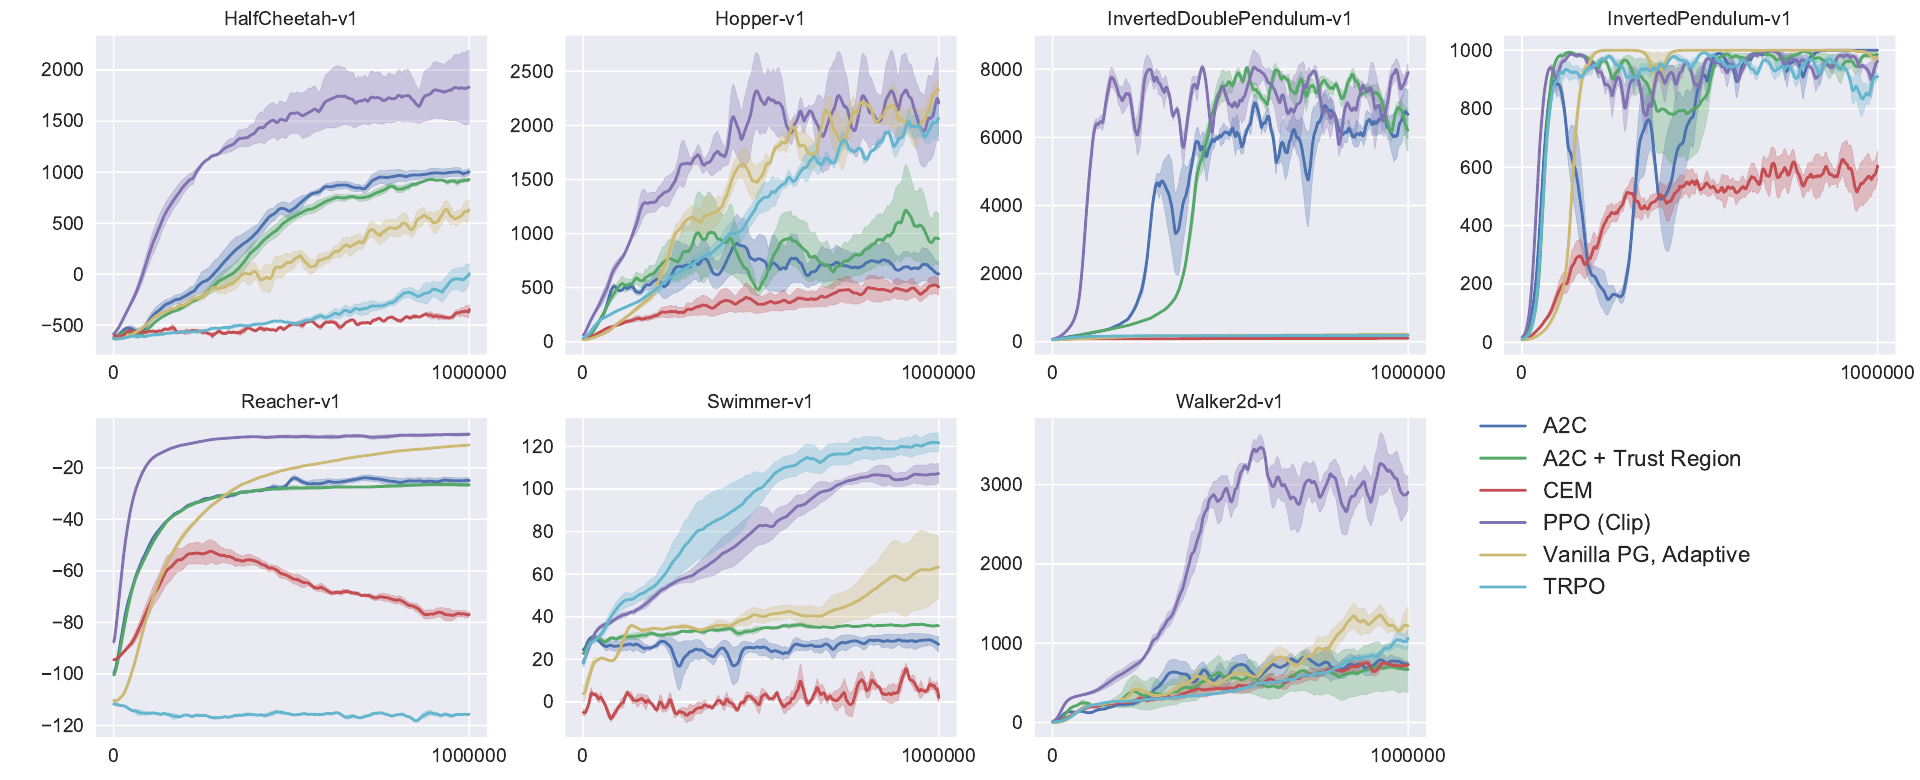
\includegraphics[width=\linewidth]{ppo_fig3_mujoco.png}\\
{\scriptsize PPO Fig.~3: MuJoCo, one million timesteps.}
\end{center}

\begin{minipage}[c]{0.5\linewidth}
\begin{itemize}
  \item \textbf{MuJoCo}: {\color{AtlasCool}\textbf{PPO (clip)}} best on almost all 7 tasks --- above TRPO, A2C, CEM, vanilla PG. Swimmer is the one task where TRPO is clearly ahead.
  \item Also (not shown): 3D humanoid running, steering and getting up.
\end{itemize}
\end{minipage}\hfill
\begin{minipage}[c]{0.46\linewidth}
\centering\small
\textbf{Atari}, 49 games --- games won\\[2pt]
\begin{tabular}{l r r r}
\toprule
 & A2C & ACER & \textbf{PPO} \\
\midrule
avg.\ over training & 1 & 18 & \textbf{30} \\
last 100 episodes & 1 & \textbf{28} & 19 \\
\bottomrule
\end{tabular}\\[2pt]
{\scriptsize ``avg.\ over training'' favors fast learning.}
\end{minipage}

% ---------------------------------------------------------------------------
\section{The whole story: CPI $\to$ TRPO $\to$ GAE $\to$ PPO}
% ---------------------------------------------------------------------------

\begin{center}
\footnotesize
\begin{tabularx}{\linewidth}{@{}>{\bfseries\raggedright\arraybackslash}p{2.6cm} L L L L@{}}
\toprule
 & \textbf{CPI} & \textbf{TRPO} & \textbf{GAE} & \textbf{PPO} \\
\midrule
{\color{AtlasWarm}A.\ how far may I step?} & mixture step $\alpha$ & KL trust region $\delta$ & trust region for $\pi$ \textbf{and} $V$ & clipped ratio $\epsilon$ \\
how is it solved? & greedy chooser + formula for $\alpha$ & CG + line search & CG (policy and value) & Adam, $K$ epochs \\
advantage estimate & rollouts from restarts & Monte Carlo $\hat Q$ & GAE$(\gamma,\lambda)$ + critic & truncated GAE \\
{\color{AtlasCool}B.\ where do states come from?} & {\color{AtlasCool}restarts $s_0\sim\mu$} & {\color{BadRed}$\rho_0$ (vine: resets to visited states)} & {\color{BadRed}$\rho_0$} & {\color{BadRed}$\rho_0$ (+ entropy bonus on actions)} \\
\bottomrule
\end{tabularx}
\end{center}

\begin{enumerate}
  \item \textbf{Row A}: the same idea at every stage --- keep the new policy close to the one that produced the data, because the surrogate uses the old state distribution. By construction (CPI), by a constraint (TRPO), by the objective (PPO).
  \item \textbf{Rows 2--3}: the price of keeping close falls, from a theoretical step size to an off-the-shelf optimizer, and from restart rollouts to a learned critic.
  \item \textbf{Row B}: CPI's second fix is \textbf{not} carried forward.
\end{enumerate}

\subsection{One line per paper}

\begin{center}
\small
\begin{tabularx}{\linewidth}{@{}l L L@{}}
\toprule
\textbf{Paper} & \textbf{Problem it attacks} & \textbf{Main idea} \\
\midrule
\textbf{CPI} & greedy updates from approximate values can hurt & conservative mixture, step $\alpha$ from a bound \\
\textbf{CPI} & on-policy samples miss important states & exploratory restart distribution $\mu$ \\
\textbf{TRPO} & mixtures don't fit neural-net policies & step size $=$ a policy distance (KL) \\
\textbf{TRPO} (practice) & the theoretical penalty is far too conservative & mean-KL trust region, CG + line search \\
{\color{AtlasWarm}\textbf{GAE}} & $\hat A_t$ from returns is too noisy & critic $V$ + bias--variance knob $\lambda$ \\
{\color{AtlasCool}\textbf{PPO}} & second-order step, one step per batch & clipped ratio + minibatch SGD, $K$ epochs \\
\bottomrule
\end{tabularx}
\end{center}

\begin{keybox}[title={Take-home}]
One idea --- \textbf{stay close to the data-generating policy, measured on its own states} --- runs from CPI to PPO, made cheaper at each step. CPI's state-coverage idea was dropped along the way.
\end{keybox}

% ===========================================================================
%  PART V --- RL FOR LANGUAGE MODELS
%  Human preferences -> InstructGPT -> DPO -> GRPO -> RLOO
% ===========================================================================
\clearpage
\part{RL for Language Models}

\partintro{\textbf{The question of Part V:} what does the CPI $\to$ PPO machinery look like when the ``environment'' is text and the reward is a learned model of human preferences? The part is organized around one question --- \textbf{what can we remove?} --- from InstructGPT's four models down to plain REINFORCE.}

% ---------------------------------------------------------------------------
\section{Text generation as an RL problem}
% ---------------------------------------------------------------------------

\begin{center}
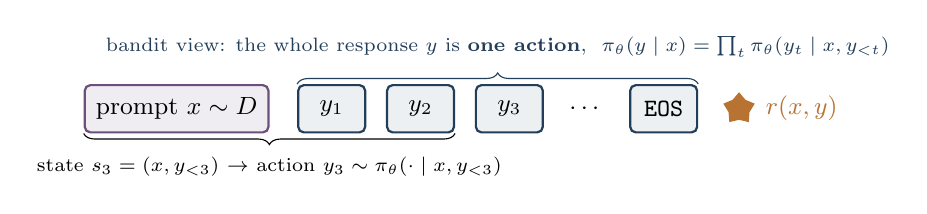
\begin{tikzpicture}[font=\small, >=Stealth,
    tok/.style={rectangle, rounded corners=2pt, draw=AtlasCool, thick, fill=AtlasCool!8,
      minimum width=0.85cm, minimum height=0.6cm, inner sep=1pt}]
  \node[rectangle, rounded corners=2pt, draw=AtlasSlate, thick, fill=AtlasSlate!10,
        minimum height=0.6cm, inner sep=4pt] (x) at (0,0) {prompt $x\sim D$};
  \node[tok, right=0.35cm of x] (y1) {$y_1$};
  \node[tok, right=0.25cm of y1] (y2) {$y_2$};
  \node[tok, right=0.25cm of y2] (y3) {$y_3$};
  \node[right=0.2cm of y3] (dots) {$\cdots$};
  \node[tok, right=0.2cm of dots] (eos) {\texttt{EOS}};
  \node[star, star points=5, fill=AtlasWarm, minimum size=0.42cm, inner sep=0pt, right=0.35cm of eos] (r) {};
  \node[right=0.05cm of r, font=\small, AtlasWarm] {$r(x,y)$};
  \draw[decorate, decoration={brace, amplitude=4pt, mirror}] (x.south west) -- (y2.south east)
    node[midway, below=5pt, font=\scriptsize]{state $s_3=(x,y_{<3})$ $\to$ action $y_3\sim\pi_\theta(\cdot\mid x,y_{<3})$};
  \draw[decorate, decoration={brace, amplitude=4pt}, AtlasCool] (y1.north west) -- (eos.north east)
    node[midway, above=6pt, font=\scriptsize]{bandit view: the whole response $y$ is \textbf{one action}, \ $\pi_\theta(y\mid x)=\prod_t\pi_\theta(y_t\mid x,y_{<t})$};
\end{tikzpicture}
\end{center}

\begin{pair}[3]
\begin{slatebox}[title={Start distribution $D$}]
\small The prompts users send --- ``$D$ comes from the application'' (Part~I).
\end{slatebox}
\begin{coolbox}[title={Dynamics}]
\small Append the token: \textbf{known} and \textbf{deterministic}.
\end{coolbox}
\begin{warmbox}[title={Reward}]
\small Only at the end --- but who writes $r(x,y)$ for ``helpful''?
\end{warmbox}
\end{pair}

\begin{notebox}
\begin{itemize}[leftmargin=*]
  \item Token-level MDP as in RLHF with PPO: discount 1, reward-model score at \texttt{EOS}, per-token KL elsewhere (RLOO paper, Sec.~2.1).
  \item InstructGPT calls it ``a bandit environment which presents a random customer prompt and expects a response'' (Sec.~3.5).
  \item Our remark: deterministic, known dynamics make resetting to any prefix free --- exactly what CPI's restarts $\mu$ and TRPO's vine needed. The open question is the \textbf{reward}.
\end{itemize}
\end{notebox}

\subsection{RLHF with PPO: what can we remove?}

\begin{center}
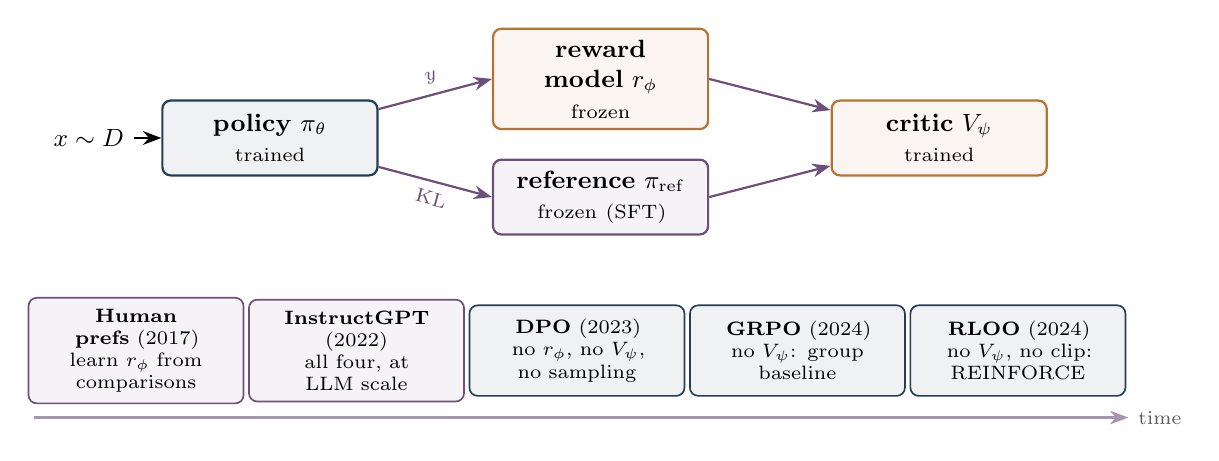
\begin{tikzpicture}[font=\small, >=Stealth,
    m/.style={fl, line width=0.8pt, text width=2.45cm, minimum height=0.95cm},
    p/.style={fl, line width=0.6pt, text width=2.45cm, minimum height=1.15cm, font=\scriptsize}]
  \node (x) at (-6.2,0) {$x\sim D$};
  \node[m, cbox=AtlasCool] (pi) at (-3.9,0) {\textbf{policy} $\pi_\theta$\\ {\scriptsize trained}};
  \node[m, cbox=AtlasWarm] (rm) at (0.3,0.75) {\textbf{reward model} $r_\phi$\\ {\scriptsize frozen}};
  \node[m, cbox=AtlasSlate] (ref) at (0.3,-0.75) {\textbf{reference} $\pi_{\mathrm{ref}}$\\ {\scriptsize frozen (SFT)}};
  \node[m, cbox=AtlasWarm] (v) at (4.6,0) {\textbf{critic} $V_\psi$\\ {\scriptsize trained}};
  \draw[->, thick] (x) -- (pi);
  \draw[->, thick, AtlasSlate] (pi) -- node[above, font=\scriptsize, sloped]{$y$} (rm.west);
  \draw[->, thick, AtlasSlate] (pi) -- node[below, font=\scriptsize, sloped]{KL} (ref.west);
  \draw[->, thick, AtlasSlate] (rm.east) -- (v);
  \draw[->, thick, AtlasSlate] (ref.east) -- (v);
  \node[p, cbox=AtlasSlate] (t1) at (-5.6,-2.7) {\textbf{Human prefs} (2017)\\ learn $r_\phi$ from comparisons};
  \node[p, cbox=AtlasSlate] (t2) at (-2.8,-2.7) {\textbf{InstructGPT} (2022)\\ all four, at LLM scale};
  \node[p, cbox=AtlasCool] (t3) at (0,-2.7) {\textbf{DPO} (2023)\\ no $r_\phi$, no $V_\psi$, no sampling};
  \node[p, cbox=AtlasCool] (t4) at (2.8,-2.7) {\textbf{GRPO} (2024)\\ no $V_\psi$: group baseline};
  \node[p, cbox=AtlasCool] (t5) at (5.6,-2.7) {\textbf{RLOO} (2024)\\ no $V_\psi$, no clip: REINFORCE};
  \draw[->, thick, AtlasSlate!60] (-6.9,-3.55) -- (7.0,-3.55) node[right, font=\scriptsize, NoteGray]{time};
\end{tikzpicture}
\end{center}

{\small PPO for RLHF ``typically requires loading up to 4 models simultaneously: the generator, the reference (for KL estimation), the critic, and the reward model'' (RLOO paper, Sec.~1). In InstructGPT the critic is initialized from the reward model (6B each).}

% ---------------------------------------------------------------------------
\section{Learning the reward from human preferences}
% ---------------------------------------------------------------------------

\paper{Deep Reinforcement Learning from Human Preferences}
  {Christiano, Leike, Brown, Martic, Legg \& Amodei}{NeurIPS 2017}
  {a reward model learned from pairwise human comparisons}
  {rlhf.md}

\begin{enumerate}
  \item Observations $o_t$, actions $a_t$ (Atari, MuJoCo) --- \textbf{no reward} from the environment.
  \item A human compares two short clips $\sigma^1,\sigma^2$ (1--2\,s): which is better?
  \item Goal: behavior the human prefers, with \textbf{few} queries.
  \item No resets to chosen states: clips start wherever the agent was.
  \item The policy is trained by any RL method: \textbf{TRPO} (MuJoCo), \textbf{A2C} (Atari).
\end{enumerate}

{\small Motivation: tasks we can recognize but not demonstrate or specify (a backflip). Comparisons were easier for humans than absolute scores.}

\subsection{Three processes, running asynchronously}

\begin{minipage}[c]{0.52\linewidth}
\centering
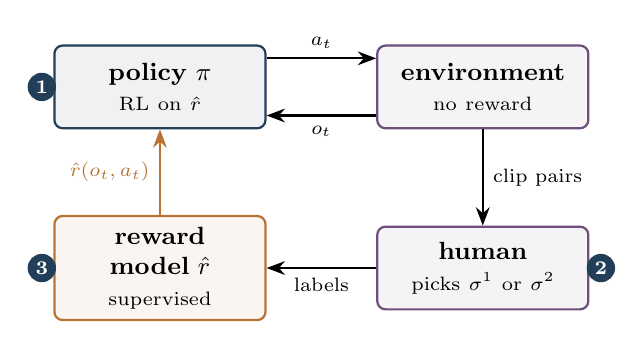
\begin{tikzpicture}[font=\small, >=Stealth,
    m/.style={fl, line width=0.8pt, text width=2.4cm, minimum height=1.05cm},
    num/.style={circle, fill=AtlasAccent, text=white, font=\scriptsize\bfseries, inner sep=1pt, minimum size=0.36cm}]
  \node[m, cbox=AtlasCool] (pi) at (0,2.3) {\textbf{policy} $\pi$\\ {\scriptsize RL on $\hat r$}};
  \node[m, cbox=AtlasSlate] (env) at (4.1,2.3) {\textbf{environment}\\ {\scriptsize no reward}};
  \node[m, cbox=AtlasSlate] (hum) at (4.1,0) {\textbf{human}\\ {\scriptsize picks $\sigma^1$ or $\sigma^2$}};
  \node[m, cbox=AtlasWarm] (rhat) at (0,0) {\textbf{reward model} $\hat r$\\ {\scriptsize supervised}};
  \draw[->, thick] (pi.15) -- node[above, font=\scriptsize]{$a_t$} (env.165);
  \draw[->, thick] (env.195) -- node[below, font=\scriptsize]{$o_t$} (pi.345);
  \draw[->, thick] (env) -- node[right, font=\scriptsize]{clip pairs} (hum);
  \draw[->, thick] (hum) -- node[below, font=\scriptsize]{labels} (rhat);
  \draw[->, thick, AtlasWarm] (rhat) -- node[left, font=\scriptsize]{$\hat r(o_t,a_t)$} (pi);
  \node[num] at (-1.5,2.3) {1};
  \node[num] at (5.6,0) {2};
  \node[num] at (-1.5,0) {3};
\end{tikzpicture}
\end{minipage}\hfill
\begin{minipage}[c]{0.45\linewidth}
\begin{enumerate}
  \item RL maximizes the \textbf{predicted} reward $\sum_t\hat r(o_t,a_t)$.
  \item Pairs of clips go to the human.
  \item $\hat r$ is fit to all comparisons so far.
\end{enumerate}
\end{minipage}

\begin{pair}
\begin{keybox}[title={Few labels}]
Feedback on $<1\%$ of interactions. MuJoCo: 700 labels $\approx$ RL with the true reward. Backflip: 900 queries, $<1$ hour.
\end{keybox}
\begin{warnbox}[title={Keep feedback in the loop}]
Training $\hat r$ only on early queries fails: the policy \textbf{exploits} the partial reward (e.g.\ endless volleys in Pong).
\end{warnbox}
\end{pair}

{\small Queries are chosen where an ensemble of reward predictors disagrees most. Rewards from $\hat r$ are normalized to zero mean (only differences are identified).}

\subsection{Fitting the reward: the Bradley--Terry model}

\begin{minipage}[c]{0.55\linewidth}
Preference $=$ logistic in the \textbf{difference} of summed rewards:
\begin{gather*}
  \hat P[\sigma^1\succ\sigma^2]
  = \frac{e^{\sum_t\hat r(o_t^1,a_t^1)}}{e^{\sum_t\hat r(o_t^1,a_t^1)}+e^{\sum_t\hat r(o_t^2,a_t^2)}}
  = \sigma\big(\hat R(\sigma^1)-\hat R(\sigma^2)\big)
\end{gather*}
\end{minipage}\hfill
\begin{minipage}[c]{0.4\linewidth}
\centering
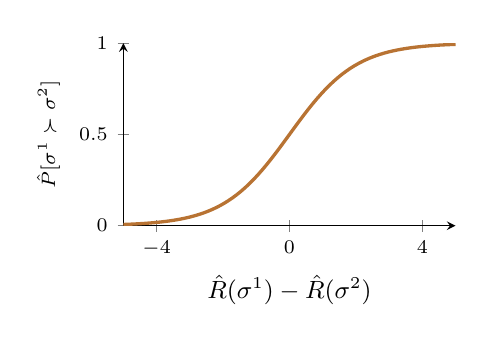
\begin{tikzpicture}
\begin{axis}[notes, width=5.8cm, height=3.9cm, xmin=-5, xmax=5, ymin=0, ymax=1,
    xlabel={$\hat R(\sigma^1)-\hat R(\sigma^2)$}, ytick={0,0.5,1}, xtick={-4,0,4},
    ylabel={$\hat P[\sigma^1\succ\sigma^2]$}, ylabel style={font=\scriptsize}]
  \addplot[AtlasWarm, very thick, domain=-5:5, samples=80] {1/(1+exp(-x))};
\end{axis}
\end{tikzpicture}\\
{\scriptsize Like \textbf{Elo} in chess: the rating gap predicts who wins.}
\end{minipage}

Fit $\hat r$ by cross-entropy on the labels $\mu$ (all mass on the preferred clip, uniform if ``equally good''):
\begin{eqbox}
\begin{gather*}
  \mathrm{loss}(\hat r) = -\sum_{\mathcal D}\Big[\mu(1)\log\hat P[\sigma^1\succ\sigma^2] + \mu(2)\log\hat P[\sigma^2\succ\sigma^1]\Big]
\end{gather*}
\end{eqbox}

\begin{keybox}[title={Only differences matter}]
$\hat r+c$ fits equally well $\Rightarrow$ normalize. \textbf{This invariance is what DPO exploits.} For LLMs the clips become responses $y$ to the same prompt $x$.
\end{keybox}

% ---------------------------------------------------------------------------
\section{InstructGPT: RLHF at LLM scale}
% ---------------------------------------------------------------------------

\paper{Training Language Models to Follow Instructions with Human Feedback}
  {Ouyang, Wu, Jiang, et al.\ (OpenAI)}{NeurIPS 2022}
  {InstructGPT --- the SFT $\to$ reward model $\to$ PPO recipe}
  {2203.02155v1.pdf}

\begin{enumerate}
  \item $D$: real prompts sent to the OpenAI API, plus labeler-written ones.
  \item \textbf{Bandit} environment: a prompt, a response, a reward from the RM, end of episode.
  \item Rewards from a 6B \textbf{reward model} trained on labeler rankings.
  \item Per-token \textbf{KL penalty} to the SFT model.
  \item GPT-3 architecture: 1.3B, 6B, 175B.
\end{enumerate}

\subsection{The three-step recipe}

\begin{pair}[3]
\begin{slatebox}[title={1. SFT}]
\small
\begin{itemize}
  \item Labelers \textbf{write} answers.
  \item Supervised fine-tuning of GPT-3.
  \item {\color{NoteGray}13k prompts}
\end{itemize}
\end{slatebox}
\begin{warmbox}[title={2. Reward model}]
\small
\begin{itemize}
  \item Labelers \textbf{rank} $K=4$--$9$ outputs $\to\binom K2$ pairs.
  \item Loss $-\log\sigma\big(r_\theta(x,y_w)-r_\theta(x,y_l)\big)$.
  \item {\color{NoteGray}33k prompts; 6B RM}
\end{itemize}
\end{warmbox}
\begin{coolbox}[title={3. PPO}]
\small
\begin{itemize}
  \item New prompt $\to$ the policy writes $y$.
  \item RM scores $y$ $\to$ PPO step (critic initialized from the RM).
  \item {\color{NoteGray}31k prompts, API only}
\end{itemize}
\end{coolbox}
\end{pair}

\begin{defbox}{reward-model loss (InstructGPT Eq.~1)}
\begin{gather*}
  \mathrm{loss}(\theta)=-\frac{1}{\binom K2}\E_{(x,y_w,y_l)\sim D}\Big[\log\sigma\big(r_\theta(x,y_w)-r_\theta(x,y_l)\big)\Big]
\end{gather*}
The Bradley--Terry loss of the previous section, with responses instead of clips.
\end{defbox}

\begin{notebox}
\begin{itemize}[leftmargin=*]
  \item \textbf{All $\binom K2$ pairs in one batch element}: treating them as separate data points made each completion appear in $K-1$ updates, and the RM overfit after one epoch.
  \item The RM is the SFT model with the unembedding layer replaced by a scalar head; 175B RMs were unstable, so all RMs are 6B.
  \item SFT: 16 epochs --- overfits validation loss after 1 epoch, but more epochs help RM score and human ratings.
\end{itemize}
\end{notebox}

\subsection{The KL-regularized objective (PPO-ptx)}

\begin{eqbox}
\begin{gather*}
  \mathrm{objective}(\phi) =
  \E_{(x,y)\sim D_{\pi_\phi^{RL}}}\Big[\underbrace{r_\theta(x,y)}_{\text{\color{AtlasWarm}reward model}}
    - \underbrace{\beta\log\frac{\pi_\phi^{RL}(y\mid x)}{\pi^{SFT}(y\mid x)}}_{\text{\color{AtlasSlate}stay near SFT}}\Big]
  + \underbrace{\gamma\,\E_{x\sim D_{\mathrm{pre}}}\big[\log\pi_\phi^{RL}(x)\big]}_{\text{\color{AtlasCool}pretraining mix}}
\end{gather*}
\end{eqbox}

\begin{pair}[3]
\begin{warmbox}[title={Reward}]
\small The RM is only a \textbf{proxy} for the labelers.
\end{warmbox}
\begin{slatebox}[title={KL, $\beta=0.02$}]
\small Per token, against \textbf{over-optimizing} the RM. Its expectation is $\DKL(\pi^{RL}\|\pi^{SFT})$.
\end{slatebox}
\begin{coolbox}[title={ptx, $\gamma>0$}]
\small Fixes the ``alignment tax'' on public NLP benchmarks (SQuAD, DROP, HellaSwag, WMT).
\end{coolbox}
\end{pair}

\begin{keybox}[title={Results}]
Labelers prefer the \textbf{1.3B} InstructGPT to the \textbf{175B} GPT-3. 175B vs.\ 175B: preferred $85\pm3\%$ of the time. TruthfulQA about twice GPT-3; closed-domain hallucination 21\% vs.\ 41\%.
\end{keybox}

\begin{notebox}
Without ptx ($\gamma=0$) this is the RLHF objective that \textbf{DPO} starts from. Here $\gamma$ is a mixing weight, not a discount. ``PPO'' models: $\gamma=0$; ``PPO-ptx'': $\gamma>0$. The paper aligns GPT-3 ``to the stated preferences of a specific group of people (mostly our labelers and researchers)'', not to broader human values (Sec.~5.2).
\end{notebox}

% ---------------------------------------------------------------------------
\section{DPO: the RLHF objective as a classification loss}
% ---------------------------------------------------------------------------

\paper{Direct Preference Optimization: Your Language Model Is Secretly a Reward Model}
  {Rafailov, Sharma, Mitchell, Ermon, Manning \& Finn}{NeurIPS 2023}
  {DPO --- the RLHF objective solved with a classification loss}
  {dpo/dpo.md}

\begin{enumerate}
  \item Same objective as RLHF: reward minus $\beta\,\DKL(\pi\,\|\,\pi_{\mathrm{ref}})$, with $\pi_{\mathrm{ref}}=\pi^{SFT}$.
  \item Preferences follow \textbf{Bradley--Terry} with a latent reward $r^*$.
  \item A \textbf{fixed} dataset $\mathcal D=\{(x,y_w,y_l)\}$ (offline).
  \item No reward model, \textbf{no sampling} from $\pi_\theta$ during training, no critic.
\end{enumerate}

\subsection{From the RLHF objective to a loss on the policy}

Four steps.

\begin{enumerate}
  \item \textbf{The RLHF objective}, for a reward $r$:
  \begin{gather*}
    \max_\pi\ \E_{x,\,y\sim\pi}\big[r(x,y)\big] - \beta\,\DKL\big[\pi\,\|\,\pi_{\mathrm{ref}}\big]
  \end{gather*}
  \item \textbf{Its optimum in closed form} --- tilt $\pi_{\mathrm{ref}}$ by $e^{r/\beta}$:
  \begin{gather*}
    \pi_r(y\mid x) = \frac{1}{Z(x)}\,\pi_{\mathrm{ref}}(y\mid x)\,e^{r(x,y)/\beta}, \qquad Z(x)=\textstyle\sum_y\pi_{\mathrm{ref}}(y\mid x)\,e^{r(x,y)/\beta}
  \end{gather*}
  {\small Why: the objective equals $-\beta\,\DKL(\pi\|\pi_r)+\beta\log Z(x)$, minimized at $\pi=\pi_r$ (DPO App.~A.1). $Z(x)$ is intractable.}
  \item \textbf{Solve for the reward}:
  \begin{gather*}
    r(x,y) = \beta\log\frac{\pi_r(y\mid x)}{\pi_{\mathrm{ref}}(y\mid x)} + \beta\log Z(x)
  \end{gather*}
  \item \textbf{Into Bradley--Terry}: both responses share $x$, so $\beta\log Z(x)$ \textbf{cancels}:
\end{enumerate}

\begin{eqbox}
\begin{gather*}
  \mathcal L_{\mathrm{DPO}} = -\E_{\mathcal D}\Big[\log\sigma\big(\hat r_\theta(x,y_w) - \hat r_\theta(x,y_l)\big)\Big],
  \qquad \hat r_\theta(x,y) = \beta\log\frac{\pi_\theta(y\mid x)}{\pi_{\mathrm{ref}}(y\mid x)}
\end{gather*}
\end{eqbox}

\begin{minipage}[c]{0.5\linewidth}
\centering
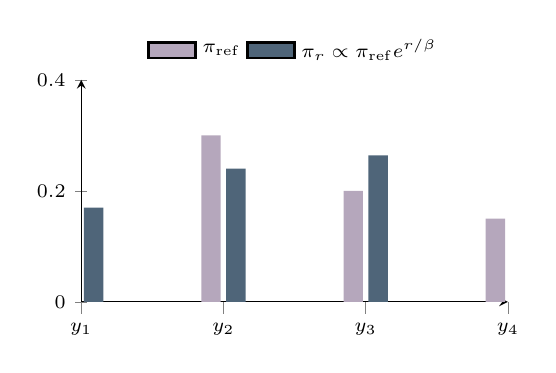
\begin{tikzpicture}
\begin{axis}[notes, width=7cm, height=4.4cm, ybar, bar width=7pt, ymin=0, ymax=0.4,
    xtick={1,2,3,4}, xticklabels={$y_1$,$y_2$,$y_3$,$y_4$}, ytick={0,0.2,0.4},
    legend style={at={(0.5,1.03)}, anchor=south, legend columns=2}, area legend]
  \addplot[fill=AtlasSlate!50, draw=none] coordinates {(1,0.35)(2,0.30)(3,0.20)(4,0.15)};
  \addlegendentry{$\pi_{\mathrm{ref}}$}
  \addplot[fill=AtlasCool!80, draw=none] coordinates {(1,0.170)(2,0.240)(3,0.264)(4,0.326)};
  \addlegendentry{$\pi_r\propto\pi_{\mathrm{ref}}e^{r/\beta}$}
\end{axis}
\end{tikzpicture}\\
{\scriptsize Toy example: $\beta=1$, rewards $r=0,\,0.5,\,1,\,1.5$. High-reward answers gain mass.}
\end{minipage}\hfill
\begin{minipage}[c]{0.46\linewidth}
\begin{keybox}[title={Read it backwards}]
\textbf{Every policy defines a reward}, $\hat r_\theta=\beta\log\frac{\pi_\theta}{\pi_{\mathrm{ref}}}$, up to a term that depends on $x$ only. The reward-model loss with $r_\phi$ replaced by $\hat r_\theta$: \textbf{the LM is the reward model}.
\end{keybox}
\end{minipage}

\begin{notebox}
Thm.~1 of DPO: the reparameterization loses no generality --- every reward class (rewards equal up to a function of $x$) contains one of the form $\beta\log\pi/\pi_{\mathrm{ref}}$. Link to Part~I: the optimum is a \emph{soft-greedy} policy, and $Z(x)$ plays the role of a soft value of $\pi_{\mathrm{ref}}$. DPO also works with Plackett--Luce rankings (App.~A.3), i.e.\ InstructGPT-style $K$-way rankings.
\end{notebox}

\subsection{What the DPO update does}

\begin{gather*}
  \nabla_\theta\mathcal L_{\mathrm{DPO}} = -\beta\,\E_{\mathcal D}\Big[
    \underbrace{\sigma\big(\hat r_\theta(x,y_l)-\hat r_\theta(x,y_w)\big)}_{\text{\color{AtlasWarm}large when the ranking is wrong}}
    \big(\underbrace{\nabla_\theta\log\pi_\theta(y_w\mid x)}_{\text{raise }y_w} - \underbrace{\nabla_\theta\log\pi_\theta(y_l\mid x)}_{\text{lower }y_l}\big)\Big]
\end{gather*}

\begin{minipage}[c]{0.45\linewidth}
\centering
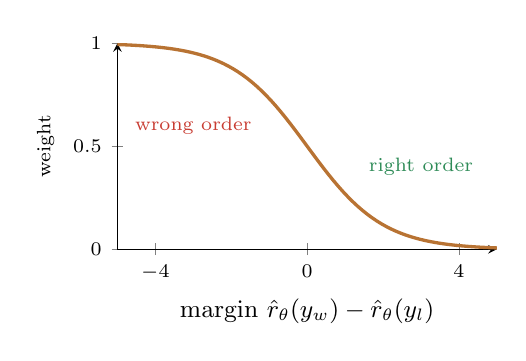
\begin{tikzpicture}
\begin{axis}[notes, width=6.4cm, height=4.2cm, xmin=-5, xmax=5, ymin=0, ymax=1,
    xlabel={margin $\hat r_\theta(y_w)-\hat r_\theta(y_l)$}, ytick={0,0.5,1}, xtick={-4,0,4},
    ylabel={weight}, ylabel style={font=\scriptsize}]
  \addplot[AtlasWarm, very thick, domain=-5:5, samples=80] {1/(1+exp(x))};
  \node[font=\scriptsize, BadRed] at (axis cs:-3,0.6) {wrong order};
  \node[font=\scriptsize, GoodGreen] at (axis cs:3,0.4) {right order};
\end{axis}
\end{tikzpicture}
\end{minipage}\hfill
\begin{minipage}[c]{0.52\linewidth}
\begin{itemize}
  \item Like the reward-model loss --- applied to the policy itself.
  \item The weight \textbf{fades} once a pair is ranked right. Without it (unlikelihood: equal weights) the model \textbf{degenerates}.
  \item \textbf{Sentiment} (IMDb): best reward for every KL budget, above PPO --- even PPO with the true reward.
  \item \textbf{TL;DR}: 61\% win rate vs.\ PPO's 57\%; more robust to sampling temperature.
\end{itemize}
\end{minipage}

\subsection{What we removed, and what it costs}

\begin{pair}
\begin{keybox}[title={Removed}]
\begin{itemize}
  \item The reward model --- implicit in $\pi_\theta$.
  \item The critic and the RL loop.
  \item Sampling during training.
\end{itemize}
Left: $\pi_\theta$, $\pi_{\mathrm{ref}}$ and one supervised-style loss. Same optimum as RLHF (under Bradley--Terry).
\end{keybox}
\begin{warnbox}[title={Costs}]
\begin{itemize}
  \item \textbf{Offline}: responses come from $\pi^{SFT}$, not $\pi_\theta$ --- no exploration.
  \item Learns only on the pairs in $\mathcal D$.
  \item Later evidence: online beats offline (DeepSeekMath); DPO answers are long (RLOO paper: 104 tokens vs.\ 60.6 for RLOO on HH).
\end{itemize}
\end{warnbox}
\end{pair}

\begin{notebox}
\textbf{Part I echo:} CPI's quality depends on how well the sampling distribution covers the good states ($\|d_{\pi^*}/\mu\|_\infty$, Thm.~6.2). Here: how well $\pi^{SFT}$'s answers cover good answers. (Our analogy; the DPO paper itself does not state these costs in this form.)
\end{notebox}

% ---------------------------------------------------------------------------
\section{GRPO: PPO without the critic}
% ---------------------------------------------------------------------------

\paper{DeepSeekMath: Pushing the Limits of Mathematical Reasoning in Open Language Models}
  {Shao, Wang, Zhu, et al.\ (DeepSeek-AI)}{arXiv 2024}
  {GRPO --- PPO with a group baseline instead of a critic}
  {deepseekmat\_pushing\_the\_limits\_of\_\ldots.md}

\begin{enumerate}
  \item Math questions $q$ (GSM8K, MATH; chain of thought); policy: DeepSeekMath-Instruct 7B.
  \item A \textbf{reward model} scores each output $o$ --- at the end (outcome) or per step (process).
  \item Online: $G=64$ outputs per question from the current policy.
  \item The problem with PPO's critic: \textbf{as large as the policy}, and hard to fit per token when the reward comes only at the end.
\end{enumerate}

{\small Most of the paper is about pre-training data (120B math tokens); GRPO is Sec.~4. KL coefficient 0.04, learning rate $10^{-6}$, batch 1024. GRPO later became the RL algorithm of DeepSeek-R1.}

\subsection{Group-relative advantages}

\begin{minipage}[c]{0.5\linewidth}
\centering
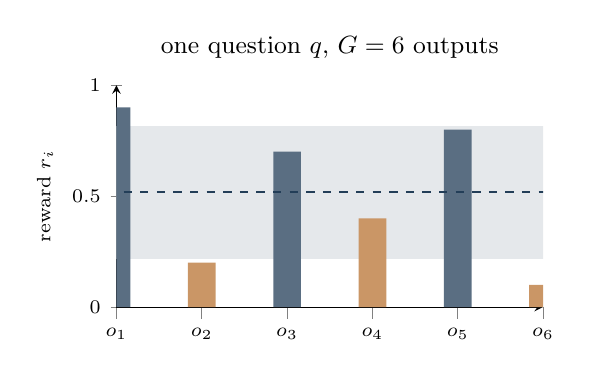
\begin{tikzpicture}
\begin{axis}[notes, width=7cm, height=4.4cm, ybar, bar width=10pt, ymin=0, ymax=1,
    xtick={1,...,6}, xticklabels={$o_1$,$o_2$,$o_3$,$o_4$,$o_5$,$o_6$}, ytick={0,0.5,1},
    ylabel={reward $r_i$}, ylabel style={font=\scriptsize}, title={\small one question $q$, $G=6$ outputs}]
  \fill[AtlasAccent!12] (axis cs:0.5,0.215) rectangle (axis cs:6.5,0.818);
  \addplot[fill=AtlasCool!75, draw=none, bar shift=0pt] coordinates {(1,0.9)(3,0.7)(5,0.8)};
  \addplot[fill=AtlasWarm!75, draw=none, bar shift=0pt] coordinates {(2,0.2)(4,0.4)(6,0.1)};
  \draw[AtlasAccent, thick, dashed] (axis cs:0.5,0.517) -- (axis cs:6.5,0.517);
  \node[font=\scriptsize, AtlasAccent, anchor=west] at (axis cs:6.5,0.517) {mean};
  \node[font=\scriptsize, AtlasAccent, anchor=west] at (axis cs:6.5,0.818) {$+$std};
\end{axis}
\end{tikzpicture}\\
{\scriptsize Toy rewards. Blue: above the mean (pushed up). Copper: below (pushed down).}
\end{minipage}\hfill
\begin{minipage}[c]{0.47\linewidth}
Sample $G$ outputs for the \textbf{same} question and score them:
\begin{eqbox}
\begin{gather*}
  \hat A_{i,t} = \frac{r_i - \mathrm{mean}(\mathbf r)}{\mathrm{std}(\mathbf r)}
\end{gather*}
\end{eqbox}
{\small The same value for every token $t$ of $o_i$ (outcome supervision).}
\begin{itemize}
  \item The group mean replaces $V(q)$: a critic computed \textbf{on the fly}.
  \item Matches how RMs are trained: \textbf{comparisons} within one question.
\end{itemize}
\end{minipage}

\begin{keybox}[title={Results}]
RL on GSM8K + MATH questions only: GSM8K $82.9\to88.2\%$, MATH $46.8\to51.7\%$, and gains out of domain (CMATH $84.6\to88.8\%$).
\end{keybox}

\begin{notebox}
\textbf{Process supervision} (Sec.~4.1.3): normalize per-step rewards across the group; token $t$ gets the sum of normalized rewards of the steps ending at or after $t$. It did better than outcome supervision. Sec.~5.2.2: RL improves Maj@K but not Pass@K --- it makes the output distribution more robust rather than adding new abilities.
\end{notebox}

\subsection{PPO vs.\ GRPO}

\begin{center}
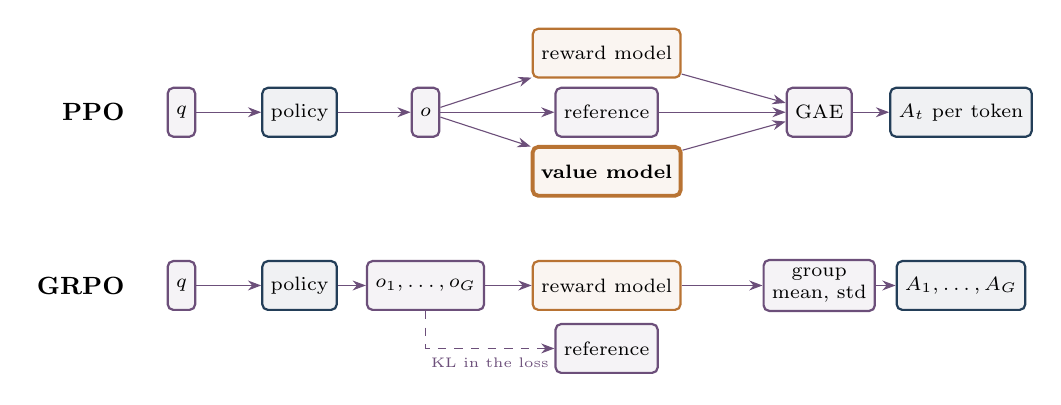
\begin{tikzpicture}[font=\scriptsize, >=Stealth,
    b/.style={rectangle, rounded corners=2pt, thick, minimum height=0.62cm, align=center, inner sep=3pt}]
  \node[font=\small\bfseries, anchor=east] at (-0.3,0) {PPO};
  \node[b, cbox=AtlasSlate] (q1) at (0.3,0) {$q$};
  \node[b, cbox=AtlasCool] (p1) at (1.8,0) {policy};
  \node[b, cbox=AtlasSlate] (o1) at (3.4,0) {$o$};
  \node[b, cbox=AtlasWarm] (r1) at (5.7,0.75) {reward model};
  \node[b, cbox=AtlasSlate] (f1) at (5.7,0) {reference};
  \node[b, cbox=AtlasWarm, line width=1.4pt] (v1) at (5.7,-0.75) {\textbf{value model}};
  \node[b, cbox=AtlasSlate] (g1) at (8.4,0) {GAE};
  \node[b, cbox=AtlasCool] (a1) at (10.2,0) {$A_t$ per token};
  \foreach \x/\y in {q1/p1, p1/o1, o1/r1, o1/f1, o1/v1, r1/g1, f1/g1, v1/g1, g1/a1} \draw[->, AtlasSlate] (\x) -- (\y);
  \node[font=\small\bfseries, anchor=east] at (-0.3,-2.2) {GRPO};
  \node[b, cbox=AtlasSlate] (q2) at (0.3,-2.2) {$q$};
  \node[b, cbox=AtlasCool] (p2) at (1.8,-2.2) {policy};
  \node[b, cbox=AtlasSlate] (o2) at (3.4,-2.2) {$o_1,\dots,o_G$};
  \node[b, cbox=AtlasWarm] (r2) at (5.7,-2.2) {reward model};
  \node[b, cbox=AtlasSlate] (g2) at (8.4,-2.2) {group\\ mean, std};
  \node[b, cbox=AtlasCool] (a2) at (10.2,-2.2) {$A_1,\dots,A_G$};
  \node[b, cbox=AtlasSlate] (f2) at (5.7,-3.0) {reference};
  \foreach \x/\y in {q2/p2, p2/o2, o2/r2, r2/g2, g2/a2} \draw[->, AtlasSlate] (\x) -- (\y);
  \draw[->, AtlasSlate, dashed] (o2) |- node[pos=0.75, below, font=\tiny]{KL in the loss} (f2);
\end{tikzpicture}
\end{center}

\begin{eqbox}
\begin{gather*}
  \mathcal J_{\mathrm{GRPO}}(\theta) = \E\Big[\frac1G\sum_{i=1}^G\frac{1}{|o_i|}\sum_{t=1}^{|o_i|}
    \Big\{\min\big(\rho_{i,t}\hat A_{i,t},\ \mathrm{clip}(\rho_{i,t},1\pm\varepsilon)\,\hat A_{i,t}\big)
    - \beta\,\DKL\big[\pi_\theta\|\pi_{\mathrm{ref}}\big]\Big\}\Big]
\end{gather*}
\end{eqbox}
{\small $\rho_{i,t}=\pi_\theta(o_{i,t}\mid q,o_{i,<t})/\pi_{\told}(o_{i,t}\mid q,o_{i,<t})$: still PPO's clipped ratio, per token.}

\begin{enumerate}
  \item \textbf{Critic gone}: the group statistics replace $V_\psi$ and GAE.
  \item \textbf{KL moved}: PPO for LLMs adds the per-token KL to the reward, so it passes through GAE; GRPO puts it in the loss, which keeps $\hat A$ simple. KL estimator (``k3''): $\frac{\pi_{\mathrm{ref}}}{\pi_\theta}-\log\frac{\pi_{\mathrm{ref}}}{\pi_\theta}-1\ge0$, unbiased under samples from $\pi_\theta$.
\end{enumerate}

\begin{warnbox}[title={The clip never acts in their runs}]
``The policy model only has a single update following each exploration stage'' (Sec.~4.2), so $\pi_\theta=\pi_{\told}$ when the gradient is taken: the ratio is 1 and the clip is inactive --- the gradient is \textbf{REINFORCE with a group baseline}. Iterative GRPO (Alg.~1) also retrains the RM and resets $\pi_{\mathrm{ref}}\leftarrow\pi_\theta$ between rounds.
\end{warnbox}

% ---------------------------------------------------------------------------
\section{RLOO: back to REINFORCE}
% ---------------------------------------------------------------------------

\paper{Back to Basics: Revisiting REINFORCE-Style Optimization for Learning from Human Feedback in LLMs}
  {Ahmadian, Cremer, Gall\'e, et al.\ (Cohere)}{ACL 2024}
  {REINFORCE with a leave-one-out baseline beats PPO for RLHF}
  {REINFORCE\_leave\_1\_out/}

\begin{enumerate}
  \item Standard RLHF: SFT $\to$ reward model $r_\phi$ $\to$ online RL.
  \item KL-shaped reward per response: $R(x,y)=r_\phi(x,y)-\beta\log\frac{\pi_\theta(y\mid x)}{\pi_{\mathrm{ref}}(y\mid x)}$.
  \item \textbf{Claim}: PPO's tools fight high variance from a \textbf{weak} start. A pretrained LLM is a \textbf{strong} start.
  \item Reward only at \texttt{EOS}, deterministic dynamics $\Rightarrow$ treat $y$ as \textbf{one action}.
\end{enumerate}

{\small ``Strong initialization coupled with prompt conditioning leads to the concentration of probability mass on a few tokens at each generation step'' (Sec.~3.1). Models: Pythia 6.9B, Llama-7B; data: TL;DR and Anthropic-HH.}

\subsection{Which parts of PPO does RLHF need?}

\begin{minipage}[c]{0.44\linewidth}
\centering
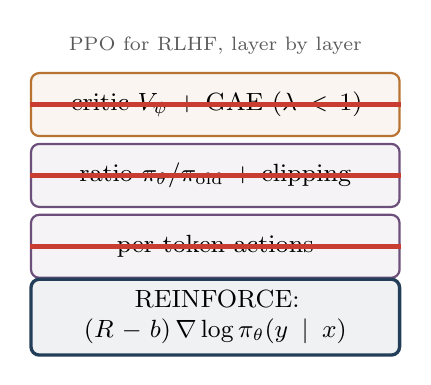
\begin{tikzpicture}[font=\small,
    layer/.style={fl, line width=0.8pt, text width=4.4cm, minimum height=0.8cm},
    strike/.style={BadRed, line width=1.6pt}]
  \node[font=\scriptsize, NoteGray] at (0,3.45) {PPO for RLHF, layer by layer};
  \node[layer, cbox=AtlasWarm] (l1) at (0,2.7) {critic $V_\psi$ + GAE ($\lambda<1$)};
  \node[layer, cbox=AtlasSlate] (l2) at (0,1.8) {ratio $\pi_\theta/\pi_{\mathrm{old}}$ + clipping};
  \node[layer, cbox=AtlasSlate] (l3) at (0,0.9) {per-token actions};
  \node[layer, cbox=AtlasCool, line width=1.2pt] (l0) at (0,0) {REINFORCE: $(R-b)\,\nabla\log\pi_\theta(y\mid x)$};
  \draw[strike] (l1.west) -- (l1.east);
  \draw[strike] (l2.west) -- (l2.east);
  \draw[strike] (l3.west) -- (l3.east);
\end{tikzpicture}
\end{minipage}\hfill
\begin{minipage}[c]{0.53\linewidth}
\begin{enumerate}
  \item \textbf{\color{AtlasWarm}Bias for variance? Not worth it.} Reward falls steadily as $\lambda$ goes $1\to0$; $\lambda=1$ (no bootstrapping) is best.
  \item \textbf{Clipping? Rarely active.} Clipped in $<5\%$ of each batch; removing ratio and clip does not hurt (``if anything a slight boost'').
  \item \textbf{Tokens as actions? Not needed.} The whole response as one action works as well or better.
\end{enumerate}
\end{minipage}

\begin{notebox}
Callback to Parts III--IV: these are exactly the tools GAE and PPO added for robot control, where the start is a random policy. REINFORCE with a baseline vs.\ vanilla PG (per token): 70.7 vs.\ 70.4 (TL;DR), 37.9 vs.\ 36.4 (HH-Pythia), 55.3 vs.\ 52.3 (HH-Llama).
\end{notebox}

\subsection{The leave-one-out baseline}

\begin{minipage}[c]{0.44\linewidth}
\centering
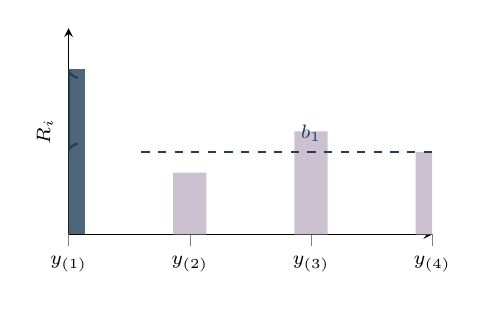
\begin{tikzpicture}
\begin{axis}[notes, width=6.2cm, height=4.2cm, ybar, bar width=12pt, ymin=0, ymax=1,
    xtick={1,...,4}, xticklabels={$y_{(1)}$,$y_{(2)}$,$y_{(3)}$,$y_{(4)}$}, ytick=\empty,
    ylabel={$R_i$}, ylabel style={font=\scriptsize}]
  \addplot[fill=AtlasCool!80, draw=none, bar shift=0pt] coordinates {(1,0.8)};
  \addplot[fill=AtlasSlate!35, draw=none, bar shift=0pt] coordinates {(2,0.3)(3,0.5)(4,0.4)};
  \draw[AtlasAccent, thick, dashed] (axis cs:1.6,0.4) -- (axis cs:4.4,0.4) node[pos=0.5, above, font=\scriptsize]{$b_1$};
  \draw[<->, AtlasCool, thick] (axis cs:1,0.4) -- node[left, font=\scriptsize]{$R_1-b_1$} (axis cs:1,0.8);
\end{axis}
\end{tikzpicture}\\
{\scriptsize $b_1$ = mean of the \textbf{other} samples.}
\end{minipage}\hfill
\begin{minipage}[c]{0.53\linewidth}
$k$ samples $y_{(i)}\sim\pi_\theta(\cdot\mid x)$, rewards $R_i=R(y_{(i)},x)$:
\begin{eqbox}
\begin{gather*}
  \frac1k\sum_{i=1}^k\Big[R_i-\underbrace{\frac{1}{k-1}\sum_{j\ne i}R_j}_{b_i}\Big]\nabla\log\pi_\theta(y_{(i)}\mid x)
\end{gather*}
\end{eqbox}
The baseline does not depend on $y_{(i)}$ $\Rightarrow$ \textbf{unbiased}: $\E[b_i\nabla\log\pi(y_{(i)})]=0$.
\end{minipage}

\begin{slatebox}[title={GRPO's mean vs.\ leave-one-out}]
GRPO's mean includes $y_{(i)}$ itself, but
\begin{gather*}
  R_i-\bar R = \tfrac{k-1}{k}\big(R_i-b_i\big),
\end{gather*}
the same up to scale. The real differences are the division by the \textbf{std} and the $1/|o_i|$ token average --- they reweight harder/easier questions and longer/shorter answers (cf.\ Liu et al., 2025, ``Understanding R1-Zero-Like Training'').
\end{slatebox}

\begin{keybox}[title={Results}]
RLOO ($k=4$) beats PPO's win rate by 10.3 (TL;DR), 14.5 (HH, Pythia) and 32.1 (HH, Llama) points --- with \textbf{three models, no critic}. It also beats RAFT (fine-tune on the best of $k$) at the same sampling budget, and DPO.
\end{keybox}

% ---------------------------------------------------------------------------
\section{Summary of Part V}
% ---------------------------------------------------------------------------

\subsection{What did we remove?}

\begin{center}
\small
\begin{tabular}{l c c c c c}
\toprule
 & {\color{AtlasWarm}\textbf{Reward model}} & {\color{AtlasWarm}\textbf{Critic}} & \textbf{KL to $\pi_{\mathrm{ref}}$} & \textbf{Samples of $\pi_\theta$} & \textbf{Clip} \\
\midrule
InstructGPT (PPO) & \cmark & \cmark & \cmark{} {\scriptsize in reward} & \cmark & \cmark \\
DPO & {\scriptsize implicit $\hat r_\theta$} & \xmark & \cmark{} {\scriptsize via $\beta$} & \xmark{} {\scriptsize offline} & \xmark \\
GRPO & \cmark & \xmark{} {\scriptsize group} & \cmark{} {\scriptsize in loss} & \cmark{} {\scriptsize $G$ per $q$} & \cmark \\
RLOO & \cmark & \xmark{} {\scriptsize leave-one-out} & \cmark{} {\scriptsize in reward} & \cmark{} {\scriptsize $k$ per $x$} & \xmark \\
\bottomrule
\end{tabular}
\end{center}

\begin{pair}
\begin{keybox}[title={Never removed: the KL to $\pi_{\mathrm{ref}}$}]
The learned reward is only trusted near $\pi^{SFT}$: InstructGPT adds the KL ``to mitigate over-optimization of the reward model''; DPO: it keeps the policy ``from deviating too far from the distribution on which the reward model is accurate''.
\end{keybox}
\begin{coolbox}[title={Why the critic could go}]
Many samples per prompt are cheap, and the prompt is the only real state.
\end{coolbox}
\end{pair}

\subsection{The thread: from CPI to LLMs}

\begin{center}
\footnotesize
\begin{tabularx}{\linewidth}{@{}>{\bfseries\raggedright\arraybackslash}p{2.5cm} L L L L@{}}
\toprule
 & \textbf{CPI} & \textbf{TRPO} & \textbf{PPO / GAE} & \textbf{LLMs} \\
\midrule
surrogate on old samples & policy advantage $\PA_{\pi,\mu}$ & $L_{\told}$ + importance weights & $L^{CPI}=\hat\E[r_t\hat A_t]$ & per-token ratio (GRPO) or plain REINFORCE \\
stay close & mixture step $\alpha$ & KL trust region $\delta$ & clip $\epsilon$ & KL to $\pi_{\mathrm{ref}}$ ($\beta$): \textbf{a new reason} \\
{\color{AtlasWarm}advantage / baseline} & $A_\pi$ from restarts & Monte Carlo $\hat Q$ & GAE$(\gamma,\lambda)$ with a critic & group mean / leave-one-out \\
where states come from & $D$, restarts $\mu$ & $\rho_0$ (vine: resets) & $\rho_0$ & prompts $x\sim D$ \\
\bottomrule
\end{tabularx}
\end{center}

\begin{enumerate}
  \item \textbf{Row 1}: PPO names its surrogate after CPI.
  \item \textbf{Row 2}: the \emph{reason} changes. In CPI/TRPO/PPO the step is small so the surrogate stays accurate; in RLHF the KL to $\pi_{\mathrm{ref}}$ keeps the policy where the learned reward model is accurate. The old/new-policy closeness is often barely active (RLOO: clipped $<5\%$).
  \item \textbf{Row 3}: the same bias--variance question, answered with less and less machinery as samples per prompt get cheap.
  \item \textbf{Row 4}: the start distribution $D$ of Part~I is the prompt distribution; deterministic, known dynamics would even allow CPI-style restarts.
\end{enumerate}


\clearpage
\appendix
% ===========================================================================
%  APPENDIX --- proofs, tools and side comparisons (the decks' backup slides)
% ===========================================================================
\part*{Appendix}
\addcontentsline{toc}{part}{Appendix}

\partintro{Proofs, tools and side comparisons. Each appendix is self-contained and is referenced from the main text.}

% ---------------------------------------------------------------------------
\section{Proof: the policy advantage is the derivative at $\alpha=0$}
\label{app:proof-pa}
% ---------------------------------------------------------------------------

\textbf{Claim} (K\&L Sec.~4.1, Eq.~4.2): $\left.\frac{\partial\eta_\mu}{\partial\alpha}\right|_{\alpha=0}=\frac{1}{1-\gamma}\PA_{\pi,\mu}(\pi')$.

\textbf{Step 1 --- the mixtures are a one-parameter policy class.}
\begin{gather*}
  \pi_\alpha(a;s) = (1-\alpha)\,\pi(a;s) + \alpha\,\pi'(a;s)
  \quad\Longrightarrow\quad
  \frac{\partial\pi_\alpha(a;s)}{\partial\alpha} = \pi'(a;s) - \pi(a;s)
\end{gather*}

\textbf{Step 2 --- the policy gradient theorem holds for \emph{any} parameter, so take $\theta:=\alpha$.}

\begin{pair}
\begin{coolbox}[title={Policy gradient, any $\theta\in\mathbb R^m$}]
\begin{gather*}
  \nabla_\theta\,\eta_\mu = \frac{1}{1-\gamma}\sum_s d_{\pi_\theta,\mu}(s)\sum_a \nabla_\theta\pi_\theta(a;s)\,Q_{\pi_\theta}(s,a)
\end{gather*}
\end{coolbox}
\begin{warmbox}[title={Mixture, at $\alpha=0$ ($\pi_0=\pi$)}]
\begin{gather*}
  \left.\frac{\partial\eta_\mu}{\partial\alpha}\right|_{0} = \frac{1}{1-\gamma}\,\E_{s\sim d_{\pi,\mu}}\Big[\textstyle\sum_a \big(\pi'-\pi\big)(a;s)\,Q_\pi(s,a)\Big]
\end{gather*}
\end{warmbox}
\end{pair}

\textbf{Step 3 --- turn $Q_\pi$ into $A_\pi$.} Since $\sum_a\pi(a;s)Q_\pi(s,a)=V_\pi(s)$ and $\sum_a\pi'(a;s)=1$:
\begin{gather*}
  \sum_a \pi'(a;s)\,Q_\pi(s,a) - V_\pi(s) = \sum_a\pi'(a;s)\big(Q_\pi(s,a)-V_\pi(s)\big) = \E_{a\sim\pi'(\cdot;s)}\big[A_\pi(s,a)\big]
\end{gather*}
\begin{eqbox}
\begin{gather*}
  \left.\frac{\partial\eta_\mu}{\partial\alpha}\right|_{\alpha=0}
  = \frac{1}{1-\gamma}\,\E_{s\sim d_{\pi,\mu}}\Big[\E_{a\sim\pi'(\cdot;s)}\big[A_\pi(s,a)\big]\Big]
  = \frac{1}{1-\gamma}\,\PA_{\pi,\mu}(\pi') \qquad \square
\end{gather*}
\end{eqbox}
{\small The factor $\frac{1}{1-\gamma}$ comes from our normalization: $d_{\pi,\mu}$ sums to 1 and $Q_\pi$ carries a $(1-\gamma)$.}

\subsection*{$\alpha$ and $\theta$ play the same role}

\begin{center}
\small
\begin{tabular}{l l l}
\toprule
 & {\color{AtlasWarm}\textbf{CPI: parameter $\alpha\in[0,1]$}} & {\color{AtlasCool}\textbf{TRPO: parameter $\theta\in\mathbb R^m$}} \\
\midrule
first order & $\eta_\mu(\pi_\alpha)=\eta_\mu(\pi)+\frac{\alpha}{1-\gamma}\PA_{\pi,\mu}(\pi')+O(\alpha^2)$ & $\eta(\pi_\theta)=L_{\pi_{\theta_0}}(\pi_\theta)+o(\|\theta-\theta_0\|)$ \\
source & this proof & TRPO Eq.~4 \\
step size & $\alpha$ itself & $\alpha=\DTV^{\max}(\piold,\pinew)$ (Thm.~1) \\
\bottomrule
\end{tabular}
\end{center}

\begin{keybox}
The proof never used that $\alpha$ is a mixing weight --- only that it parameterizes the policy. In a mixture, $\alpha$ is \textbf{both} the parameter and the distance (two mixtures differing by $\alpha$ disagree w.p.\ at most $\alpha$). For a general $\pi_\theta$ these are different things --- which is why TRPO needs $\DTV$, then KL.
\end{keybox}

% ---------------------------------------------------------------------------
\section{Comparing with Bertsekas \& Tsitsiklis}
\label{app:bt}
% ---------------------------------------------------------------------------

Our comparison (not in the paper), in five steps. Notation: $\bar A$ as in Lemma 6.1, $\Delta\eta=\eta_\mu(\pi')-\eta_\mu(\pi)$, and $(T_{\pi'}V)(s)=\E_{a\sim\pi'}\big[(1-\gamma)\mathcal R(s,a)+\gamma\,\E_{s'}V(s')\big]$, so that $\bar A=T_{\pi'}V_\pi-V_\pi$.

\subsection*{B.1 \ The B\&T bound: a worst case at every state}

Given $\varepsilon=\max_s|\tilde V(s)-V_\pi(s)|$ and $\pi'$ greedy for $\tilde V$ (i.e.\ $T_{\pi'}\tilde V\ge T_\pi\tilde V$):
\begin{gather*}
  \begin{aligned}
    T_{\pi'}V_\pi \;&\ge\; T_{\pi'}\tilde V - \gamma\varepsilon && \text{\small\color{NoteGray}$V_\pi$ vs.\ $\tilde V$ at the next state: error $\le\varepsilon$, times $\gamma$}\\
    &\ge\; T_{\pi}\tilde V - \gamma\varepsilon && \text{\small\color{NoteGray}$\pi'$ is greedy for $\tilde V$}\\
    &\ge\; T_\pi V_\pi - 2\gamma\varepsilon \;=\; V_\pi - 2\gamma\varepsilon && \text{\small\color{NoteGray}the same error again}
  \end{aligned}
\end{gather*}
\begin{eqbox}
\begin{gather*}
  \bar A(s) \;\ge\; -2\gamma\varepsilon \ \ \text{at \textbf{every} } s
  \quad\Longrightarrow\quad
  \Delta\eta = \frac{1}{1-\gamma}\,\E_{d_{\pi',\mu}}\big[\bar A\big] \;\ge\; -\frac{2\gamma\varepsilon}{1-\gamma}
\end{gather*}
\end{eqbox}
\begin{warnbox}[title={Only a floor}]
$\varepsilon$ is \textbf{how wrong our values are}. It only limits how \textbf{negative} $\bar A$ can be; nothing positive is known, since $\pi'$ is greedy for the \emph{wrong} values. ($\varepsilon=0$: $\bar A\ge0$ everywhere --- exact policy improvement.) Because the floor holds at every state, we never need $d_{\pi',\mu}$.
\end{warnbox}

\subsection*{B.2 \ Theorem 4.1 at $\alpha=1$}

Split the new states into old states + shift:
\begin{gather*}
  (1-\gamma)\Delta\eta = \textstyle\sum_s d_{\pi',\mu}(s)\,\bar A(s)
  = \underbrace{\textstyle\sum_s d_{\pi,\mu}(s)\,\bar A(s)}_{=\,\PA\ \text{(measurable)}}
  + \underbrace{\textstyle\sum_s \big(d_{\pi',\mu}-d_{\pi,\mu}\big)(s)\,\bar A(s)}_{\text{shift}}
\end{gather*}
\begin{enumerate}
  \item Shift $\ge -\|d_{\pi',\mu}-d_{\pi,\mu}\|_1\cdot\varepsilon$, with $\varepsilon=\max_s|\bar A(s)|=\max_s|\E_{a\sim\pi'}A_\pi(s,a)|$. It needs $|\cdot|$: the shift can also move mass \emph{away} from states where $\bar A>0$.
  \item Same start $\mu$ $\Rightarrow$ only $t\ge1$ can differ: \ $\|d_{\pi',\mu}-d_{\pi,\mu}\|_1\le(1-\gamma)\sum_{t\ge1}\gamma^t\cdot2=2\gamma$.
\end{enumerate}
\begin{eqbox}
\begin{gather*}
  \Delta\eta \;\ge\; \frac{\PA}{1-\gamma} - \frac{2\gamma\varepsilon}{1-\gamma} \qquad \text{= Thm 4.1 at $\alpha=1$}
\end{gather*}
\end{eqbox}
{\small The new ingredient is $\PA$: B\&T never measure any average of the true $\bar A$. The $2\gamma$ is the same number as in B\&T, from a different place: there, two estimation errors one step ahead; here, two state distributions that agree at the start.}

\subsection*{B.3 \ Why the mixture helps}

Same split for $\pinew=(1-\alpha)\pi+\alpha\pi'$:
\begin{enumerate}
  \item \textbf{Per state}: $\bar A_{\mathrm{new}}(s)=\alpha\bar A(s)$ $\Rightarrow$ gain $\alpha\PA$, \ $\max_s|\bar A_{\mathrm{new}}|=\alpha\varepsilon$.
  \item \textbf{Shift}: $\pinew$ acts like $\pi$ w.p.\ $1-\alpha$ each step, so $\Pr(\text{deviated by }t)\le1-(1-\alpha)^t$, and
  \begin{gather*}
    \|d_{\pinew,\mu}-d_{\pi,\mu}\|_1 \le (1-\gamma)\textstyle\sum_t\gamma^t\,2\big(1-(1-\alpha)^t\big) = \frac{2\alpha\gamma}{1-\gamma(1-\alpha)}
  \end{gather*}
  \item \textbf{Multiply}: $(1-\gamma)\Delta\eta \ge \alpha\PA - \alpha\varepsilon\cdot\frac{2\alpha\gamma}{1-\gamma(1-\alpha)}$ \ = Thm 4.1.
\end{enumerate}
\begin{keybox}
Both factors of the penalty carry an $\alpha$ $\Rightarrow$ $\alpha^2$. Small $\alpha$: the gain wins. $\alpha=1$: since $\PA\le\varepsilon$ we would need $\PA>2\gamma\varepsilon$ --- impossible for $\gamma\ge\frac12$. The positive term alone does not justify the full greedy step; \textbf{the small step does}.
\end{keybox}

\subsection*{B.4 \ Same penalty, different $\varepsilon$}

\begin{center}
\small
\begin{tabular}{l l l l}
\toprule
 & {\color{AtlasWarm}\textbf{B\&T}} & {\color{AtlasCool}\textbf{K\&L, Thm 4.1}} & \textbf{TRPO, Thm 1} \\
\midrule
$\varepsilon=$ & $\max_s|\tilde V(s)-V_\pi(s)|$ & $\max_s|\E_{a\sim\pi'}A_\pi(s,a)|$ & $\max_{s,a}|A_\pi(s,a)|$ \\
depends on & our estimate $\tilde V$ & the pair $\pi,\pi'$ & $\pi$ only \\
measures & how wrong our values are & largest one-step gain/loss of $\pi'$ & scale of the advantages \\
step size & fixed: full greedy step & $\alpha$ (mixture weight) & $\alpha=\DTV^{\max}(\pi,\tilde\pi)$ \\
\bottomrule
\end{tabular}
\end{center}
\begin{itemize}
  \item \textbf{Common}: the price of not knowing $\bar A$ on the states the new policy visits.
  \item \textbf{Why it changed}: in B\&T, $\pi'$ is fixed by $\tilde V$, so only the estimate can go wrong. K\&L ask \emph{how far may we step?} --- so $\varepsilon$ measures the step, not the estimate. It cannot be estimated either (a max over all states), so Cor.~4.2 replaces it by $R$.
\end{itemize}

\subsection*{B.5 \ Where the error went, and what TRPO does}

\textbf{Where did B\&T's approximation error go?} Not into Thm 4.1's $\varepsilon$, but into
\begin{enumerate}
  \item the estimate of $\PA$ from $\mu$-restarts (sampling error, Hoeffding);
  \item the accuracy of the greedy chooser $G_\varepsilon$.
\end{enumerate}
Both are \textbf{averages} under $d_{\pi,\mu}$ --- much weaker than B\&T's $\max_s$. (The $\varepsilon$ of $G_\varepsilon$ and Thm 4.4 is the chooser's accuracy, not the $\varepsilon$ of Thm 4.1.)

\textbf{TRPO splits K\&L's $\varepsilon$} into a step and a scale (TRPO App.~A, Lemma 2: couple $a\sim\pi$, $\tilde a\sim\tilde\pi$ to disagree w.p.\ at most $\alpha$; use $\E_{a\sim\pi}A_\pi=0$):
\begin{eqbox}
\begin{gather*}
  |\bar A(s)| \;\le\; 2\,\underbrace{\DTV\big(\pi(\cdot|s),\tilde\pi(\cdot|s)\big)}_{\text{policy change}\ \le\ \alpha}\cdot\underbrace{\max_{s,a}|A_\pi(s,a)|}_{\text{advantage scale}}
\end{gather*}
\end{eqbox}
\begin{keybox}
The step becomes a \textbf{distance between policies} that the algorithm controls $\Rightarrow$ trust region. Plugging this into the K\&L argument gives the $\frac{4\epsilon\gamma}{(1-\gamma)^2}\alpha^2$ penalty, with $4=2\cdot2$.
\end{keybox}

% ---------------------------------------------------------------------------
\section{From $\E_{s\sim d}$ to a sum over time}
\label{app:sumswap}
% ---------------------------------------------------------------------------

The second equality of Lemma 6.1, in four steps:
\begin{gather*}
  \begin{aligned}
    \frac{1}{1-\gamma}\E_{s\sim d_{\pi',\mu}}[\bar A(s)] &= \frac{1}{1-\gamma}\textstyle\sum_s d_{\pi',\mu}(s)\,\bar A(s) && \text{\small\color{NoteGray}1. expectation = weighted sum}\\
    &= \textstyle\sum_s \Big[\sum_t \gamma^t \Pr(s_t{=}s)\Big]\bar A(s) && \text{\small\color{NoteGray}2. definition of $d$; $(1-\gamma)$ cancels}\\
    &= \textstyle\sum_t \gamma^t \Big[\sum_s \Pr(s_t{=}s)\,\bar A(s)\Big] && \text{\small\color{NoteGray}3. swap the sums}\\
    &= \textstyle\sum_t \gamma^t\, \E\big[\bar A(s_t)\big] = \E\Big[\sum_t \gamma^t \bar A(s_t)\Big] && \text{\small\color{NoteGray}4. definition of $\E$; linearity}
  \end{aligned}
\end{gather*}

\begin{minipage}[c]{0.45\linewidth}
\centering
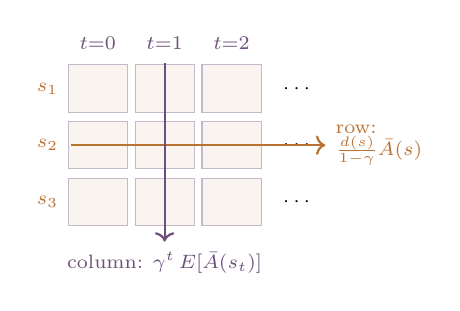
\begin{tikzpicture}[x=0.85cm, y=0.72cm, font=\scriptsize]
  \foreach \s/\y in {1/0, 2/-1, 3/-2} {
    \node[AtlasWarm] at (-0.75,\y) {$s_\s$};
    \foreach \t in {0,1,2} \node[draw=AtlasSlate!40, minimum width=0.75cm, minimum height=0.6cm, fill=AtlasWarm!8] at (\t,\y) {};
    \node at (3,\y) {$\cdots$};}
  \foreach \t in {0,1,2} \node[AtlasSlate] at (\t,0.8) {$t{=}\t$};
  \draw[AtlasWarm, thick, ->] (-0.4,-1) -- (3.4,-1) node[right, align=left]{row:\\ $\frac{d(s)}{1-\gamma}\bar A(s)$};
  \draw[AtlasSlate, thick, ->] (1,0.45) -- (1,-2.7) node[below]{column: $\gamma^t\,\E[\bar A(s_t)]$};
\end{tikzpicture}
\end{minipage}\hfill
\begin{minipage}[c]{0.52\linewidth}
\begin{itemize}
  \item \textbf{Cell} $(s,t)$: $\gamma^t\Pr(s_t{=}s)\,\bar A(s)$.
  \item Sum by \textcolor{AtlasWarm}{\textbf{rows}} (step 2) or by \textcolor{AtlasSlate}{\textbf{columns}} (step 3): same total.
  \item The swap is allowed: $|\text{cell}|\le\gamma^t\Pr(s_t{=}s)R$, and these sum to $R/(1-\gamma)<\infty$ (absolute convergence).
\end{itemize}
\end{minipage}

\begin{notebox}
$\E[\bar A(s_t)]$ is over $s_t\sim p_t$, $p_t(s)=\Pr(s_t{=}s\mid s_0\sim\mu,\pi')$ --- the state at time $t$, \textbf{not discounted}; one distribution per $t$. $\E[\sum_t\cdots]$ is over trajectories $s_0\sim\mu$, $a_t\sim\pi'$, $s_{t+1}\sim P$. The discount sits only in the weights $\gamma^t$.
\end{notebox}

% ---------------------------------------------------------------------------
\section{The Gibbs (softmax) policy}
\label{app:gibbs}
% ---------------------------------------------------------------------------

\begin{minipage}[c]{0.44\linewidth}
\centering
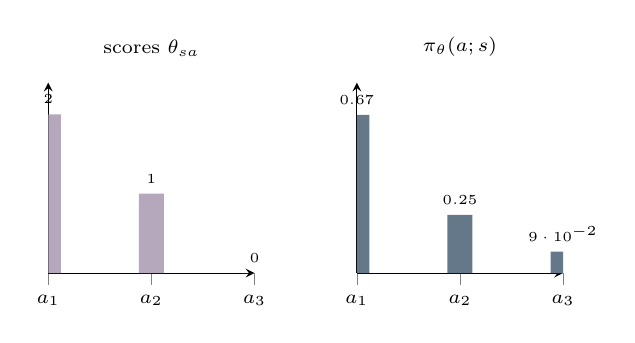
\begin{tikzpicture}
\begin{axis}[notes, name=sc, width=4.2cm, height=4cm, ybar, bar width=9pt, ymin=0, ymax=2.4,
    xtick={1,2,3}, xticklabels={$a_1$,$a_2$,$a_3$}, ytick=\empty, title={\scriptsize scores $\theta_{sa}$},
    nodes near coords, nodes near coords style={font=\tiny}]
  \addplot[fill=AtlasSlate!50, draw=none] coordinates {(1,2)(2,1)(3,0)};
\end{axis}
\begin{axis}[notes, at={(sc.east)}, anchor=west, xshift=1.3cm, width=4.2cm, height=4cm, ybar, bar width=9pt, ymin=0, ymax=0.8,
    xtick={1,2,3}, xticklabels={$a_1$,$a_2$,$a_3$}, ytick=\empty, title={\scriptsize $\pi_\theta(a;s)$},
    nodes near coords, nodes near coords style={font=\tiny}]
  \addplot[fill=AtlasCool!70, draw=none] coordinates {(1,0.665)(2,0.245)(3,0.090)};
\end{axis}
\end{tikzpicture}\\
{\scriptsize One state, three actions. Every action keeps \textbf{some} probability.}
\end{minipage}\hfill
\begin{minipage}[c]{0.53\linewidth}
One parameter per state--action pair (``table lookup''):
\begin{eqbox}
\begin{gather*}
  \pi_\theta(a;s) = \frac{e^{\theta_{sa}}}{\sum_b e^{\theta_{sb}}}
\end{gather*}
\end{eqbox}
\end{minipage}

\begin{enumerate}
  \item \textbf{Why ``Gibbs''}: the Boltzmann distribution of physics, $p\propto e^{-E/T}$, with $\theta=-E/T$. A temperature ($\theta/T$): $T\to0$ gives argmax, $T\to\infty$ uniform.
  \item \textbf{Always stochastic}: $\pi_\theta(a;s)>0$; deterministic only as $\theta\to\pm\infty$.
  \item \textbf{Rich}: any policy with full support, in every state independently. So the trouble in Example~2 comes from the \emph{gradient}, not from the class.
  \item \textbf{Not unique}: adding a constant to all $\theta_{sa}$ of one state leaves $\pi$ unchanged.
  \item \textbf{Simple score} (derivation below): $\partial_{\theta_{sb}}\log\pi_\theta(a;s)=\mathbf 1[a=b]-\pi_\theta(b;s)$.
\end{enumerate}

\subsection*{Deriving the score}

One state, so drop $s$ ($\theta_a=\theta_{sa}$):
\begin{gather*}
  \pi(a) = \frac{e^{\theta_a}}{\sum_c e^{\theta_c}}
  \quad\Longrightarrow\quad
  \log\pi(a) = \theta_a - \log\textstyle\sum_c e^{\theta_c}
  \quad\Longrightarrow\quad
  \partial_{\theta_b}\log\pi(a) = \underbrace{\partial_{\theta_b}\theta_a}_{\mathbf 1[a=b]} - \underbrace{\frac{e^{\theta_b}}{\sum_c e^{\theta_c}}}_{\pi(b)}
\end{gather*}

\begin{itemize}
  \item \textbf{Vector form}: $\nabla_{\theta_s}\log\pi(a;s)=e_a-\pi(\cdot\,;s)$ --- ``the action taken minus the average action''. Other states get derivative 0.
  \item \textbf{Check}: $\E_{a\sim\pi}\big[\mathbf 1[a=b]-\pi(b)\big]=0$ --- the identity $\E[\nabla\log\pi]=0$ that makes baselines unbiased.
  \item \textbf{In REINFORCE}: taking $a_t$ with $\hat Q_t>0$ raises $\theta_{sa_t}$ by $\alpha\hat Q_t(1-\pi(a_t;s))$ and lowers each other $\theta_{sb}$ by $\alpha\hat Q_t\pi(b;s)$. Only visited states get gradient --- why a rarely visited state $j$ learns slowly.
  \item Two actions: $\pi(a_1)=\sigma(\theta_1-\theta_2)$ and $(\log\sigma)'=1-\sigma$.
\end{itemize}

% ---------------------------------------------------------------------------
\section{Why the log-derivative trick is unbiased}
\label{app:logderiv}
% ---------------------------------------------------------------------------

$\theta$ sits in the \textbf{sampling distribution}, not in $R(\tau)$, so averaging $\nabla_\theta R$ gives nothing. The trajectory density:
\begin{gather*}
  p_\theta(\tau) = {\color{NoteGray}D(s_0)}\prod_t {\color{AtlasCool}\pi_\theta(a_t;s_t)}\,{\color{NoteGray}P(s_{t+1};s_t,a_t)}
\end{gather*}

\begin{enumerate}
  \item Use $\nabla p=p\,\nabla\log p$ wherever $p>0$:
  \begin{gather*}
    \nabla_\theta\,\eta_D = \sum_\tau \nabla_\theta\, p_\theta(\tau)\, R(\tau) = \E_{\tau\sim\pi_\theta}\big[R(\tau)\,\nabla_\theta\log p_\theta(\tau)\big]
  \end{gather*}
  \item The log turns $\prod$ into $\sum$, and the grey terms have no $\theta$:
  \begin{gather*}
    \nabla_\theta\log p_\theta(\tau) = \textstyle\sum_t \nabla_\theta\log{\color{AtlasCool}\pi_\theta(a_t;s_t)}
  \end{gather*}
\end{enumerate}

\begin{keybox}
$\hat g = R(\tau)\sum_t \nabla_\theta\log\pi_\theta(a_t;s_t)$, $\tau\sim\pi_\theta$ $\Rightarrow$ $\E[\hat g]=\nabla_\theta\eta_D$ \textbf{exactly}, and no need to know $P$.
\end{keybox}

\textbf{Unbiased is not low variance.} Two standard changes keep it unbiased and reduce the noise:
\begin{enumerate}
  \item Weight each $\nabla\log\pi_\theta(a_t;s_t)$ only by rewards \textbf{after} $t$ (an action cannot affect earlier rewards) --- the $\hat Q_t$ of REINFORCE.
  \item Subtract a \textbf{baseline} $b(s_t)$, since $\E_{a\sim\pi_\theta}[\nabla_\theta\log\pi_\theta(a;s)]=\sum_a\nabla_\theta\pi_\theta(a;s)=\nabla_\theta1=0$. With $b=V_\pi$ the weight becomes the advantage --- the road to GAE.
\end{enumerate}
{\small Williams (1992); also called the score-function or likelihood-ratio estimator. $R(\tau)=(1-\gamma)\sum_t\gamma^tr_t$.}

% ---------------------------------------------------------------------------
\section{CPI through the SGD lens}
\label{app:cpi-sgd}
% ---------------------------------------------------------------------------

Take the table $\pi(a;s)$ itself as the parameter: CPI is a \textbf{first-order method} on $\eta_\mu$.

\begin{center}
\footnotesize
\begin{tabularx}{\linewidth}{@{}r L L@{}}
\toprule
 & {\color{AtlasSlate}\textbf{SGD (non-convex, smooth)}} & {\color{AtlasWarm}\textbf{CPI}} \\
\midrule
{\color{NoteGray}direction} & $\hat g\approx\nabla J(w)$ & greedy $\pi'=G_\varepsilon(\pi,\mu)$: best linearized direction \\
{\color{NoteGray}step} & $w\leftarrow w+a_k\hat g$ & $\pi\leftarrow(1-\alpha)\pi+\alpha\pi'$ (Frank--Wolfe step) \\
{\color{NoteGray}step size} & $\sum_ka_k=\infty$, $\sum_ka_k^2<\infty$ & $\alpha\propto\hat\PA$: slope over a smoothness bound \\
{\color{NoteGray}noise} & averages out over many steps & each step accurate w.h.p.\ (Hoeffding) \\
{\color{NoteGray}stationary} & $\|\nabla J(w_R)\|\le\epsilon$, random iterate & $\OPT(\PA_{\pi,\mu})<2\varepsilon$, last iterate \\
{\color{NoteGray}cost} & $O(\sigma^2/\epsilon^4)$ samples & $72R^2/\varepsilon^2$ updates $\times$ $\tilde O(R^2/\varepsilon^2)$ rollouts \\
{\color{NoteGray}global?} & \xmark\ a stationary point can be bad & \cmark\ Thm.~6.2, up to the mismatch factor \\
\bottomrule
\end{tabularx}
\end{center}

\begin{enumerate}
  \item \textbf{CPI is Frank--Wolfe on the table $\pi(a;s)$.} $\partial\eta_\mu/\partial\pi(a;s)=d_{\pi,\mu}(s)Q_\pi(s,a)/(1-\gamma)$, so the slope toward $\pi'$ is $\langle\nabla\eta_\mu,\pi'-\pi\rangle=\PA_{\pi,\mu}(\pi')/(1-\gamma)$. $G_\varepsilon$ maximizes the linearization; per state the maximum is the greedy vertex $\arg\max_aA_\pi(s,a)$. $\OPT(\PA)/(1-\gamma)$ is the Frank--Wolfe gap. Caveat: $\eta_\mu$ is not concave in $\pi$. (Vieillard, Pietquin \& Geist 2019; Scherrer \& Geist 2014; Lacoste-Julien 2016.)
  \item \textbf{Gibbs parameterization.} $\partial\eta_\mu/\partial\theta_{sa}=d_{\pi,\mu}(s)\pi(a;s)A_\pi(s,a)/(1-\gamma)$: the same advantage, but times $\pi(a;s)$, so good unlikely actions and unvisited states barely move (Ex.~1--2). The natural gradient (Kakade 2001) drops both factors: $\pi_{\text{new}}\propto\pi\,e^{\beta A_\pi}$, a soft move toward greedy. CPI's mixture is the hard version.
  \item \textbf{Link to SGD.} SGD lets unbiased noise cancel over many steps; CPI makes each step accurate to $\pm\varepsilon/3$ w.h.p.\ and steps only if $\hat\PA\ge2\varepsilon/3$: monotone improvement, a guarantee for the last iterate. Counting (gain $\ge\varepsilon^2/72R$, $\eta_\mu\le R$) is the descent-lemma argument. Thm.~6.2 is what later theory calls \textbf{gradient domination} (Agarwal, Kakade, Lee \& Mahajan 2021).
\end{enumerate}

% ---------------------------------------------------------------------------
\section{Building $G_\varepsilon$ by regression on advantages}
\label{app:greedy}
% ---------------------------------------------------------------------------

\begin{center}
\begin{tikzpicture}[>=Stealth, box/.style={fl, cbox=AtlasCool, font=\scriptsize, minimum height=1.0cm, text width=3.1cm}]
  \node[box] (data) at (0,0) {\textbf{Data} from $\mu$-restarts\\$s\sim d_{\pi,\mu}$, $a$ uniform,\\rollout $\hat Q_\pi(s,a)$};
  \node[box] (fit) at (4.2,0) {\textbf{Regression}\\$f_\pi(s,a)\approx A_\pi(s,a)$};
  \node[box, cbox=AtlasWarm] (pol) at (8.4,0) {\textbf{Greedy in $f_\pi$}\\$\pi'(s)=\arg\max_a f_\pi(s,a)$};
  \draw[->, thick, AtlasSlate] (data) -- (fit);
  \draw[->, thick, AtlasSlate] (fit) -- (pol);
\end{tikzpicture}
\end{center}

\begin{defbox}{required accuracy (K\&L Sec.~7.1)}
\begin{gather*}
  L(f_\pi) = \underbrace{\E_{s\sim d_{\pi,\mu}}}_{\text{average over states}}\ \underbrace{\max_a}_{\text{worst action}}\big|A_\pi(s,a)-f_\pi(s,a)\big| \;\le\; \frac{\varepsilon}{2}
\end{gather*}
\end{defbox}

\textbf{Why it suffices.} With $e(s)=\max_a|A_\pi-f_\pi|$, $\hat a=\arg\max_af_\pi$, $a^*=\arg\max_aA_\pi$:
\begin{gather*}
  A_\pi(s,\hat a) \ge f_\pi(s,\hat a)-e(s) \ge f_\pi(s,a^*)-e(s) \ge A_\pi(s,a^*)-2e(s) \\
  \E_{s\sim d_{\pi,\mu}}:\quad \PA_{\pi,\mu}(\pi') \ge \OPT(\PA_{\pi,\mu}) - 2L \ge \OPT(\PA_{\pi,\mu}) - \varepsilon
\end{gather*}

\begin{keybox}
An \textbf{average} ($\ell_1$) error over $d_{\pi,\mu}$, not the $\max_s$ ($\ell_\infty$) error of greedy DP (Gap 1): rarely visited states may be fit badly.
\end{keybox}

\begin{itemize}
  \item \textbf{Fitting $Q$ is enough}: $A_\pi=Q_\pi-V_\pi(s)$ shifts each state by a constant --- same error, same argmax.
  \item \textbf{Link to usual losses}: $\max_a|e|\le n_a\E_{a\sim\text{unif}}|e|\le n_a\sqrt{\E e^2}$, so an MSE below $(\varepsilon/(2n_a))^2$ suffices (pessimistic).
  \item The paper does not bound the samples this regression needs, so the total cost of CPI is open. Descendants: API with classifiers (Lagoudakis \& Parr 2003).
\end{itemize}

% ---------------------------------------------------------------------------
\section{Stopping with probability $1-\gamma$ samples $d_{\pi,\mu}$}
\label{app:geom}
% ---------------------------------------------------------------------------

Run $\pi$ from $s_0\sim\mu$; after each step stop w.p.\ $1-\gamma$, independently of the trajectory. Return $s_\tau$.

\begin{minipage}[c]{0.52\linewidth}
\begin{enumerate}
  \item $\Pr(\tau=t)=\gamma^t(1-\gamma)$ \ ($t$ continues, then one stop).
  \item $\Pr(s_\tau=s)=\sum_t\Pr(\tau=t)\Pr(s_t=s)$ \ (needs independence).
  \item $=(1-\gamma)\sum_t\gamma^t\Pr(s_t=s\mid\pi,\mu)=d_{\pi,\mu}(s)$.
\end{enumerate}
\end{minipage}\hfill
\begin{minipage}[c]{0.45\linewidth}
\centering
\begin{tikzpicture}
\begin{axis}[notes, width=6.4cm, height=4cm, ybar, bar width=6pt, ymin=0, ymax=0.33,
    xtick={0,2,...,10}, ytick={0,0.1,0.2,0.3}, xlabel={$t$}, title={\small $\Pr(\tau=t)=(1-\gamma)\gamma^t$, \ $\gamma=0.7$}]
  \addplot[fill=AtlasWarm!70, draw=none, domain=0:10, samples=11] {0.3*0.7^x};
\end{axis}
\end{tikzpicture}
\end{minipage}

\begin{keybox}
The discount weights $(1-\gamma)\gamma^t$ are a \textbf{geometric distribution} over $t$. $\gamma$ = probability of surviving one more step; $d_{\pi,\mu}$ = the distribution of the state where an episode of random length ends. The $(1-\gamma)$ in $d_{\pi,\mu}$ is what makes $\sum_t\Pr(\tau=t)=1$.
\end{keybox}
{\small Cost of one sample: $\E[\tau]=\gamma/(1-\gamma)$, about 99 steps at $\gamma=0.99$.}

% ---------------------------------------------------------------------------
\section{Hoeffding's inequality and the estimate of $\PA$}
\label{app:hoeffding}
% ---------------------------------------------------------------------------

\begin{thmbox}{Hoeffding (1963)}
If $X_1,\dots,X_k$ are \textbf{independent} and $X_i\in[a,b]$ a.s., then for $\bar X=\frac1k\sum_iX_i$:
\begin{gather*}
  \Pr\big(|\bar X-\E\bar X|>\Delta\big) \;\le\; 2\exp\!\Big(-\frac{2k\Delta^2}{(b-a)^2}\Big)
\end{gather*}
\end{thmbox}

\textbf{Conditions for the $x_i$ of CPI:}
\begin{enumerate}
  \item \textbf{Independent}: each $x_i$ comes from a fresh $\mu$-restart.
  \item \textbf{Bounded}: $\hat Q_i\in[0,R]$, $|\pi'-\pi|\le1$ $\Rightarrow$ $x_i\in[-n_aR,n_aR]$, $b-a=2n_aR$.
  \item \textbf{Right mean}: $\E x_i=\PA$ (uniform $a$, weight $n_a$); the bias of a finite rollout is kept below $\varepsilon/6$.
\end{enumerate}

\begin{eqbox}
\begin{gather*}
  \Pr\big(|\hat\PA-\PA|>\Delta\big) \le 2e^{-k\Delta^2/(2n_a^2R^2)}
  \quad\Longrightarrow\quad
  k \ge \frac{2n_a^2R^2}{\Delta^2}\log\frac2\delta \ \text{ gives error } \le\Delta \text{ w.p.\ } \ge1-\delta
\end{gather*}
\end{eqbox}

\begin{notebox}
No identical distribution is needed, and no variance enters --- the bound is loose when the $x_i$ rarely reach the ends of the range. The range $2n_aR$ is what costs: the importance weight $n_a$ widens it, hence $k\propto n_a^2$. In CPI, $\Delta=\varepsilon/3$ and $\delta$ is split over at most $72R^2/\varepsilon^2$ updates (union bound), which gives the $O\big(\frac{R^2}{\varepsilon^2}\log\frac{R^2}{\delta\varepsilon^2}\big)$ restarts per update (the paper drops $n_a$).
\end{notebox}

% ---------------------------------------------------------------------------
\section{Importance sampling in CPI, and why uniform actions}
\label{app:is-cpi}
% ---------------------------------------------------------------------------

The estimate of $\PA$ needs a \textbf{sum} over actions, but each rollout tries \textbf{one} action.

\begin{minipage}[c]{0.54\linewidth}
\begin{enumerate}
  \item \textbf{Sample from $q$, reweight by $w=p/q$} (needs $q>0$ where $p>0$):
  \begin{gather*}
    \E_{a\sim p}[f] = \textstyle\sum_a q\,\frac{p}{q}\,f = \E_{a\sim q}\big[w\,f\big]
  \end{gather*}
  \item \textbf{A plain sum is the case $p\equiv1$}; CPI takes $q$ uniform:
  \begin{gather*}
    \textstyle\sum_a f(a) = \E_{a\sim q}\Big[\frac{f(a)}{q(a)}\Big] = \E_{a\sim\text{unif}}\big[n_a f(a)\big]
  \end{gather*}
  \item \textbf{Unbiased, but the weight stretches the range}: $|f|\le R\Rightarrow|n_af|\le n_aR\Rightarrow n_a^2$ in Hoeffding.
\end{enumerate}
\end{minipage}\hfill
\begin{minipage}[c]{0.43\linewidth}
\centering
\begin{tikzpicture}
\begin{axis}[notes, width=6.4cm, height=4.6cm, ybar, bar width=7pt, ymin=-1.5, ymax=4,
    xtick={1,...,4}, xticklabels={$a_1$,$a_2$,$a_3$,$a_4$}, ytick={0,1.4}, axis x line=middle,
    legend style={at={(0.5,1.03)}, anchor=south, legend columns=2}, area legend]
  \addplot[fill=AtlasCool!70, draw=none] coordinates {(1,0.6)(2,-0.3)(3,0.9)(4,0.2)};
  \addlegendentry{$f(a)$}
  \addplot[fill=AtlasWarm!70, draw=none] coordinates {(1,2.4)(2,-1.2)(3,3.6)(4,0.8)};
  \addlegendentry{$n_af(a)$}
  \draw[AtlasWarm, thick, dashed] (axis cs:0.5,1.4) -- (axis cs:4.5,1.4);
\end{axis}
\end{tikzpicture}\\
{\scriptsize Four actions, $\sum_af=1.4$; the orange values average to $1.4$.}
\end{minipage}

\subsection*{Why uniform? Two ways to sample the same target}

At a state $s\sim d_{\pi,\mu}$:
\begin{gather*}
  \textstyle\sum_a\big(\pi'-\pi\big)(a;s)\,Q_\pi(s,a)
  \;=\; \underbrace{\E_{a\sim\text{unif}}\big[n_a(\pi'-\pi)(a;s)\,Q_\pi(s,a)\big]}_{\text{importance sampling, }p\equiv1}
  \;=\; \underbrace{\E_{a\sim\pi'}\big[Q_\pi(s,a)\big]-V_\pi(s)}_{\text{sample from }\pi'}
\end{gather*}

\begin{pair}
\begin{coolbox}[title={CPI: $a$ uniform, one rollout of $\pi$}]
\small $x=n_a(\pi'-\pi)(a;s)\,\hat Q(s,a)\in[-n_aR,n_aR]$
\begin{itemize}
  \item[$+$] same data as $G_\varepsilon$ (needs $\hat Q$ for \emph{every} $a$)
  \item[$+$] one batch scores \emph{any} candidate $\pi'$
  \item[$-$] factor $n_a^2$ in the sample count
\end{itemize}
\end{coolbox}
\begin{slatebox}[title={Alternative: $a\sim\pi'$, rollouts of $\pi$}]
\small $x=\hat Q(s,a)-\hat V(s)\in[-R,R]$
\begin{itemize}
  \item[$+$] no $n_a$; still only rollouts of $\pi$ (Q2 holds)
  \item[$-$] needs $\pi'$ \emph{before} sampling
  \item[$-$] a second estimate per state ($\hat V$)
\end{itemize}
\end{slatebox}
\end{pair}

\begin{warnbox}[title={Not plain IS with $q=\pi'$}]
The weight would be $1/\pi'(a)$, but a greedy $\pi'$ is often deterministic, so $\pi'(a)=0$ where $\pi(a)Q_\pi(s,a)\neq0$ and the identity fails. The subtraction of $V_\pi$ in the second form is the same baseline idea that later appears as the advantage in TRPO/PPO.
\end{warnbox}

% ---------------------------------------------------------------------------
\section{TRPO with continuous states and actions}
\label{app:trpo-cont}
% ---------------------------------------------------------------------------

TRPO footnote~1: ``replace the sums with integrals''. \textbf{True} --- no proof uses finiteness. But ``integrals'' hides some conditions.

\begin{pair}
\begin{keybox}[title={Why it carries over}]
\begin{itemize}
  \item \textbf{Performance difference}: telescoping, any space.
  \item \textbf{Coupling}: mass $1-\DTV$ on $\{a=\tilde a\}$ --- also for densities (maximal coupling on standard Borel spaces).
  \item \textbf{Perturbation} (App.~B): matrices $\to$ Markov operators, same norms.
\end{itemize}
\end{keybox}
\begin{warnbox}[title={What ``integrals'' hides}]
\begin{enumerate}
  \item \textbf{Bounded} $\epsilon=\sup_{s,a}|A_\pi(s,a)|<\infty$.
  \item \textbf{max $\to$ sup} over \textbf{all} states, not just visited ones.
  \item \textbf{Stochastic} policies: deterministic $\Rightarrow\DKL=\infty$.
  \item \textbf{Measurable} kernels; $\rho_\pi$ is a measure.
\end{enumerate}
\end{warnbox}
\end{pair}

\begin{notebox}
Condition 1 is often \textbf{vacuous} in continuous control: Gaussian actions with reward $-\|u\|^2$ (their Swimmer: $r=v_x-10^{-5}\|u\|^2$) give $\epsilon=\infty$. The practical algorithm drops the bound anyway (mean KL, fixed $\delta$). For a Gaussian with fixed $\sigma$: $\DKL(s)=\|\mu_{\mathrm{new}}(s)-\mu_{\mathrm{old}}(s)\|^2/2\sigma^2$.
\end{notebox}

% ---------------------------------------------------------------------------
\section{One problem, several known algorithms}
\label{app:trpo-conn}
% ---------------------------------------------------------------------------

\begin{center}
\small
\begin{tabular}{l l l}
\toprule
\textbf{Objective} & \textbf{Constraint / penalty} & \textbf{Algorithm} \\
\midrule
linear in $\theta$ & $\frac12\|\theta-\told\|^2\le\delta$ & vanilla policy gradient \\
linear in $\theta$ & quadratic KL, fixed step $\frac1\lambda$ & natural policy gradient \\
full $L_{\piold}(\pi)$ & none & policy iteration \\
$L_{\told}(\theta)$ & $\bar D_{\mathrm{KL}}\le\delta$, enforced & \textbf{TRPO} \\
\bottomrule
\end{tabular}
\end{center}

\begin{itemize}
  \item \textbf{NPG vs.\ TRPO}: the same direction $A^{-1}g$; TRPO \textbf{enforces} the KL constraint at each step --- this matters on larger problems.
  \item \textbf{Related}: REPS constrains the joint $p(s,a)$; TRPO constrains only $\pi(a\mid s)$.
\end{itemize}
\src{TRPO Sec.~7.}


\end{document}
